\chapter{Desarrollo y Pruebas del Sistema}\label{chapter5}
En este capítulo se cubre el desarrollo del sistema que fue descrito en capítulos anteriores tomando como referencia los casos de uso para su implementación, abarcando cada uno de los módulos que lo componen; así como las pruebas realizadas.

\section{Módulo del Microcontrolador}

\subsection{Objetivo}
Implementar los casos de uso \ref{SUB-M-CU1.1} (SUB-M-CU1.1) y \ref{SUB-M-CU1.2} (SUB-M-CU1.2), que nos indican que el microcontrolador debe consultar el dispositivo de adquisición MCP39F521 para conseguir el valor de potencia activa por medio del protocolo IIC y enviar esta información hacia el servidor embebido por medio del módulo WiFi, para lograr estas tareas, nos apoyamos en las hojas de datos de los fabricantes, debemos programar el microcontrolador DSPIC30F4013, para ello ocupamos el entorno de desarrollo del fabricante (MPlab de Microchip) para crear un proyecto en lenguaje C y ensamblador, el entorno de desarrollo de microchip facilita la programación de sus microcontroladores gracias a que tiene bibliotecas y compiladores listos para usarse.

\subsection{Configurando la comunicación con el dispositivo de adquisición}
Lo primero que debemos conocer es como configurar la comunicación IIC del dispositivo de adquisición, el registro de control de IIC en el microcontrolador podemos encontrarlo en su hoja técnica (Página 89) \citep{DatasheetDSPIC30F4013}, el registro de control, entre sus funciones, habilita la comunicación IIC y configura la velocidad del reloj IIC, en la hoja técnica del dispositivo de adquisición nos indica que esta frecuencia es de 400KHz (Página 1) \citep{DatasheetDSPIC30F4013} y por lo tanto el microcontrolador debe trabajar a esta velocidad para poder lograr la comunicación, recordando que es un protocolo de transmisión de información síncrona por el uso de una línea de reloj.

\paragraph{}
Una vez configurada la comunicación, físicamente solamente necesitamos interconectar los pines de SDA (línea de datos), SCL (línea de reloj), VCC y GND de microcontrolador con dispositivo, este dispositivo ya contiene en sus registros los valores de potencia, voltaje y corriente entre otros que se pueden encontrar en el mapa de registros de la figura \ref{fig:Mapa de registros del MCP39F521}, que son convertidos y acondicionados automáticamente con el ADC y Filtro Digital que tiene ya integrado \ref{fig:Diagrama funcional} .

\begin{figure}[H]
	\centering
	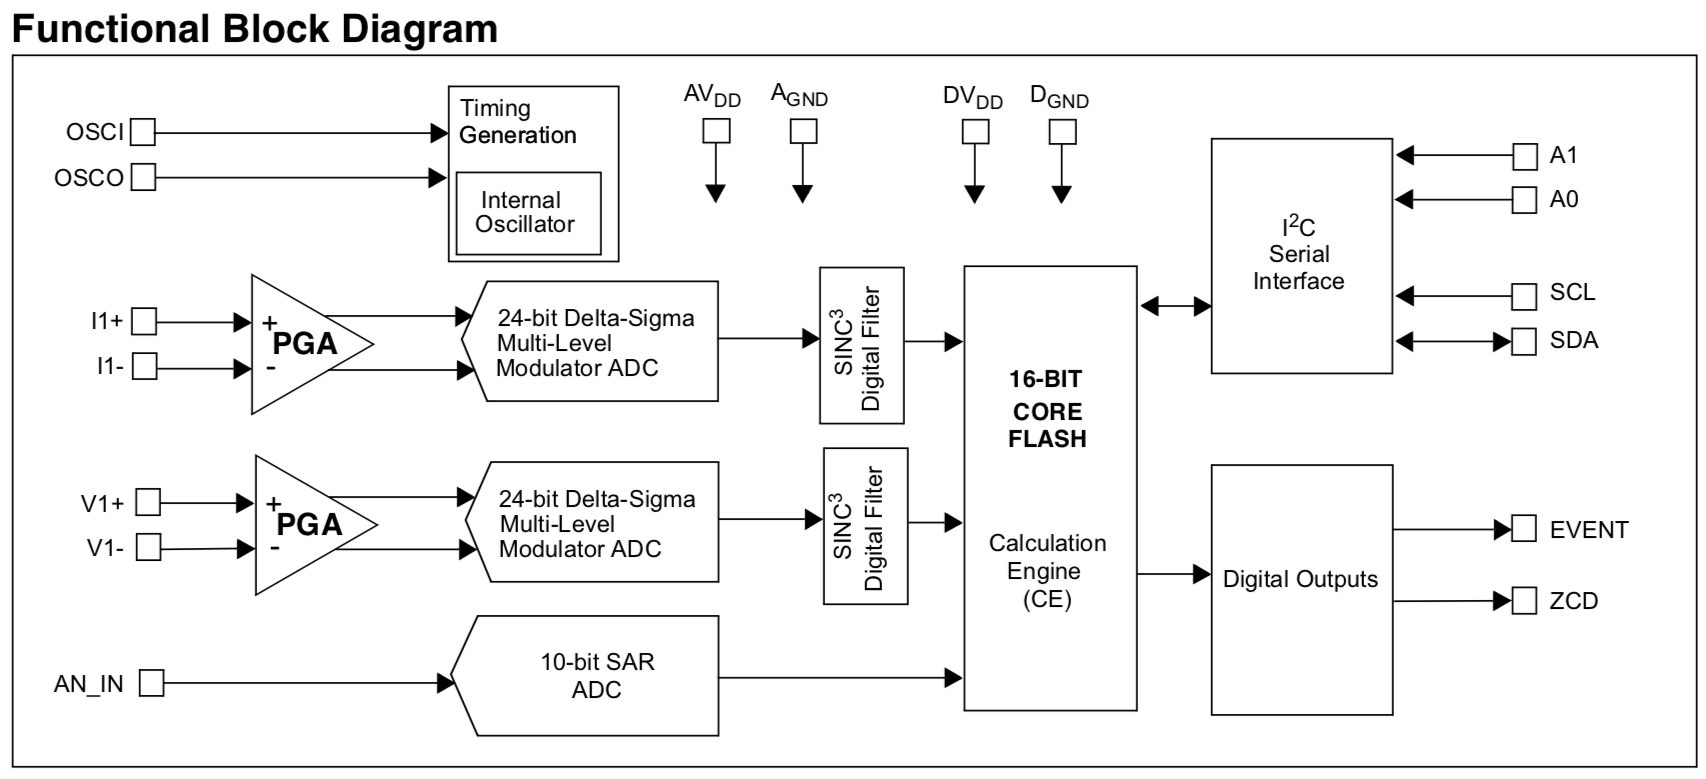
\includegraphics[scale=.4]{Capitulo5/images/MCP_diagrama_funcional.png}
	\caption{Diagrama funcional del dispositivo de adquisición}
	\label{fig:Diagrama funcional}
\end{figure}

\begin{figure}[H]
	\centering
	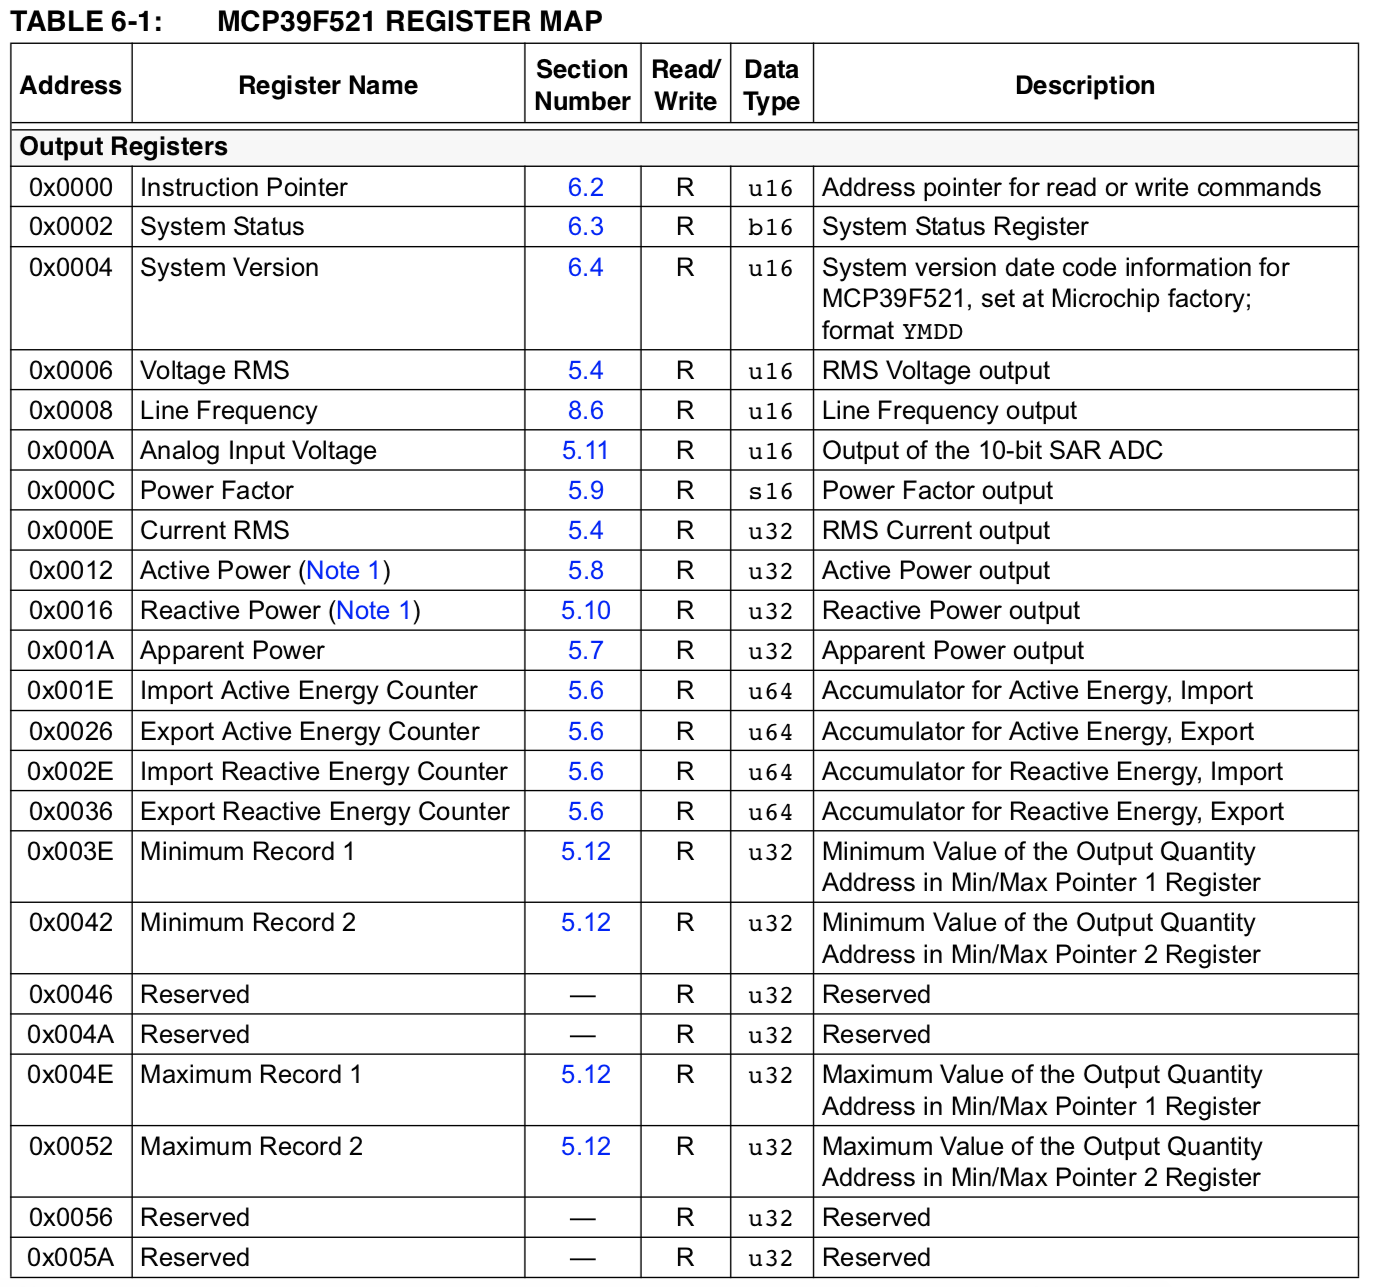
\includegraphics[scale=.5]{Capitulo5/images/register_map.png}
	\caption{Mapa de registros del MCP39F521}
	\label{fig:Mapa de registros del MCP39F521}
\end{figure}

\subsection{Comunicación con el dispositivo de adquisición vía software}

La comunicación IIC con el dispositivo de adquisición a nivel software se realiza, principalmente con los siguientes comandos definidos por el protocolo:

\begin{enumerate}
    \item Inicio de comunicación (START)
    \item Fin de comunicación (STOP)
    \item Acuse de recibo (ACK)
    \item No acuse de recibo (NACK)
    \item Envió de información
    \item Recibo de información
\end{enumerate}

Estas funciones ya están implementadas en lenguaje ensamblador, en una biblioteca denominada I2C.s y nosotros las ocupamos en el programa principal en lenguaje C por medio de su declaración global, en el código siguiente se muestran las rutinas para el comando de inicio de comunicación y envió de datos.

\begin{lstlisting}[language={[x86masm]Assembler}]

;****DECLARACION DE METODOS GLOBALMENTE PARA SU USO EN C*****
.GLOBAL	_START_I2C
.GLOBAL	_ENVIA_DATO_I2C

;************************************************************
ESTA RUTINA GENERA LA CONDICION DE START AL BUS I2C
ENVIANDO CON EL REGISTRO DE CONTROL AL ESCLAVO LA SEÑAL
Y ESPERANDO SU RESPUESTA
;************************************************************
_START_I2C:
	BCLR		IFS0,			#MI2CIF
	BSET		I2CCON,			#SEN
ESPERA_START:
	BTSS		IFS0,			#MI2CIF
	GOTO		ESPERA_START

	RETURN
	
;************************************************************
ESTA RUTINA GENERA LA CONDICION DE ENVIO DE DATO AL BUS I2C
EN ESTE CASO, COPIAMOS LO QUE ESTA EN EL REGISTRO W0 AL 
REGISTRO DE TRANSMISION DE I2C ESPERANDO LA RESPUESTA DEL
ESCLAVO
;************************************************************
_ENVIA_DATO_I2C:
	BCLR		IFS0,			#MI2CIF
	MOV.B		WREG,			I2CTRN
ESPERA_ENVIA_DATO_I2C:
	BTSS		IFS0,			#MI2CIF
	GOTO		ESPERA_ENVIA_DATO_I2C
	
	RETURN
	
\end{lstlisting}

\subsection{Escritura de comandos para el dispositivo de adquisición}

En la figura \ref{fig:Comando de escritura} se muestra la estructura de un byte de control para la escritura de un comando, contiene un bit de inicio, un byte de control que indica hacia qué dispositivo nos dirigiremos, A1 y A0 son los bits de direccionamiento, podemos dirigirnos hacia 4 diferentes dispositivos esclavos, en este caso al tener solo uno, la dirección será “00”, seguido del bit que indica si será una operación de lectura o escritura, al ser escritura toma el valor de cero, formando como byte de control “11101000”.

\begin{figure}[H]
	\centering
	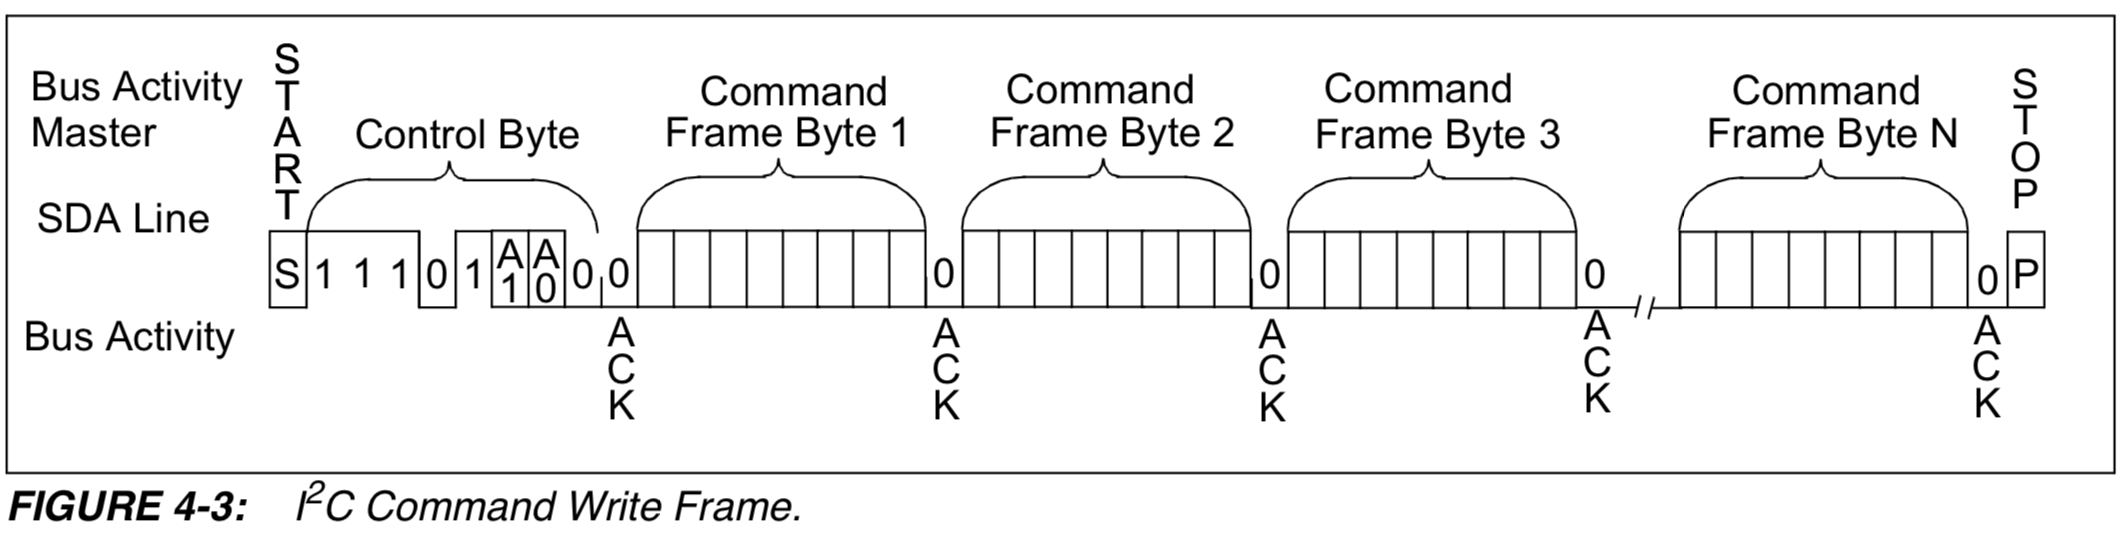
\includegraphics[scale=.4]{Capitulo5/images/write_command.png}
	\caption{Comando de escritura de comando para el dispositivo de adquisición MCP39F521}
	\label{fig:Comando de escritura}
\end{figure}

Este byte de control, indica al dispositivo de adquisición que vamos a iniciar una lectura, este es seguido por un marco o marcos de comandos a ejecutar como se muestra en la figura \ref{fig:Marco de escritura de lectura} , están compuestos por una cabecera, cuantos bytes se recibirán, el o los comandos a ejecutar y un checksum para verificar que la información llego completa y correcta, éste se calcula sumando los datos descritos y dividiéndolos entre 256, el residuo de esta división es el checksum.

\begin{figure}[H]
	\centering
	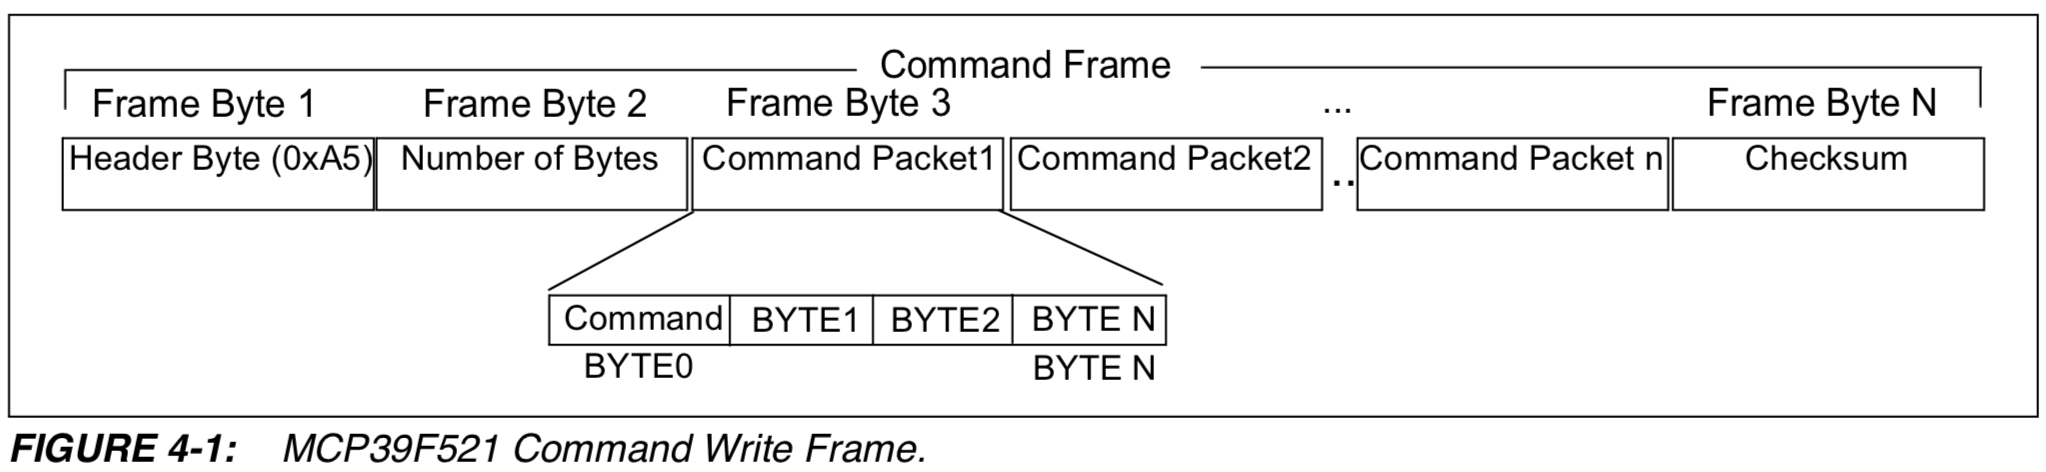
\includegraphics[scale=.4]{Capitulo5/images/marco_write_command.png}
	\caption{Marco para la escritura de un comando de lectura}
	\label{fig:Marco de escritura de lectura}
\end{figure}

Traducido a código en lenguaje c, la rutina que escribe un comando de lectura de registro se ve de la siguiente forma:

\begin{lstlisting}[language={[x86masm]Assembler}]
unsigned char enviaComando ( 
  unsigned char direccion, unsigned char registro, 
  unsigned char bytes, unsigned char checksum )
{
    START_I2C();
 
    //Control byte, write command
    
    ENVIA_DATO_I2C(direccion); //11101000   
    
    if( I2CSTATbits.ACKSTAT == 1 ){ //NACK del sensor
        return NANCK;
    }

    // Inicio del I2C Command Write Frame.
    
    ENVIA_DATO_I2C(0xA5); //header byte
        
    ENVIA_DATO_I2C(0x08); //no. bytes in frame
    
    ENVIA_DATO_I2C(0x41); //command set address pointer
   
    ENVIA_DATO_I2C(0x00); //addr high
     
    ENVIA_DATO_I2C(registro); //addr low 

    ENVIA_DATO_I2C(0x4E); //command read register
    
    ENVIA_DATO_I2C(bytes); //number of bytes to read 
    
    ENVIA_DATO_I2C(checksum); //checksum   
   
    if( I2CSTATbits.ACKSTAT == 1 ){ //NACK del sensor
        return NANCK;
    }
          
    STOP_I2C();
    return EXITO;
}

\end{lstlisting}

Por ejemplo, si queremos conocer el valor de la frecuencia, debemos mandar con la función definida, la señal de inicio de comunicación START y el byte de control de escritura hacia el sensor cero (0xE8), esperar a recibir el acuse de recibo (ACK), enviar la cabecera del marco (A5), el número de bytes que tendrá el marco (contando desde la cabecera hasta el checksum: 0x08), la dirección del registro a leer del mapa, separado en la parte alta y baja (0x00 , 0x08), el comando de lectura de registro (0x4E), el número de bytes a leer, el registro de voltaje tiene una longitud de dos bytes (0x02) y el checksum (0x46), sumado desde el byte de cabecera del marco (0x44) por ultimo, recibiremos el acuse de recibo (ACK) y terminamos la comunicación con un STOP:

\paragraph{}
\framebox[\linewidth]{START() 0xE8 ACK() 0xA5 0x08 0x41 0x00 0x08 0x4E 0x02 0x46 ACK() STOP()}\par

\subsection{Lectura de respuesta del dispositivo de adquisición}

Ahora que logramos comunicarnos con el sensor para requerir la lectura de su o sus registros, necesitamos conocer la respuesta resultante, para ello tenemos que seguir el formato del byte de control de lectura de respuesta del dispositivo esclavo como el fabricante indica y se muestra en la figura \ref{fig:Comando de lectura de respuesta} , tiene un bit de inicio, un byte de control, que nos indica a qué dispositivo esclavo nos dirigimos, en este caso una vez más al “00”, seguido del bit que indica si será una operación de lectura o escritura, al ser lectura toma el valor de uno, formando como byte de control “11101001” seguido de los marcos de respuesta.

\begin{figure}[H]
	\centering
	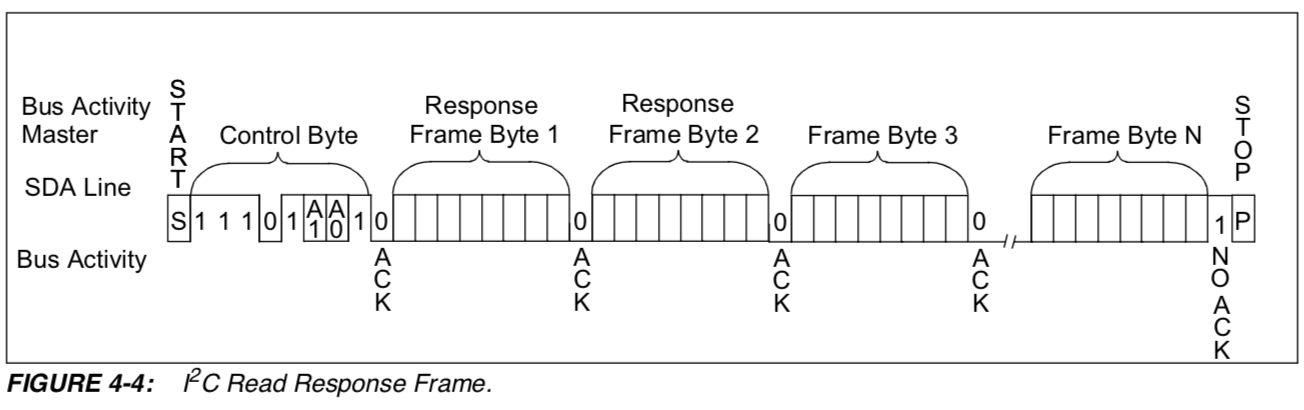
\includegraphics[scale=.7]{Capitulo5/images/read_command.png}
	\caption{Comando de lectura para el dispositivo de adquisición MCP39F521}
	\label{fig:Comando de lectura de respuesta}
\end{figure}

Después del envió del byte de control, recibimos los marcos de respuesta que se muestran en la figura \ref{fig:Marco de respuesta} , que nos indican un acuse especial con valor de 6 hexadecimal, seguido de el numero de bytes que lo conforman, los bytes de información y finalmente un checksum.

\begin{figure}[H]
	\centering
	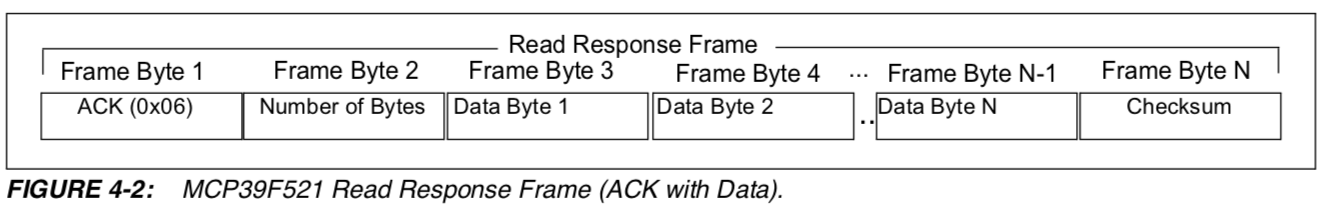
\includegraphics[scale=.7]{Capitulo5/images/responde_frame.png}
	\caption{Marco de respuesta para el dispositivo de adquisición MCP39F521}
	\label{fig:Marco de respuesta}
\end{figure}

Traducido a código en lenguaje c, la rutina que escribe un comando de lectura de respuesta se ve de la siguiente forma:

\begin{lstlisting}[language=C]

unsigned char leeRespuesta(unsigned char direccion)
{   
    
    START_I2C();
    
    //control byte, read response
    
    ENVIA_DATO_I2C(direccion+0x01); //11101001   
    
    if( I2CSTATbits.ACKSTAT == 1 ){ //NACK del sensor
        return NANCK;
    }

    //ack (0x06)
    RECIBE_DATO_I2C();
    ACK_MST_I2C();
    
    //number of bytes 
    int no_bytes = RECIBE_DATO_I2C();
    ACK_MST_I2C();
    
    int i;
    
    //data bytes
    for(i = 0 ; i < no_bytes-3 ; i++){
        U2TXREG = RECIBE_DATO_I2C();
        ACK_MST_I2C();
    }
    
    //checksum
    RECIBE_DATO_I2C();
    NACK_MST_I2C();
    
    STOP_I2C();  
    return EXITO;
}

\end{lstlisting}


Por ejemplo, si queremos leer la respuesta a la lectura del registro de frecuencia, se envía la señal de inicio de comunicación START y el byte de control de lectura hacia el dispositivo cero (0xE9), esperar a leer el acuse de recibo (ACK), el numero de bytes que se reciben del dispositivo esclavo, al valor que se recibe se restan tres bytes: acuse, checksum y numero de bytes (0x05). A continuación de reciben los bytes de datos (0x66 , 0xEA) que finalizan con un checksum y terminamos la comunicación con un STOP:

\paragraph{}
\framebox[\linewidth]{START() 0xE9 ACK() 0x05 0x66 0xEA 0x55 ACK() STOP()}\par

\subsection{Envío de muestras al servidor vía Wi-Fi}

Con estas éstas dos rutinas, conseguimos en bytes, la información de los registros que requiramos con el comando de lectura de registro, para nuestro caso, traeremos el valor del voltaje, corriente, factor de potencia, frecuencia, potencia aparente, activa y reactiva de un panel solar, estos bytes los enviamos por medio del módulo Wi-Fi por medio de la interfaz de comunicación UART, la conexión física de este módulo Wi-Fi es sencilla, usa un estándar de pines para su montura llamado mikrobus (\ref{fig:Mikrobus}), que principalmente tiene un transmisor (TX), receptor (RX), ChipSelect (CS) así como GND y VCC. 

\begin{figure}[H]
	\centering
	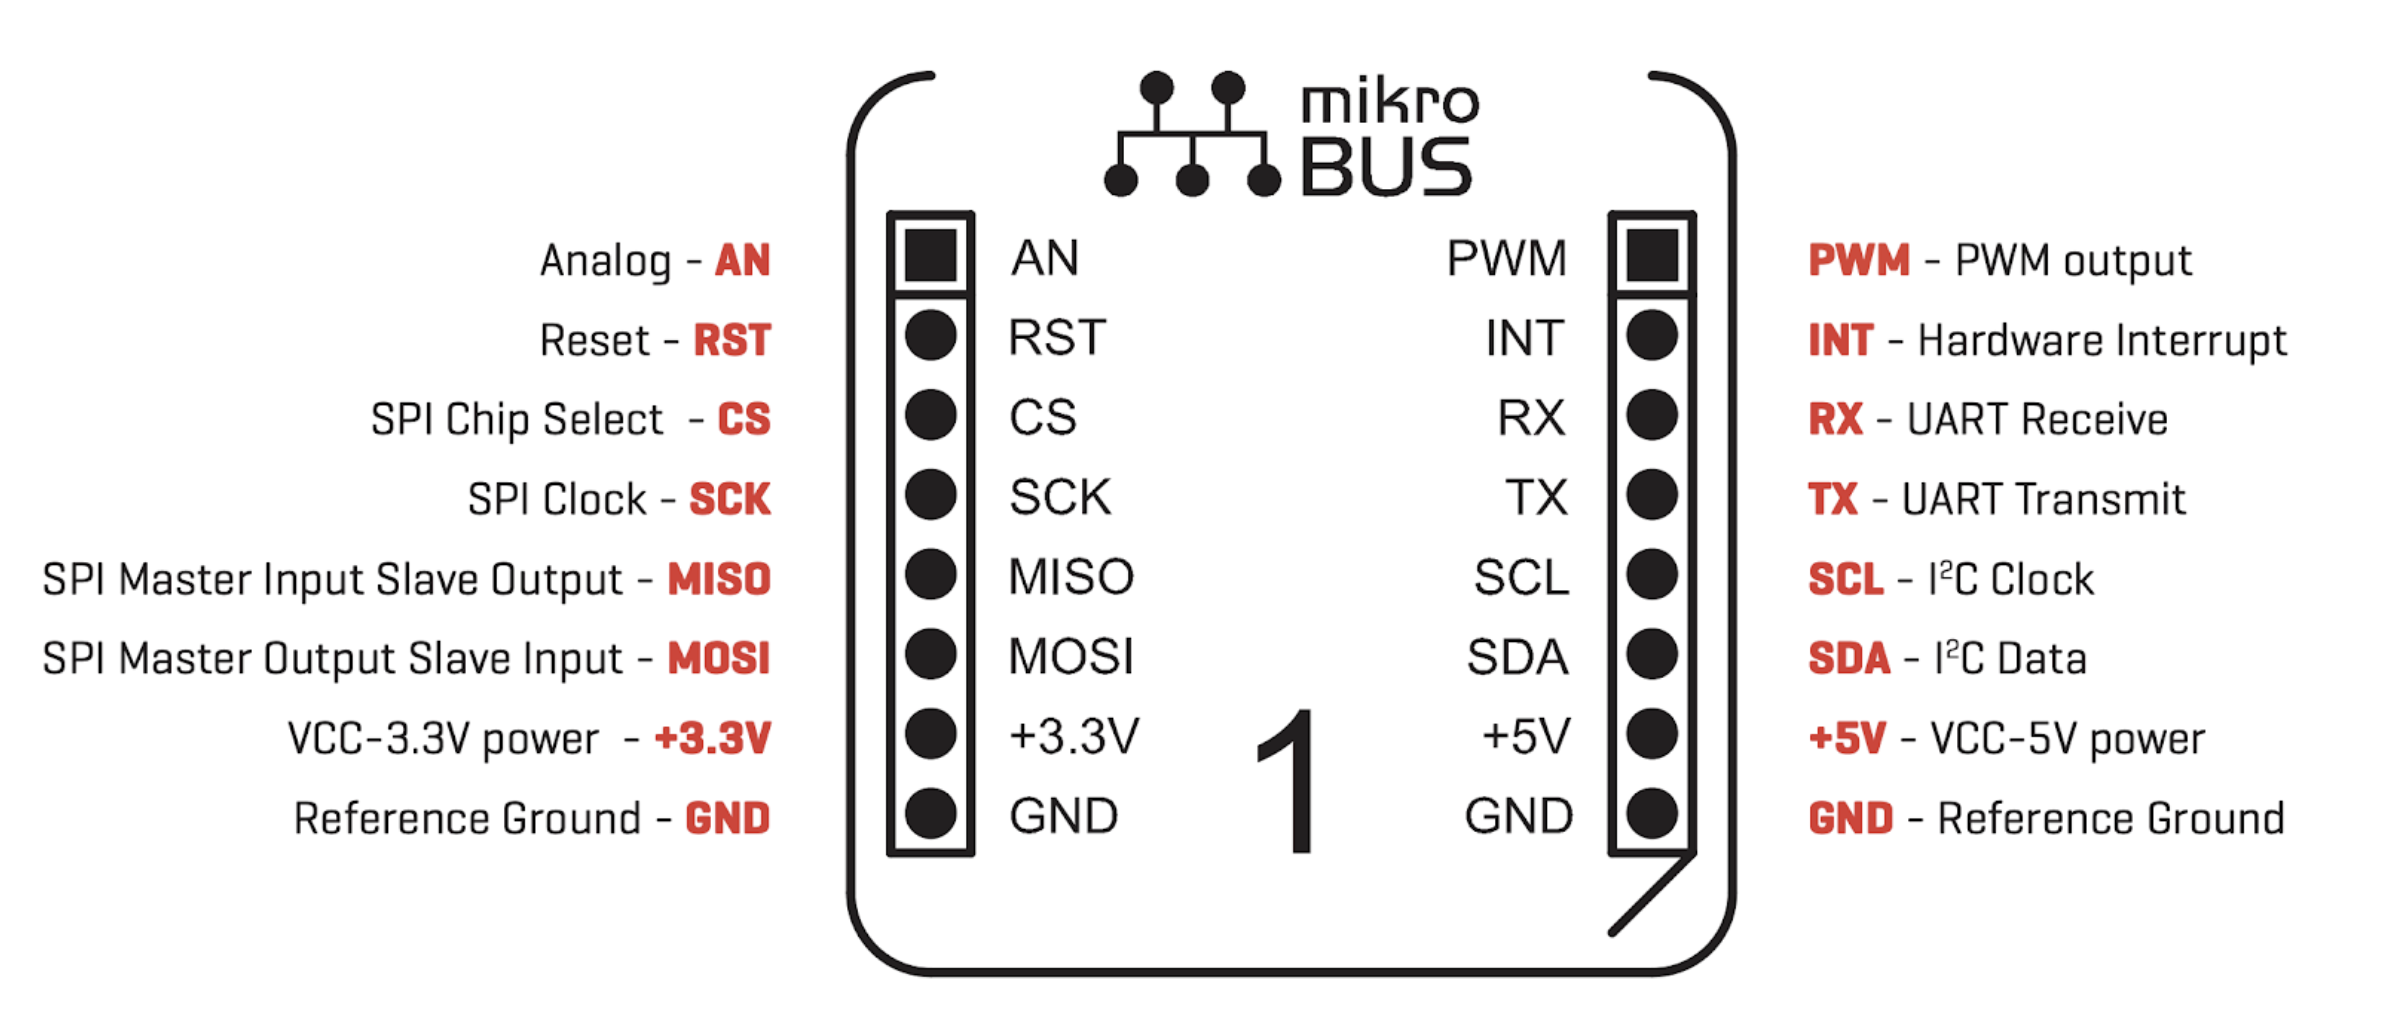
\includegraphics[scale=.2]{Capitulo2/images/mikrobus.png}
	\caption{Estándar de Pines Mikrobus}
	\label{fig:Mikrobus}
\end{figure}

Para poder usar el modulo WiFi a nivel programación, debemos primero, configurar los registros de configuración del modulo UART, el MCP30F4013 tiene 2 interfaces UART, pero la segunda es la que tiene el acomodo para el estándar mikrobus, debemos activar la interfaz UART por medio de su registro de configuración en el microcontrolador, configurar la velocidad de transición de información, esto se calcula dividiendo la frecuencia de trabajo de nuestro microcontrolador (1.8 MHz) entre el Baudaje del módulo Wi-FI, que es de 115200 Baudios.

Después, debemos configurar la interrupción del transmisor UART, de manera que cuando se reciba un dato en el registro receptor, podamos proseguir con otras operaciones sin tener que retardar el proceso de configuración o envío.

\begin{lstlisting}[language=C]

void iniprograma(){
    
    CONTRX = 0;
    
    iniPerifericos();
    
    //UART2 BAUDIOS:115200 mikrobus2 (WIFI)
    U2MODE = 0X0020; //uart disable ,no usa los alternos, autobaudaje
    U2STA  = 0X8000;
    U2BRG  = 0; // (1.8432*10^6)/(16*115200) = 0

    //Interrupciones de uart2 (Modulo wifi))
    IFS1bits.U2RXIF= 0;
    //U2RX interrupts ENABLE
    IEC1bits.U2RXIE= 1;
    
    //Habilitamos el uart2 (Modulo wifi)
    U2MODEbits.UARTEN = 1;
    U2STAbits.UTXEN = 1;
    
    //habilitando el registro de control sensor
    I2CCONbits.I2CEN = 1;
    
    //Inicializamos el modulo wifi
    iniWIFI();
    configWIFI();
}

\end{lstlisting}

Una vez configurada la comunicación UART con el módulo Wi-Fi, es configurar la red del mismo, esto se realiza con comandos AT, dónde configuramos la red a la que nos conectaremos, el protocolo de envió de paquetes, en este caso UDP, a que IP y Puerto nos dirigimos, donde indico la dirección del servidor y cuantos bytes de información se enviarán.

\pagebreak
\begin{lstlisting}[language=C]
//Configuracion del modulo WIFI
void configWIFI(void){  
    
    comandoAT("ATE0\r\n"); //echo off
    sendOK();
    comandoAT("AT+RST\r\n");
    sendOK();
    comandoAT("AT+CWMODE=1\r\n"); //wifi-mode: softAP + station mode
    sendOK();
    comandoAT("AT+CIPMUX=0\r\n"); //disable multiple connections
    sendOK();
    comandoAT("AT+CWJAP=\"CELECSIS\",\"PIC18f2550\"\r\n");
    sendOK();
    comandoAT("AT+CIFSR\r\n"); //get local ip address 
}

//Envio de paquetes
void enviaWIFI(void){
    
    comandoAT("AT+CIPSTART=\"UDP\",\"104.198.212.166\",4000\r\n");
    sendOK();
    comandoAT("AT+CIPSEND=21\r\n");
    sendOK();
    
    //---Colocar aquí los nodos existentes---//
    
    //---Enviando numero de serie de microcontolador (AA)
    numero de sensor (0) y su informacion ---//
    U2TXREG = 'A';
    U2TXREG = 'A';

    U2TXREG = 0x00;

    leeTransmiteSensor(0xE8);
    sendOK();
    //----------------------------------------//   
    
    
    comandoAT("AT+CIPCLOSE\r\n");
    sendOK();
    
}
\end{lstlisting}

En la función principal, se envían muestras al servidor, no exactamente cada segundo, hicimos pruebas y cubre 50 muestras al minuto y hacemos un reinicio cada 30 minutos por si hay algún tipo de falla con la conexión de red.

\begin{lstlisting}[language=C]
//programa principal
int main (void)
{     
    iniprograma();

    //reinicio del programa cada media hora
    int counter = 0;
    
    //enviamos muestras cada segundo y reiniciamos el sistema cada media hora
    for(;EVER;)
    {           
        enviaWIFI();
        
        counter = counter+1;
        
        if(counter == 900){
            iniprograma();
            counter = 0;
        }
        
        __delay_ms(500);
    }
    
    return 0;
}
\end{lstlisting}

Si queremos verlo en un plano mas general o como lógica pura, nos podemos apoyar en el diagrama de flujo \ref{fig:logica micro} que sintetiza el trabajo del microcontrolador.

\begin{figure}[H]
	\centering
	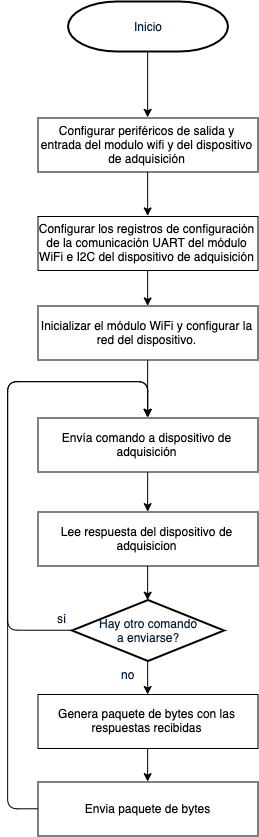
\includegraphics[scale=.5]{Capitulo5/images/logica_micro.png}
	\caption{Lógica programada en el microcontrolador}
	\label{fig:logica micro}
\end{figure} 

Físicamente, la figura \ref{fig:conexion hardware} muestra como se hace la conexión entre microcontrolador con dispositivo de adquisición, el montaje del modulo Wi-Fi, la conexión del panel solar a la carga y su inyección a la linea eléctrica.
    
\begin{figure}[H]
	\centering
	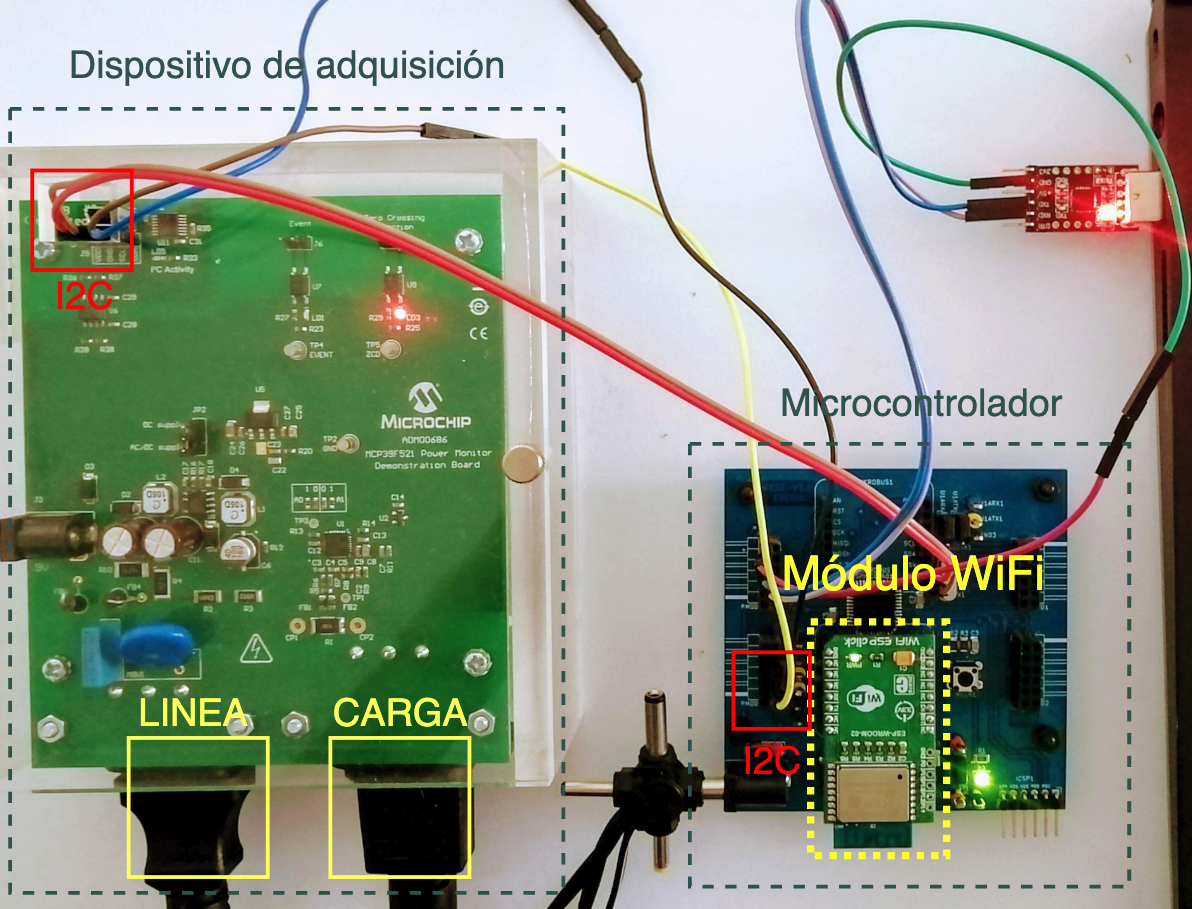
\includegraphics[scale=.3]{Capitulo5/images/conexion_fisica.png}
	\caption{Conexión de hardware del sistema}
	\label{fig:conexion hardware}
\end{figure} 

\subsubsection{Pruebas}
\textbf{Tipo :} Unitaria de Funcionalidad \\ \newline

Para probar el funcionamiento de la comunicación con el dispositivo de adquisición via IIC, se conecto un cable USB con comunicación UART al microcontrolador, que copia los mismos datos que se envían al modulo Wi-Fi, a una computadora, solamente agregamos los pines del UART1 en la configuración del programa y copiamos en su registro de transmisión los datos conseguidos, nos basamos en el ejemplo de la hoja técnica para comparar el resultado conseguido.

\begin{figure}[H]
	\centering
	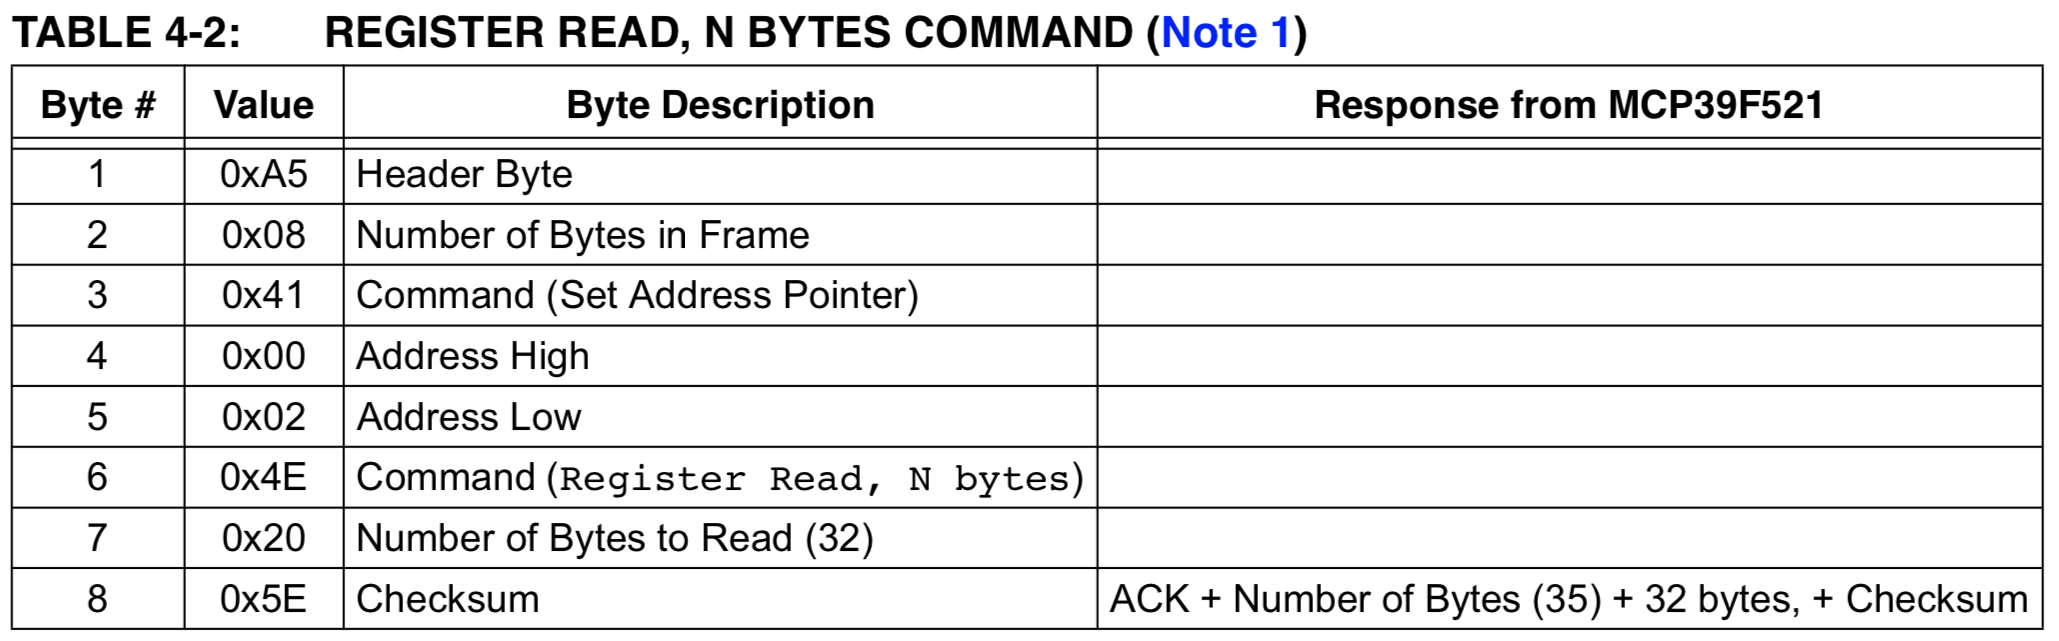
\includegraphics[scale=.3]{Capitulo5/images/respuesta_sensor.png}
	\caption{Respuesta del sensor a un comando de lectura determinado}
	\label{fig:respuesta sensor}
\end{figure} 

En la consola de la computadora, vemos la siguiente información impresa en pantalla,  podemos interpretarla de la siguiente forma:

\begin{itemize}
    \item Los dos primeros valores 255 nos marcan el fin de la transmisión
    \item ACK de la respuesta del esclavo (6 en ascii).
    \item Número de bytes (35)
    \item Los siguientes 32 datos son los datos enviados por el dispositivo esclavo del estado del sistema según el mapa de registros \ref{fig:Mapa de registros del MCP39F521} .
    \item El 170 es el checksum del envío de la trama, podemos comprobarlo sumando desde el valor del acuse (6) hasta el penúltimo dato, dando un total de 1706 decimal, si dividimos esto entre 256, el valor del checksum será igual al residuo de la división, que es igual a 170.
\end{itemize}

\begin{figure}[H]
	\centering
	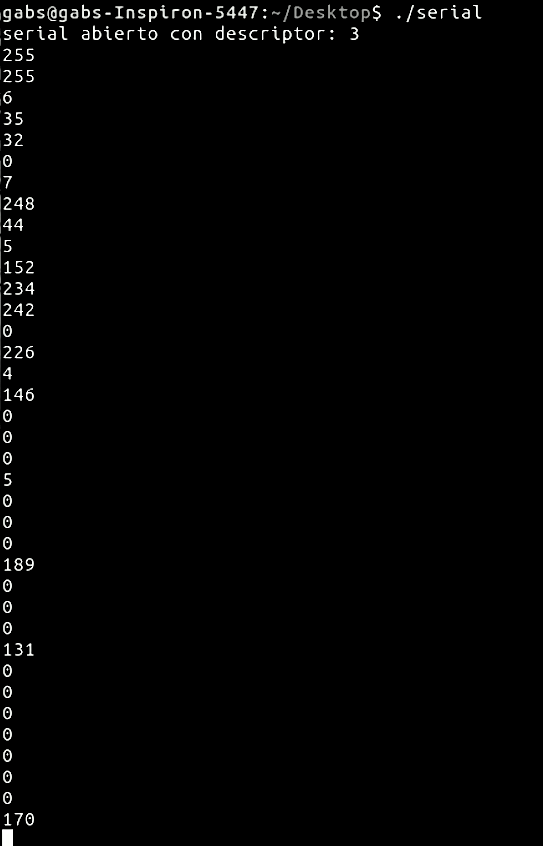
\includegraphics[scale=.3]{Capitulo5/images/consola.png}
	\caption{Respuesta proveniente del sensor a un comando de lectura de su registro}
	\label{fig:consola}
\end{figure} 

\subsubsection{Pruebas}
\textbf{Tipo :} Integración \\ \newline

La ultima funcionalidad por probar es el envió de muestras al servidor, lo único que tenemos que hacer, es crear un servidor UDP en la IP y Puerto indicados en el programa del microcontrolador para la captura de los paquetes:


\begin{lstlisting}[language=Python]
import socket
import sys
import datetime, time
import os
import struct

#---------------Variables de configuracion-----------------
server_ip = '10.128.0.2'
port = 4000
#----------------------------------------------------------

# Creando socket UDP
sock = socket.socket(socket.SOCK_DGRAM, socket.SOCK_DGRAM)

# Relacionar direccion IP con puerto
server_address = (server_ip, port)
sock.bind(server_address)

print ('Starting up server on %s port %s' % server_address)

# Esperando por conexion
while True:

    print('Waiting for a connection...')
    
    pack, client_connection = sock.recvfrom(21)

    #Recibiendo paquete de 21 bytes
    pack = struct.unpack('21B',pack)

    packet = pack

    #Imprimir paquete recibido
    print(packet)

\end{lstlisting}

Y el resultado de este programa, es la captura de paquetes que tienen una longitud de 21 Bytes:
\begin{itemize}
    \item Byte 1 y 2: El numero de serie del microcontrolador en código ASCII.
    \item Byte 3: El numero de esclavo.
    \item Byte 4 y 5 : El valor del voltaje.
    \item Byte 6 y 7 : El valor de la frecuencia.
    \item Byte 8 y 9 : El valor de la corriente.
    \item Byte 10,11,12 y 13 : El valor de la potencia aparente.
    \item Byte 14,15,16 y 17 : El valor de la potencia activa.
    \item Byte 18,19,20 y 21 : El valor del factor de potencia.
\end{itemize}

Los valores que tienen mas de un byte, son enviados empezando por el byte menos significativo y terminando con el byte más significativo, esto es porque son valores decimales, a los bytes que se consiguen se les hace un corrimiento de bits para conseguir el valor original.
A continuación se muestra la captura de paquetes UDP procedentes del microcontrolador, cada paquete trae 21 bytes que se muestran en valor decimal en consola:

\begin{figure}[H]
	\centering
	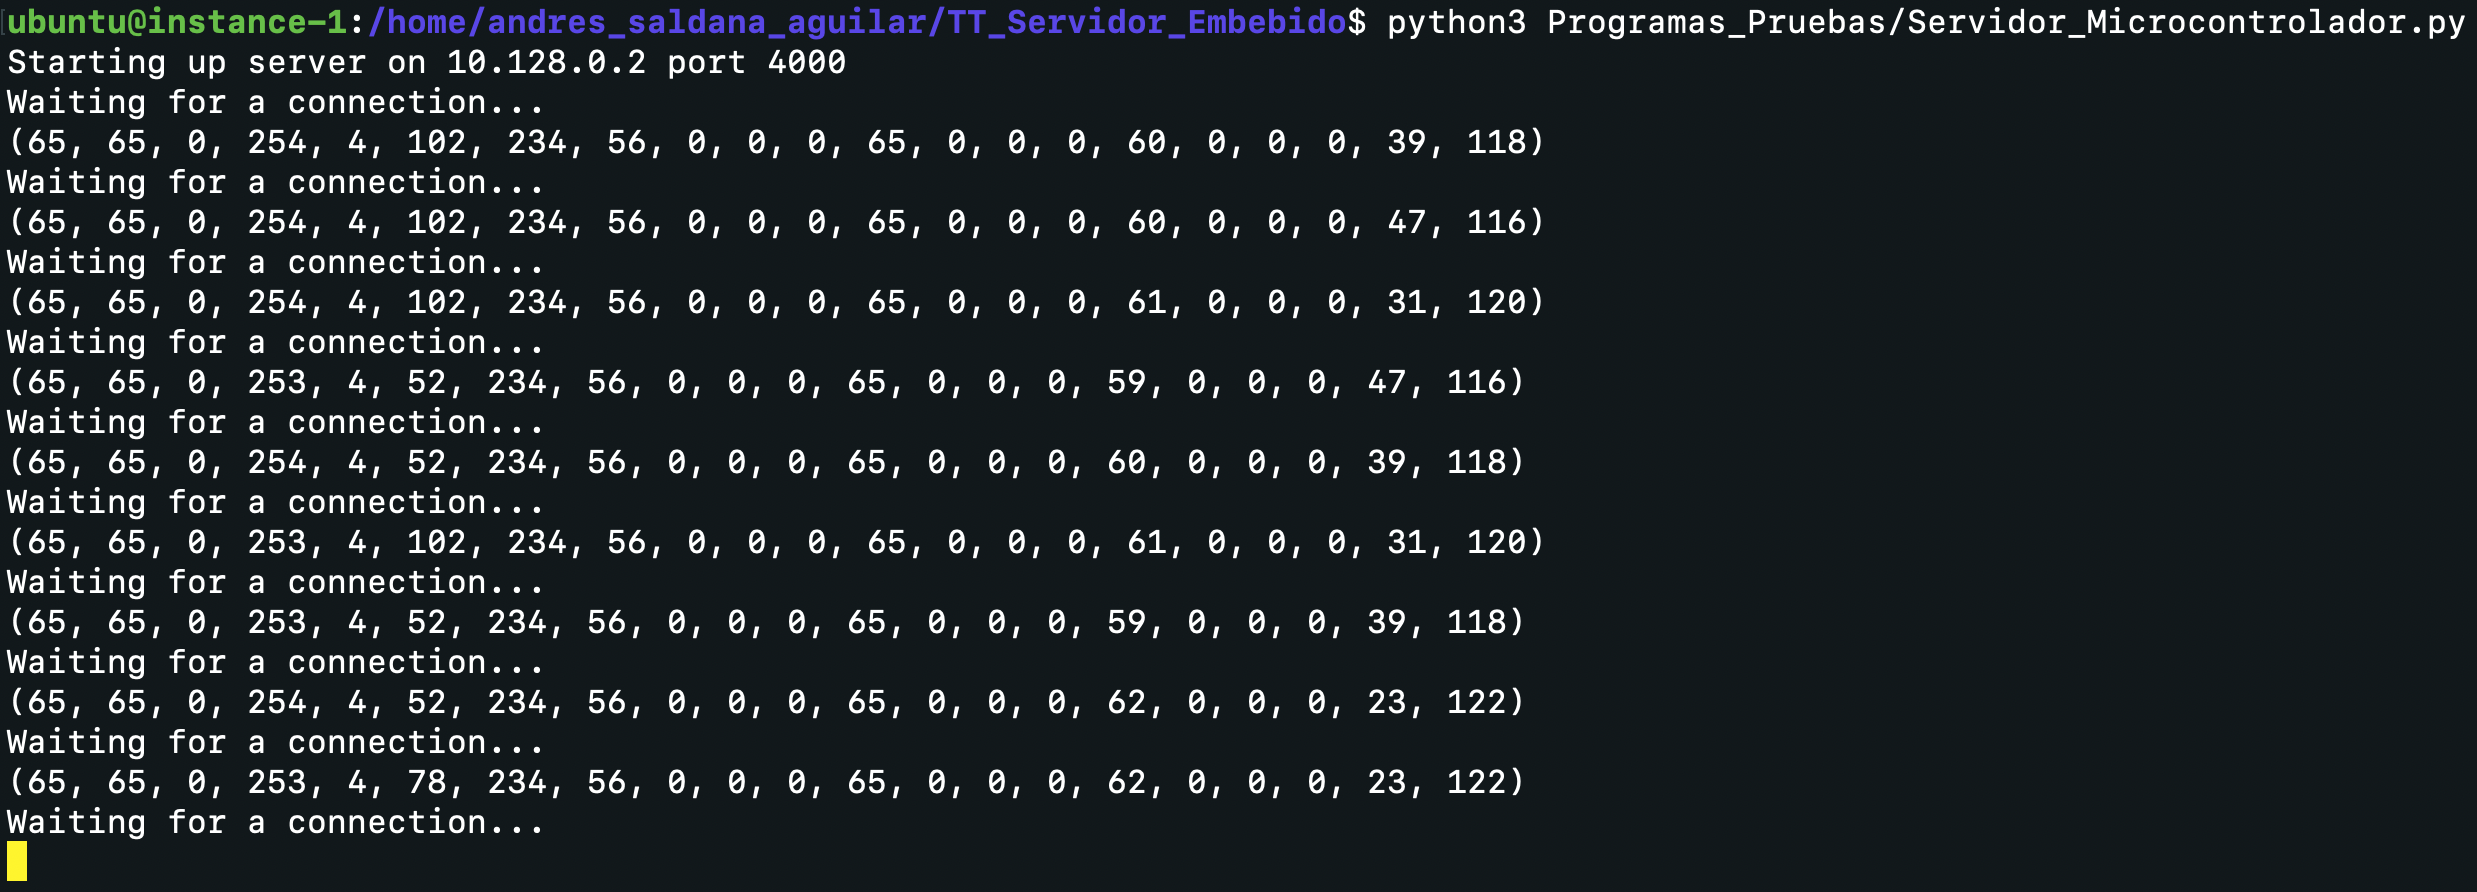
\includegraphics[scale=.3]{Capitulo5/images/paquetes_recibidos.png}
	\caption{Programa capturador de paquetes enviados por el microcontrolador en valor decimal}
	\label{fig:respuesta sensor}
\end{figure} 


De está manera se concluye la funcionalidad de la obtención y envió vía Wi-Fi de mediciones de potencia producida por un panel solar.

\section{Módulo del Servidor Embebido}

\subsection{Objetivo}
Implementar la funcionalidad descrita en los casos de uso \ref{SUB-M-CU1.3} (SUB-M-CU1.3), \ref{SUB-M-CU1.4} (SUB-M-CU1.4) y \ref{SUB-M-CU1.5} (SUB-M-CU1.5), dónde indicamos que nuestros servicios estarán alojados en un servidor web en el sistema embebido RaspBerry Pi 3. Los servicios que este ofrecerá son:

\begin{itemize}
    \item Configurar el entorno del servidor embebido
    \item Capturar y consumir paquetes UDP provenientes de los distintos microcontroladores para el calculo de producción de energía, monitoreo y gráficas \ref{SUB-M-CU1.3} (SUB-M-CU1.3).
    \item Consultar y almacenar cada minuto la generación de cada nodo \ref{SUB-M-CU1.5} (SUB-M-CU1.5).
    \item Atender a las peticiones de la aplicación móvil sobre la información de un nodo o de la red de sensores \ref{SUB-M-CU1.4} (SUB-M-CU1.4).
\end{itemize}

\subsection{Configurar el servidor embebido}

\subsubsection{Desarrollo}

Utilizaremos el SBC Raspberry Pi 3 \citep{MarcoTeorico19} como servidor de aplicaciones y almacén de datos, para poder lograr esto, usaremos como sistema operativo Ubuntu Core de Linux, especialmente hecha para esta tarjeta, los pasos para cargar la imagen del sistema se describen en \citep{InstallUbuntuCore}, los pasos son:

\begin{itemize}
    \item Descargar la imagen de Ubuntu Core (2.42 GB) de la página oficial de Canonical.
    \item Formatear una memoria MicroSD (en nuestro caso con una capacidad de 16GB) y copiar en el la imagen de Ubuntu Core en él.
    \item Introducir la memoria en la ranura de la Raspberry Pi 3, conectar a el un cable Ethernet un teclado y monitor.
\end{itemize}

Para formatear la memoria, utilizamos la herramienta de MacOS de gestión de discos, que nos permite formatear volúmenes en el formato DOS FAT 32 que requiere la imagen, debemos asignarle un nombre al volumen que deberemos recordar para el siguiente paso, el resultado del formato se muestra en la figura \ref{fig:formato}.
 
\begin{figure}[H]
	\centering
	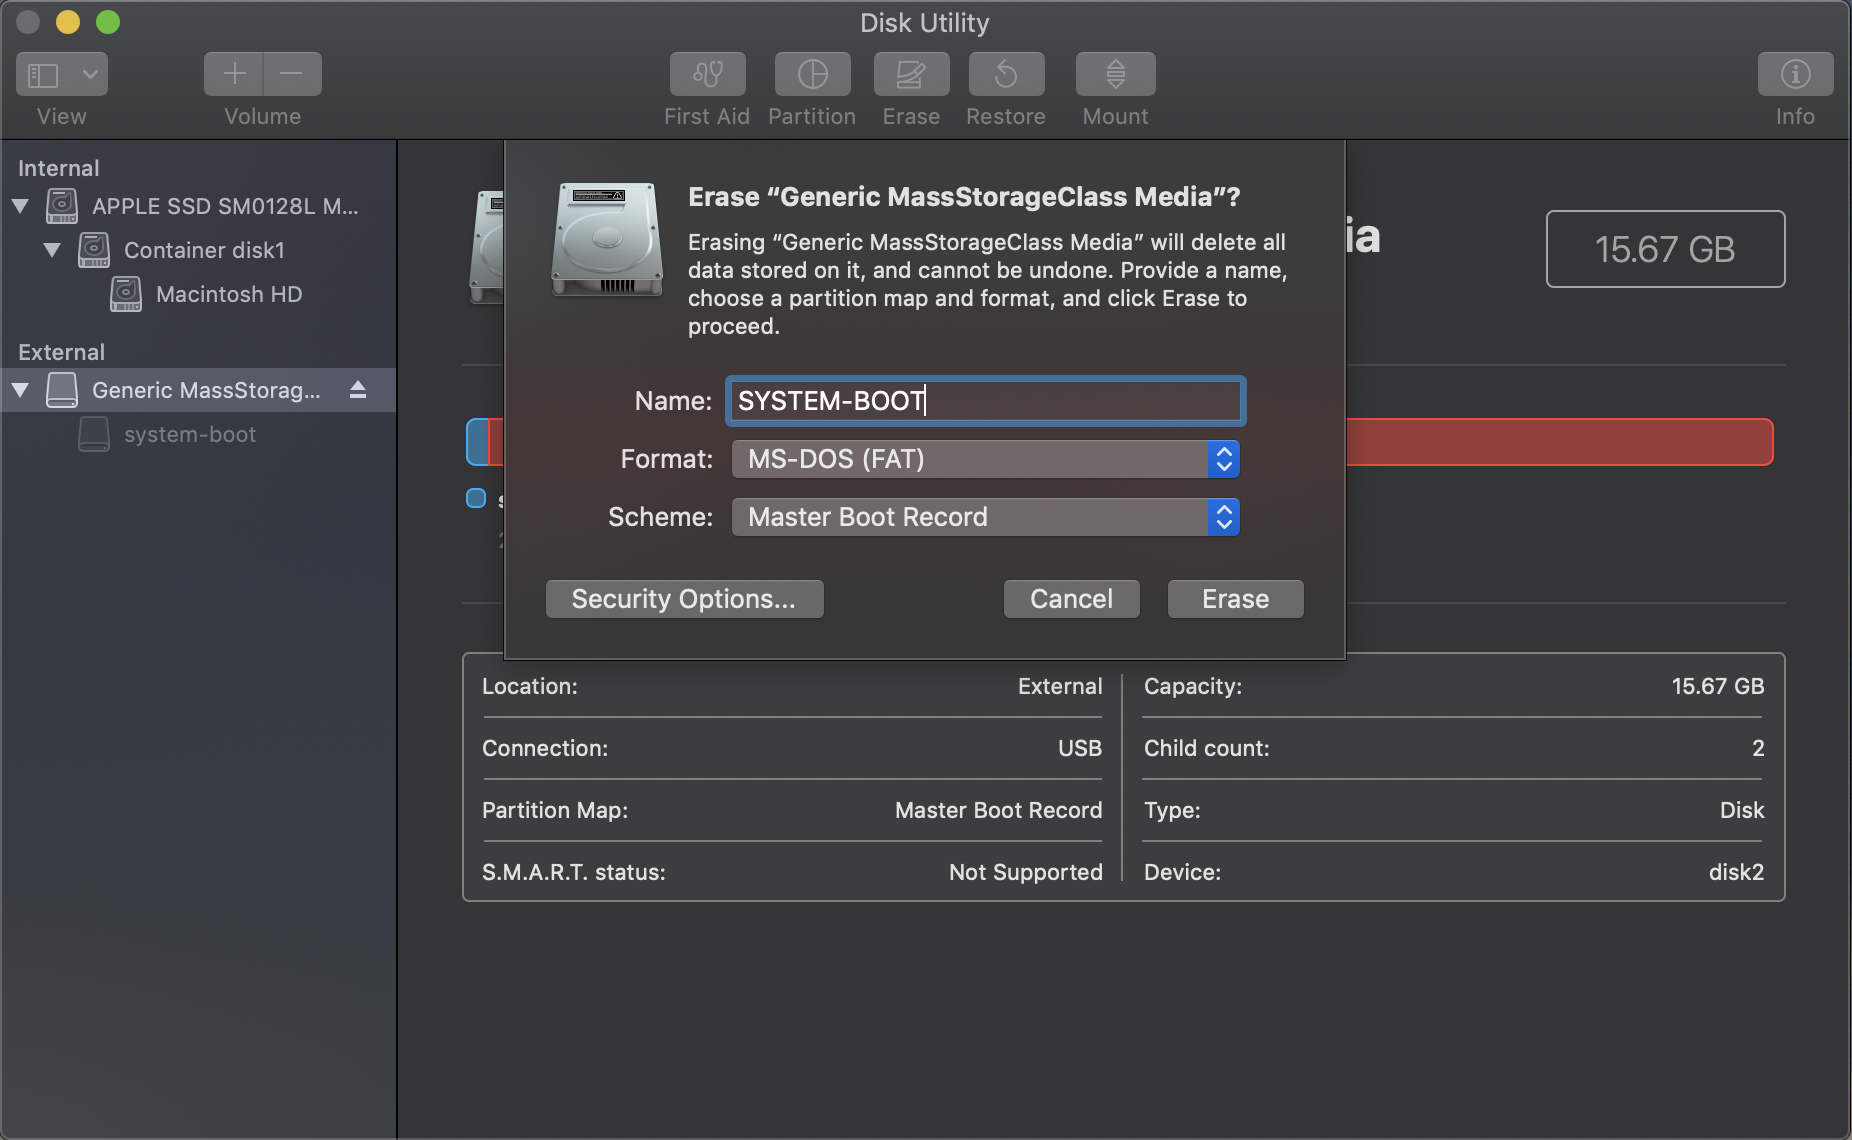
\includegraphics[scale=.3]{Capitulo5/images/format.png}
	\caption{Dando formato a la tarjeta SD}
	\label{fig:formato}
\end{figure} 

Ahora debemos desmontar el volumen y copiar en el la imagen descargada, para conocer el nombre del volumen de la memoria usamos el comando \hl{diskutil list}, buscando la ruta con el nombre de nuestro volumen y lo desmontamos con el comando \hl{diskutil unmountDisk rutaVolumen} el resultado de estos dos comandos se muestra en la figura \ref{fig:desmonataje}.

\begin{figure}[H]
	\centering
	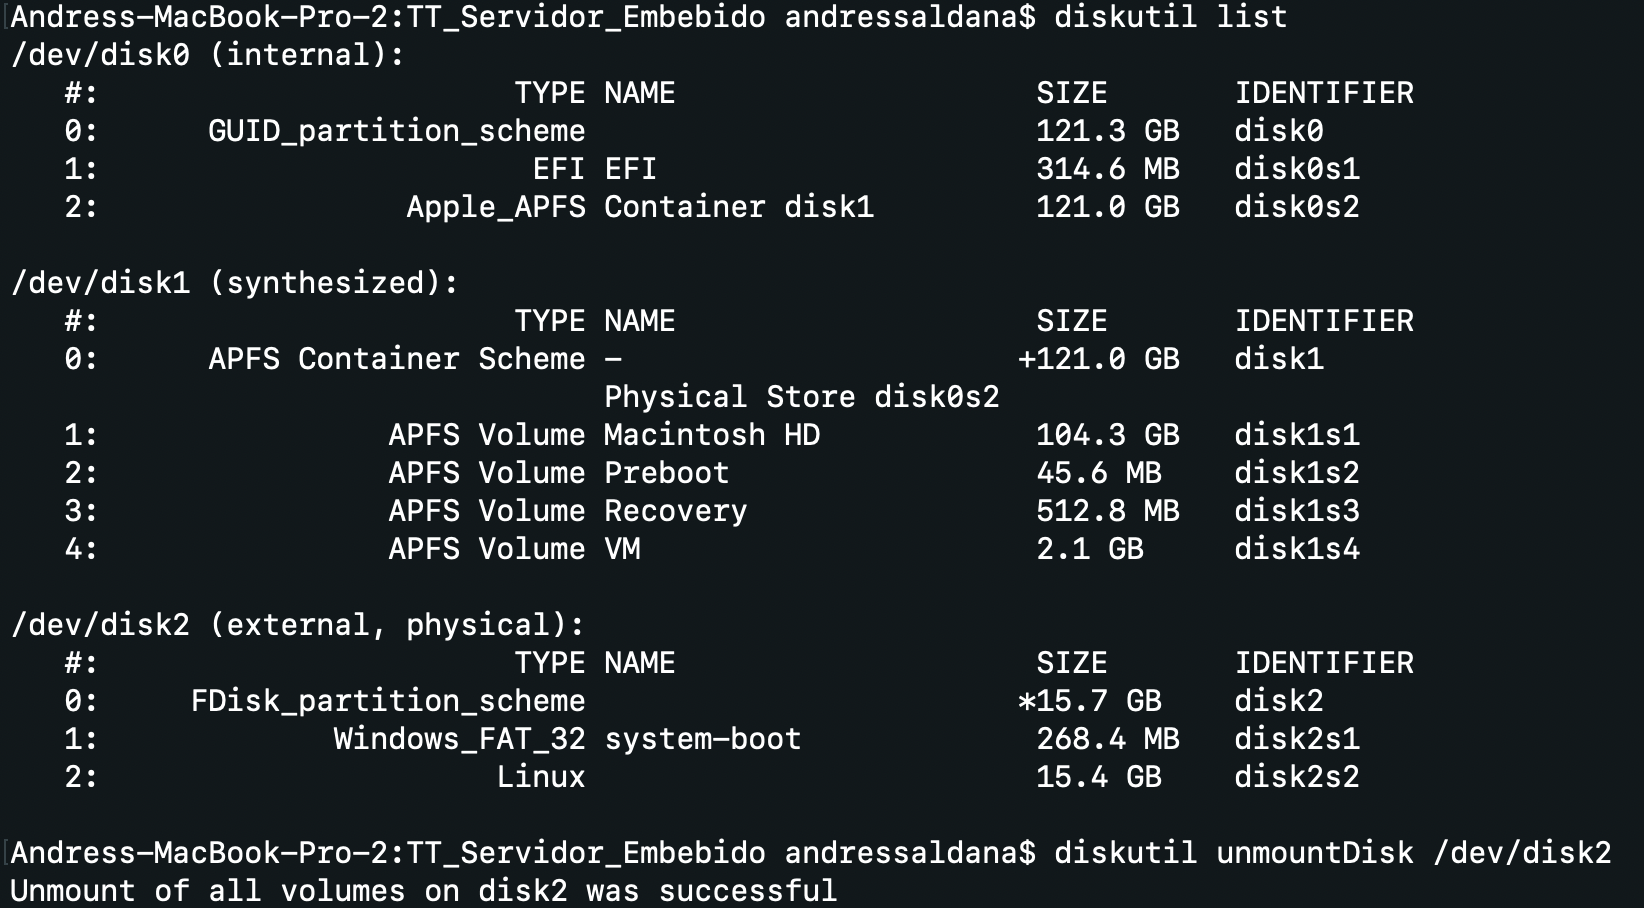
\includegraphics[scale=.4]{Capitulo5/images/unmount.png}
	\caption{Desmontando volumen de memoria SD}
	\label{fig:desmonataje}
\end{figure} 

Copiamos la imagen del sistema operativo a la memoria con el comando \hl{lsudo sh -c 'gunzip -c ~/rutaImagen.img.xz   | sudo dd of=rutaVolumen bs=32m} y nos debe dar una salida en consola como la que se muestra en la figura \ref{fig:copia}.

\begin{figure}[H]
	\centering
	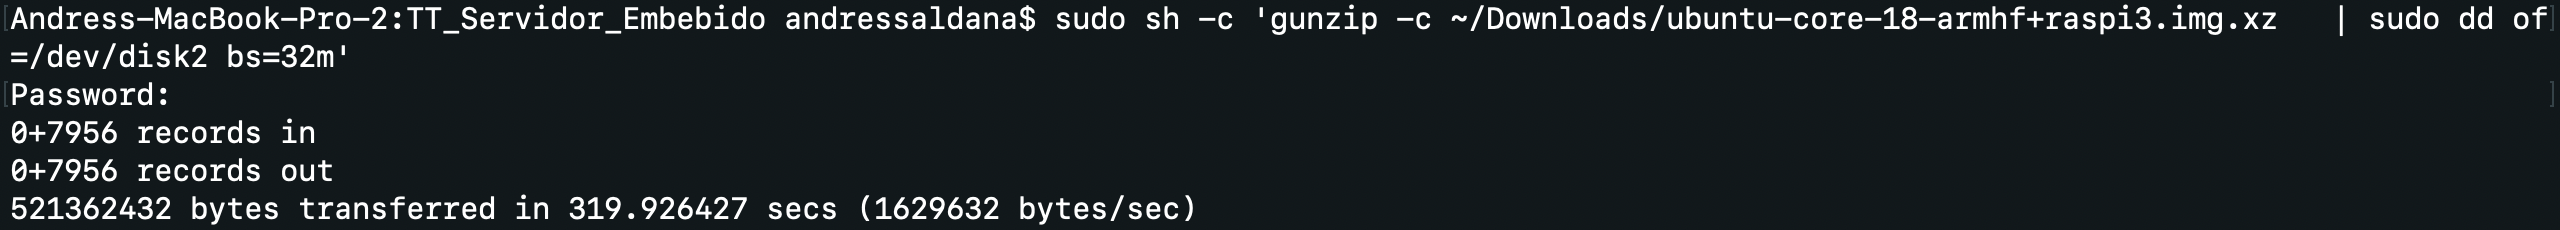
\includegraphics[scale=.3]{Capitulo5/images/copyimg.png}
	\caption{Copiando imagen de sistema operativo a memoria SD}
	\label{fig:copia}
\end{figure} 

\subsubsection{Pruebas}
\textbf{Tipo :} Unitaria de Funcionalidad \\ \newline

Ahora conectamos la Raspberry un monitor con un cable HDMI, un cable ethernet hacia el módem telefónico, un teclado y a la fuente de alimentación como se muestra en la figura \ref{fig:conexion}, debemos crear una cuenta en Ubuntu para asociar un correo electrónico a una llave pública para poder hacer el inicio de sesión remotamente vía ssh, la llave publica se genera con el comando \hl{ssh-keygen -t rsa -b 4096 -C correoasociado@gmail.com} que nos generará dos llaves como se muestra en la figura \ref{fig:llave}, debemos copiar el contenido de la llave pública a el llavero de Ubuntu en su página como se muestra en la figura \ref{fig:ubuntullave}, finalmente, el sistema embebido nos mostrará un mensaje como el de la figura \ref{fig:primer arranque} con el que nos indicara como iniciar sesión vía SSH, ingresando ese comando en una computadora podemos acceder al sistema embebido remotamente \ref{fig:login} 

\begin{figure}[H]
	\centering
	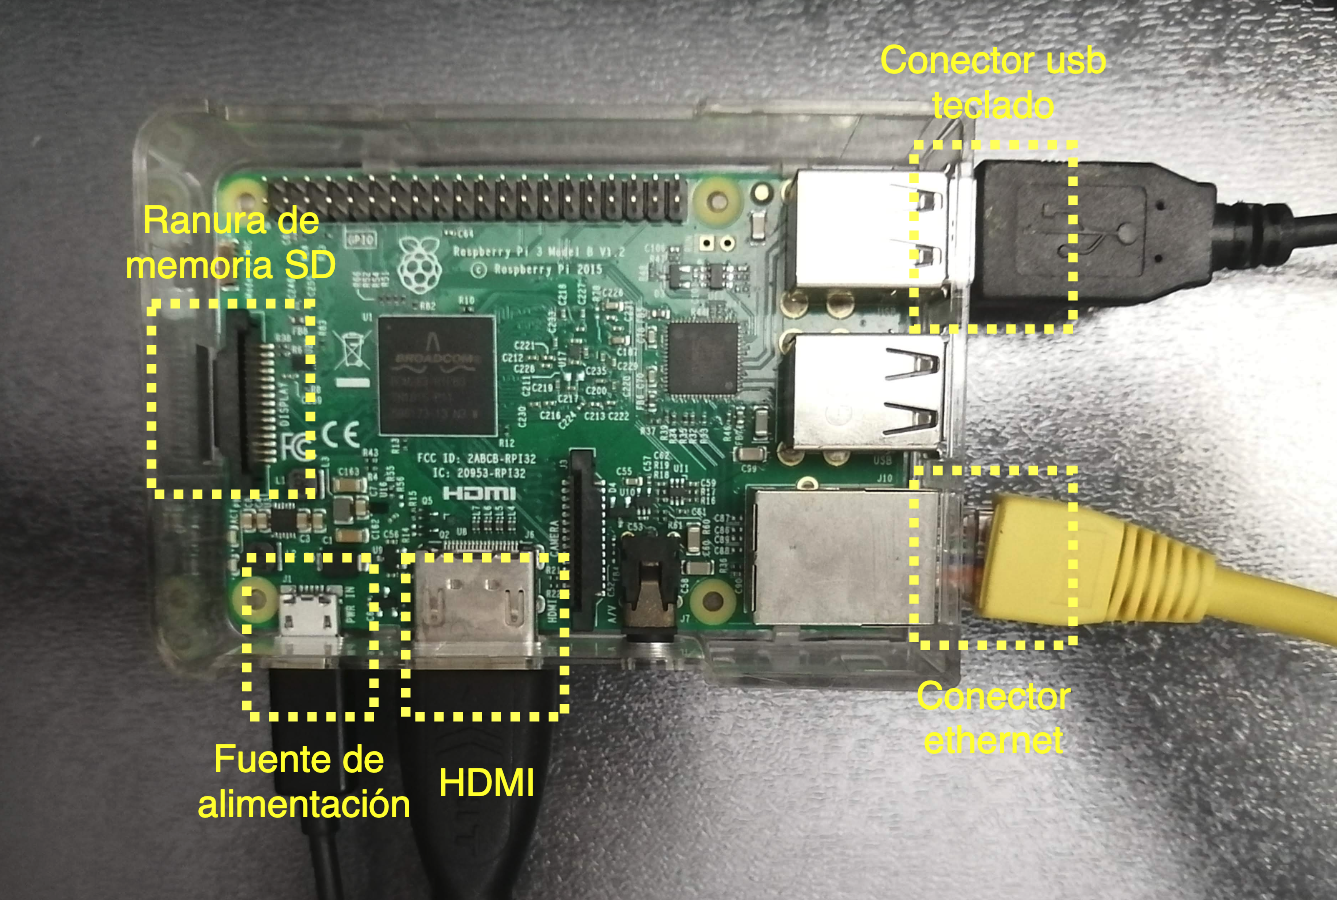
\includegraphics[scale=.25]{Capitulo5/images/rasp.png}
	\caption{Conexión de Raspberry}
	\label{fig:conexion}
\end{figure} 

\begin{figure}[H]
	\centering
	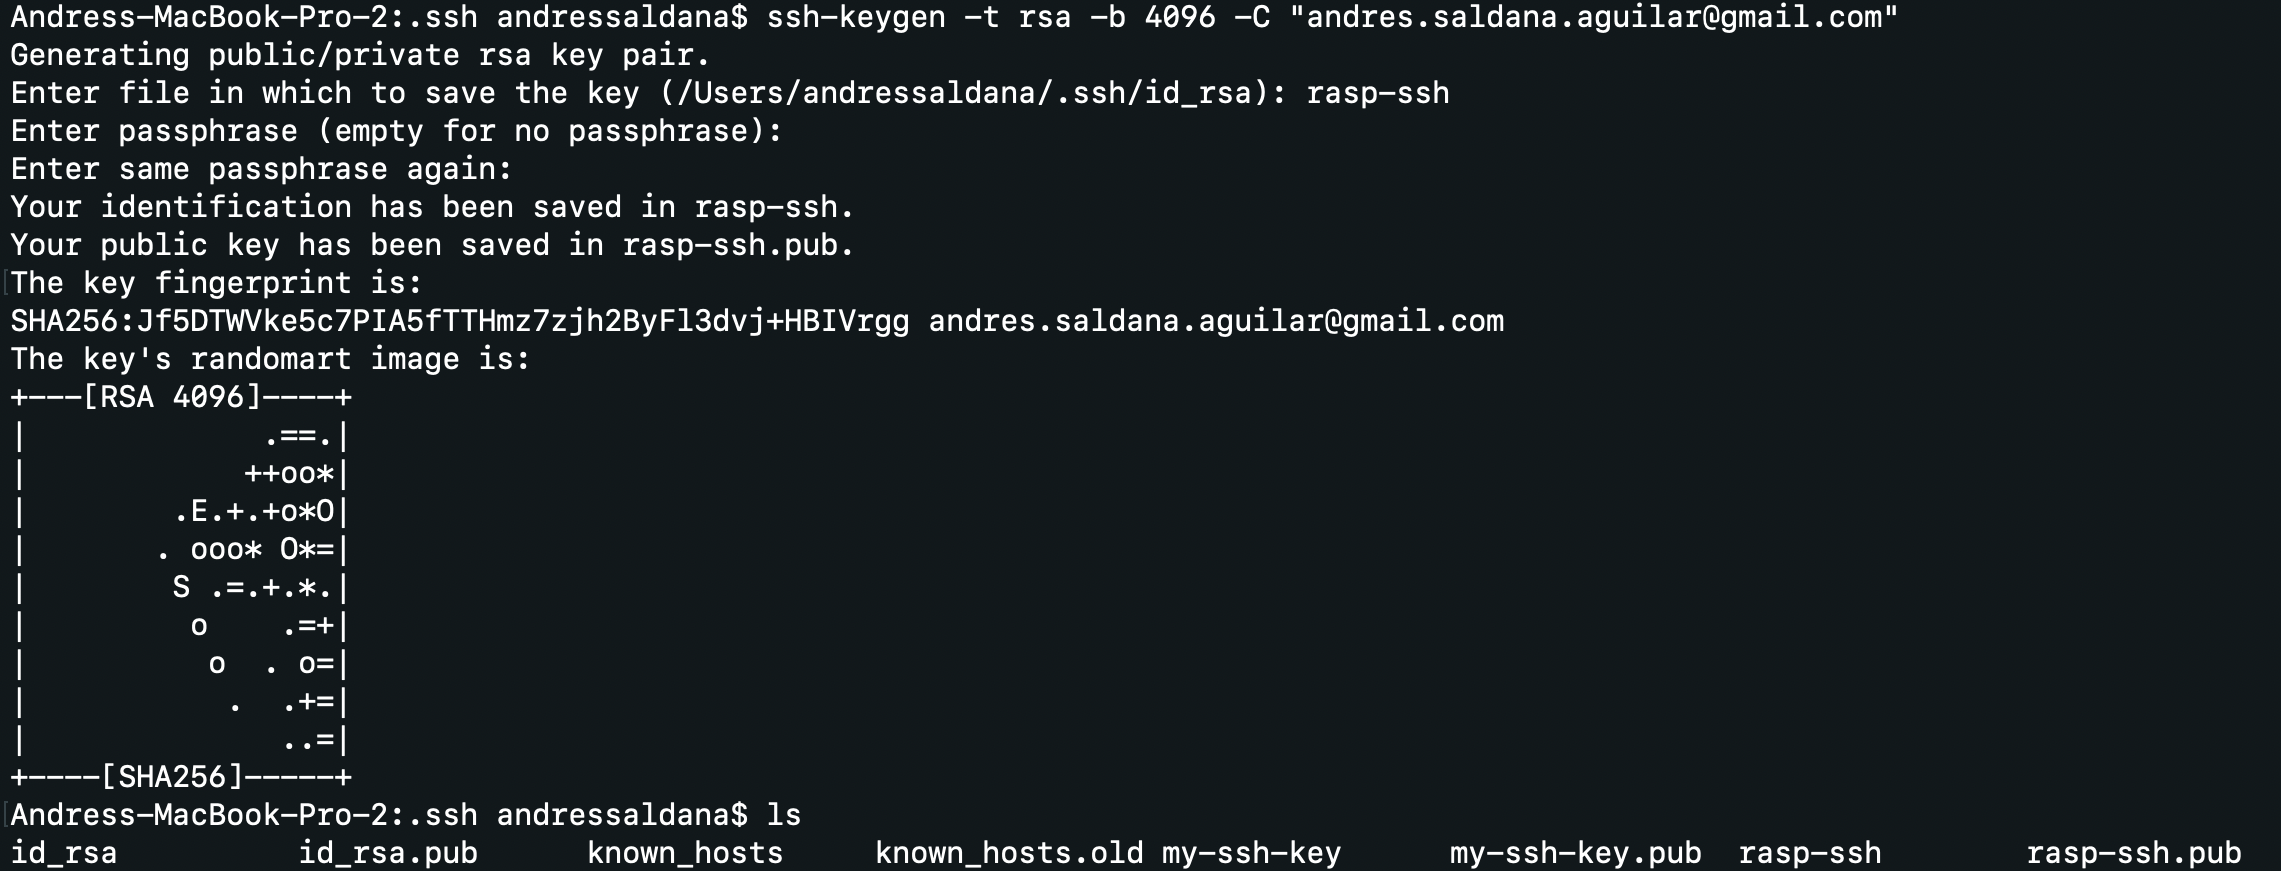
\includegraphics[scale=.3]{Capitulo5/images/ssh_keygen.png}
	\caption{Generando llave pública}
	\label{fig:llave}
\end{figure} 

\begin{figure}[H]
	\centering
	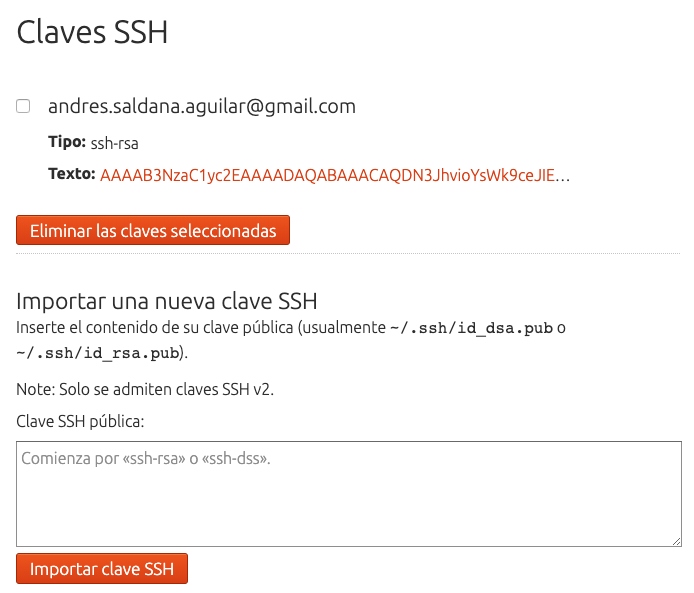
\includegraphics[scale=.3]{Capitulo5/images/sshkey.png}
	\caption{Agregando la llave pública a la cuenta asociada a Ubuntu}
	\label{fig:ubuntullave}
\end{figure} 

\begin{figure}[H]
	\centering
	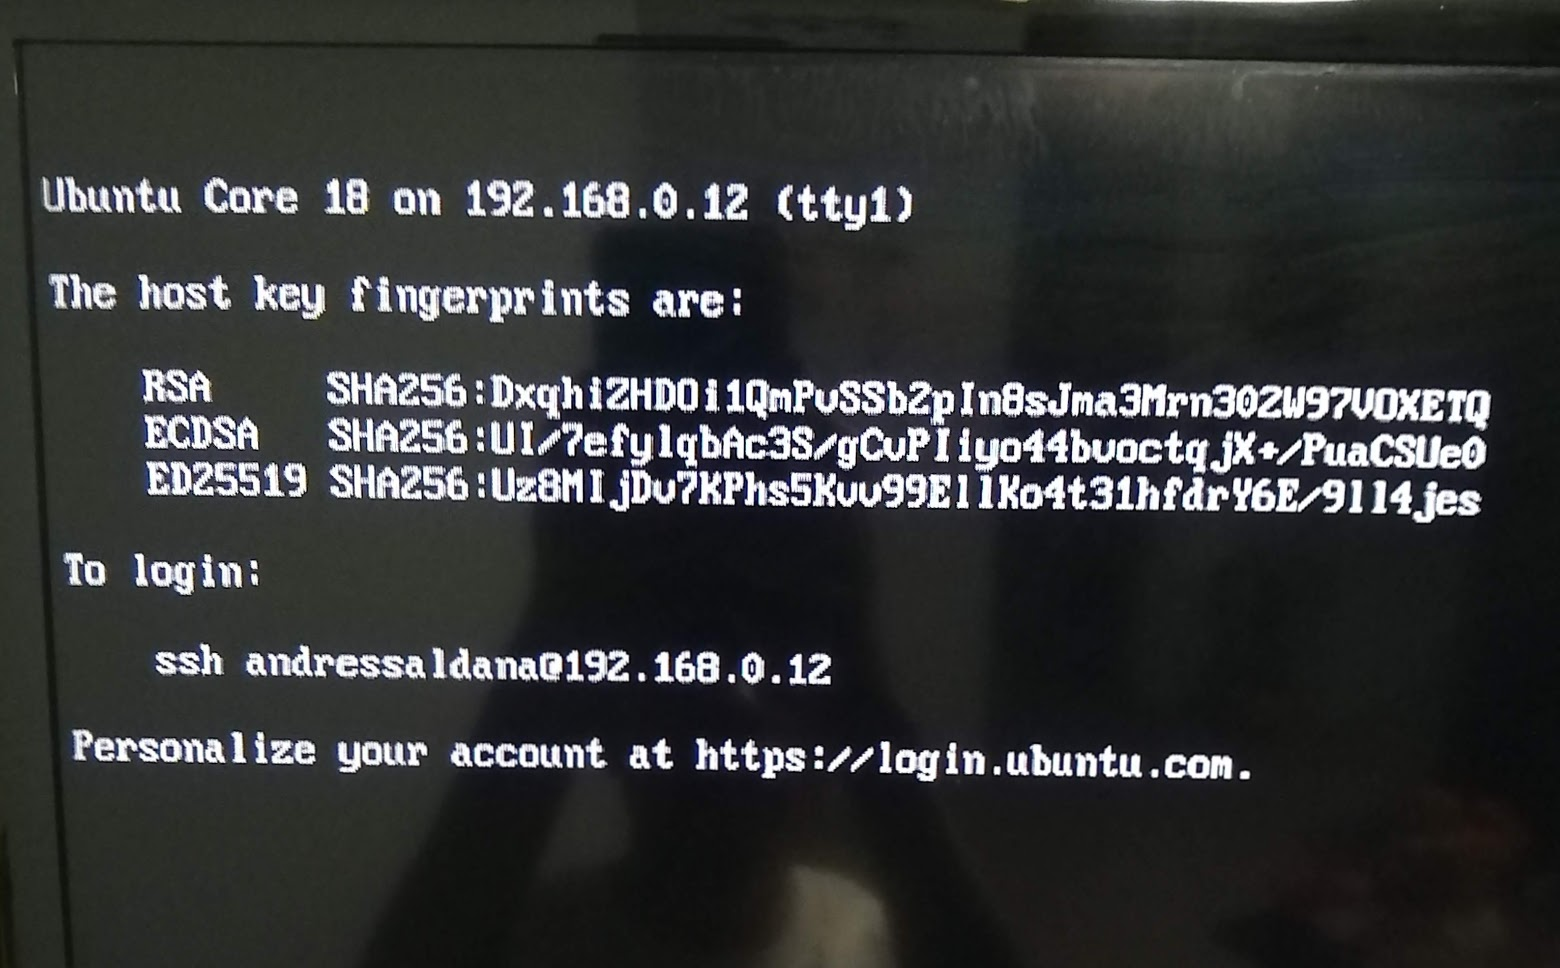
\includegraphics[scale=.15]{Capitulo5/images/first_boot.jpg}
	\caption{Primer arranque del sistema listo para ser utilizado}
	\label{fig:primer arranque}
\end{figure} 

\begin{figure}[H]
	\centering
	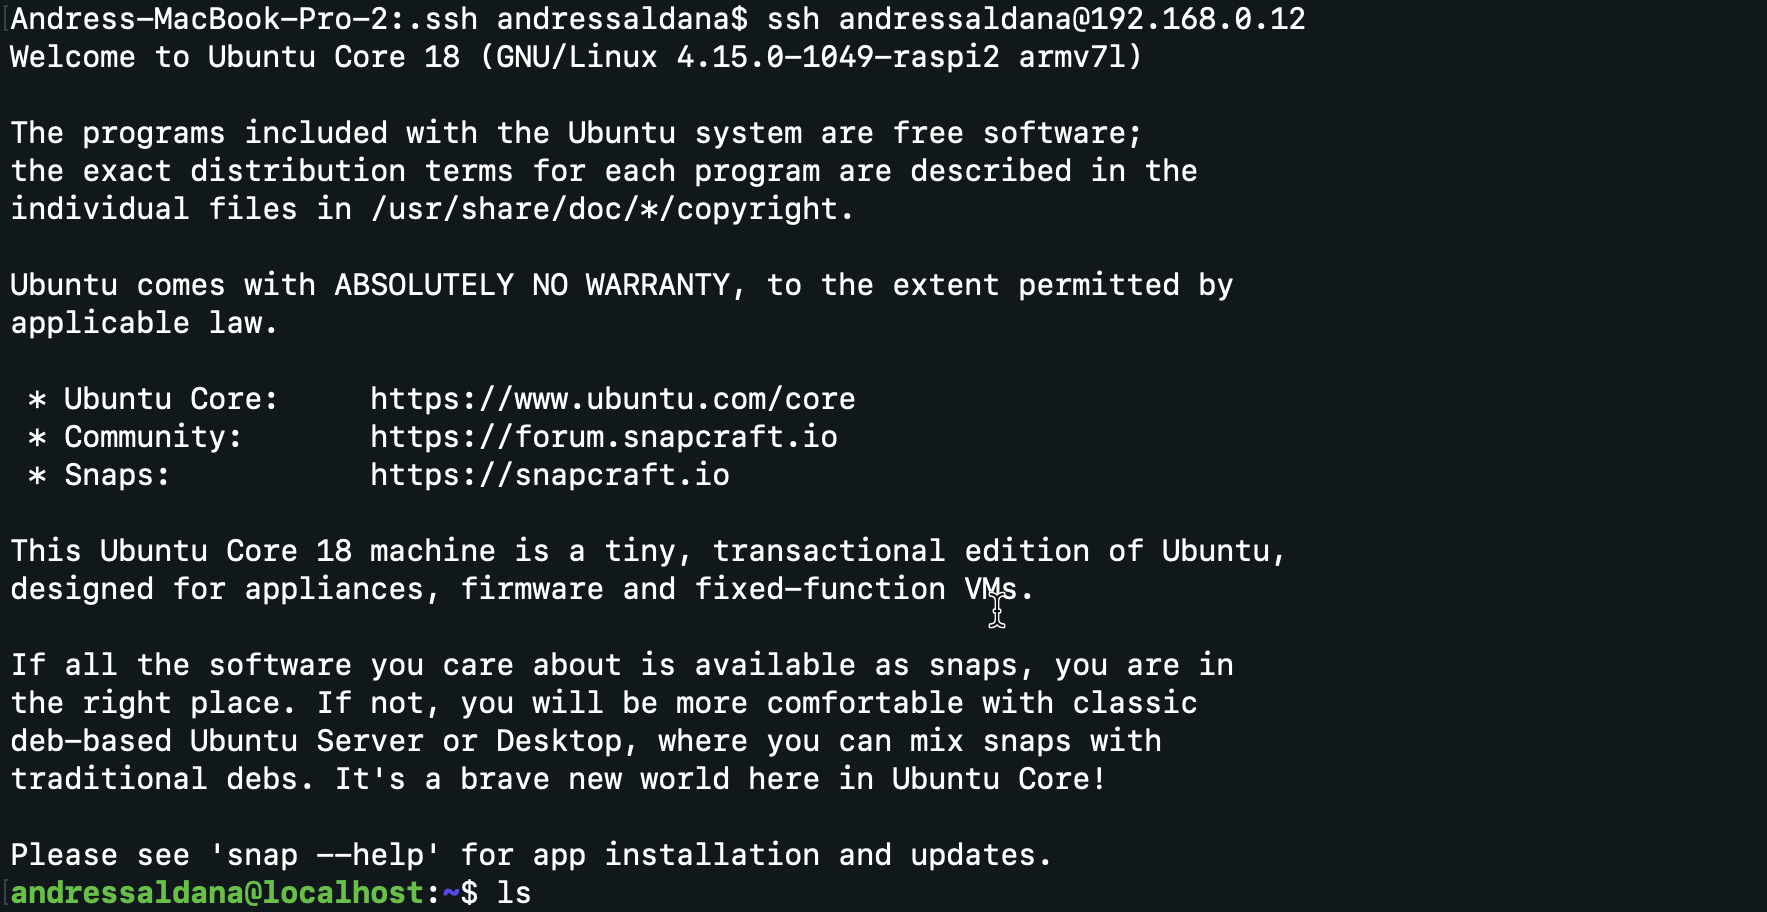
\includegraphics[scale=.3]{Capitulo5/images/login.png}
	\caption{Acceso al servidor embebido de manera remota via SSH}
	\label{fig:login}
\end{figure} 


Con estos pasos, ya tenemos un servidor que es capaz de correr aplicaciones, almacenar hasta 13GB de información en nuestro caso por la capacidad de la memoria SD y con conexión a la red local o inclusive pública si contamos con un proveedor de internet que nos proporcione una IP pública.


\subsection{Creando servicios en Ubuntu Linux}

Todos los programas a implementar serán ejecutados en el sistema embebido como servicios, para ello debemos crear un archivo de configuración por cada uno de los servicios que se ofrecerán con el comando \hl{sudo vi /lib/systemd/system/nombreServicio.service} en el que escribiremos la siguiente configuración:

\begin{lstlisting}
[Unit]
Description=Dummy Service
After=multi-user.target
Conflicts=getty@tty1.service

[Service]
Type=simple
ExecStart=/usr/bin/python3 /direccion/de/programa.py
StandardInput=tty-force

[Install]
WantedBy=multi-user.target
\end{lstlisting}

Reiniciamos el contenedor de demonios del sistema con \hl{sudo systemctl daemon-reload} , habilitamos el servicio que creamos con \hl{sudo systemctl enable nombreServicio.service} e iniciamos su ejecución con \hl{sudo systemctl start nombreServicio.service}, por ultimo podemos usar el comando \hl{sudo systemctl status nombreServicio.service} para conocer el estado del servicio como se muestra en la figura \ref{fig:systemctl}.

\begin{figure}[H]
	\centering
	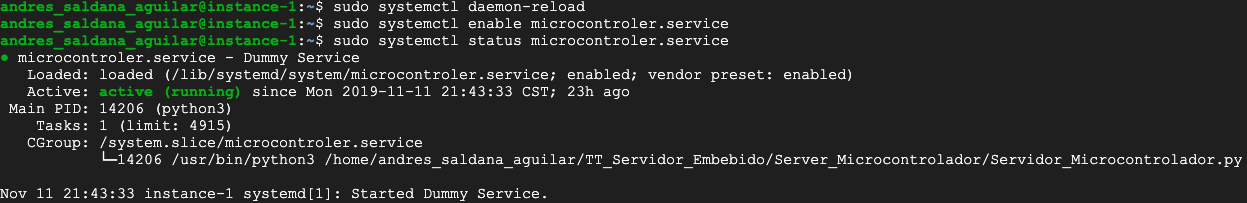
\includegraphics[scale=.35]{Capitulo5/images/systemctl_tests.png}
	\caption{Resultado de los comandos de manejo de servicios en Linux Ubuntu}
	\label{fig:systemctl}
\end{figure} 

\subsection{Implementando el servicio de captura y consumo de paquetes UDP provenientes de los microcontroladores}

\subsubsection{Desarrollo}

Este servicio está implementado en el lenguaje de programación Python en su versión 3.0, su propósito es capturar y almacenar en archivos en formato JSON la información proveniente de los sensores de los microcontroladores como indica el caso de uso \ref{SUB-M-CU1.9}, elaboramos un diagrama de flujo para simplificar la explicación de la lógica del programa \ref{fig:programa del servidor microcontrolador}, es importante destacar que estamos usando la técnica de duplicación de procesos (fork en inglés) para duplicar el proceso principal (padre) que conecta y recibe el paquete proveniente de un microcontrolador, delegándole las tareas consecuentes al proceso derivado (hijo), de manera que, el servidor es capaz de conectar más clientes sin tener que perder tiempo en su atención, este programa corre como un servicio en nuestro servidor Linux, es decir, está en ejecución de manera independiente y continua en segundo plano siempre y cuando el servidor no sea reiniciado o apagado.

Para poder identificar bien en el diagrama siguiente que información se esta manipulando, nos apoyamos del modelo de información del servidor embebido  \ref{fig:Base_ServidorEmbebido} enfatizándolo con negritas.

\begin{figure}[H]
	\centering
	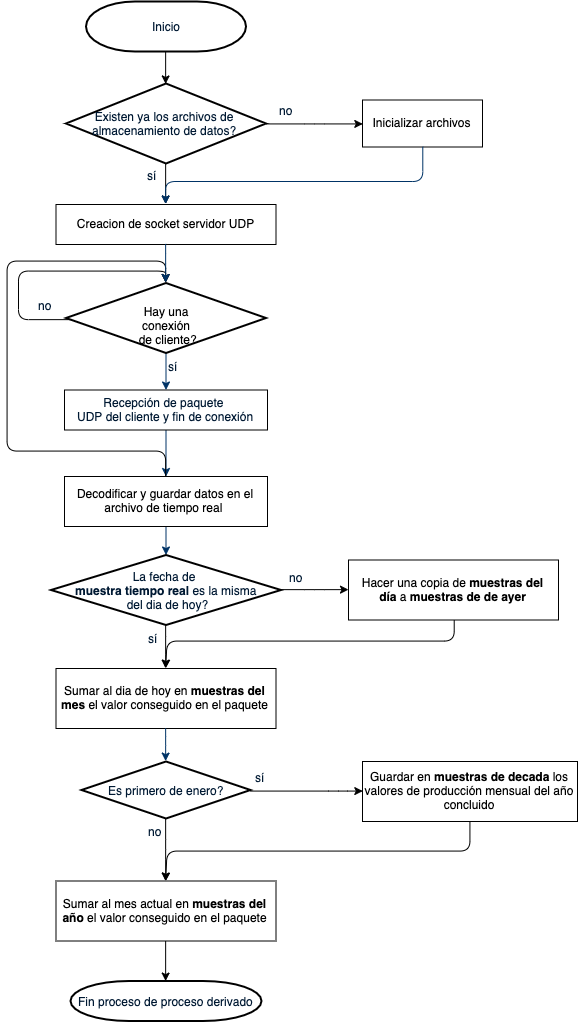
\includegraphics[scale=.5]{Capitulo5/images/logica_server_udp.png}
	\caption{Lógica del programa del servidor del microcontrolador}
	\label{fig:programa del servidor microcontrolador}
\end{figure} 

\subsubsection{Pruebas}
\textbf{Tipo :} Unitaria de Funcionalidad \\ \newline

Para poder comprobar su funcionamiento, redirigimos los paquetes del programa del microcontrolador hacia la IP y puerto 4000 UDP del servidor, teniendo como resultado en consola lo que se muestra en la figura \ref{fig:consola server udp}, donde se muestran las conexiones del microcontrolador, estos mensajes llegan aproximadamente cada segundo más décimas de segundo.

\begin{figure}[H]
	\centering
	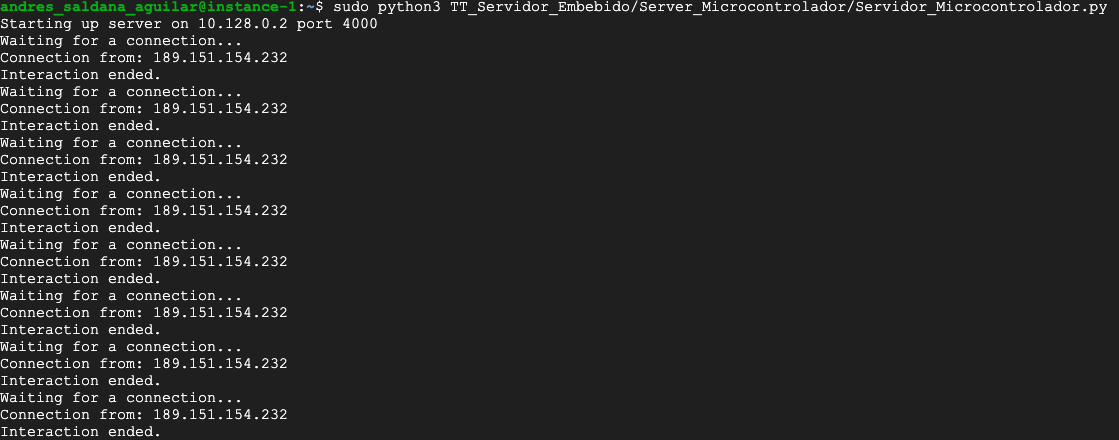
\includegraphics[scale=.3]{Capitulo5/images/udp_server_console.png}
	\caption{Salida de consola del servicio servidor UDP}
	\label{fig:consola server udp}
\end{figure} 

Los archivos que consume este servicio dan como resultado lo mostrado en las siguientes imágenes.

\begin{figure}[H]
	\centering
	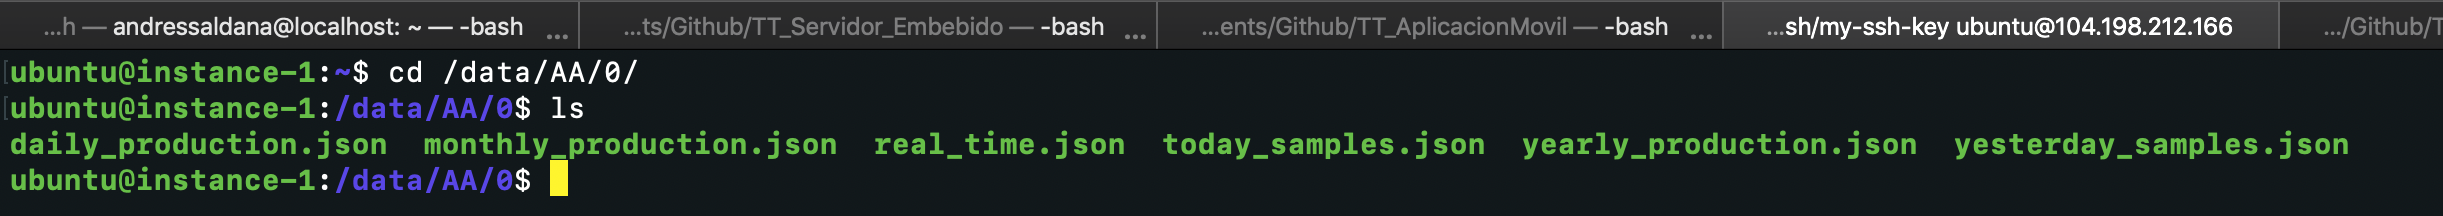
\includegraphics[scale=.3]{Capitulo5/images/dirlist.png}
	\caption{Listado de archivos creados por el servicio de de captura}
	\label{fig:}
\end{figure} 

\begin{figure}[H]
	\centering
	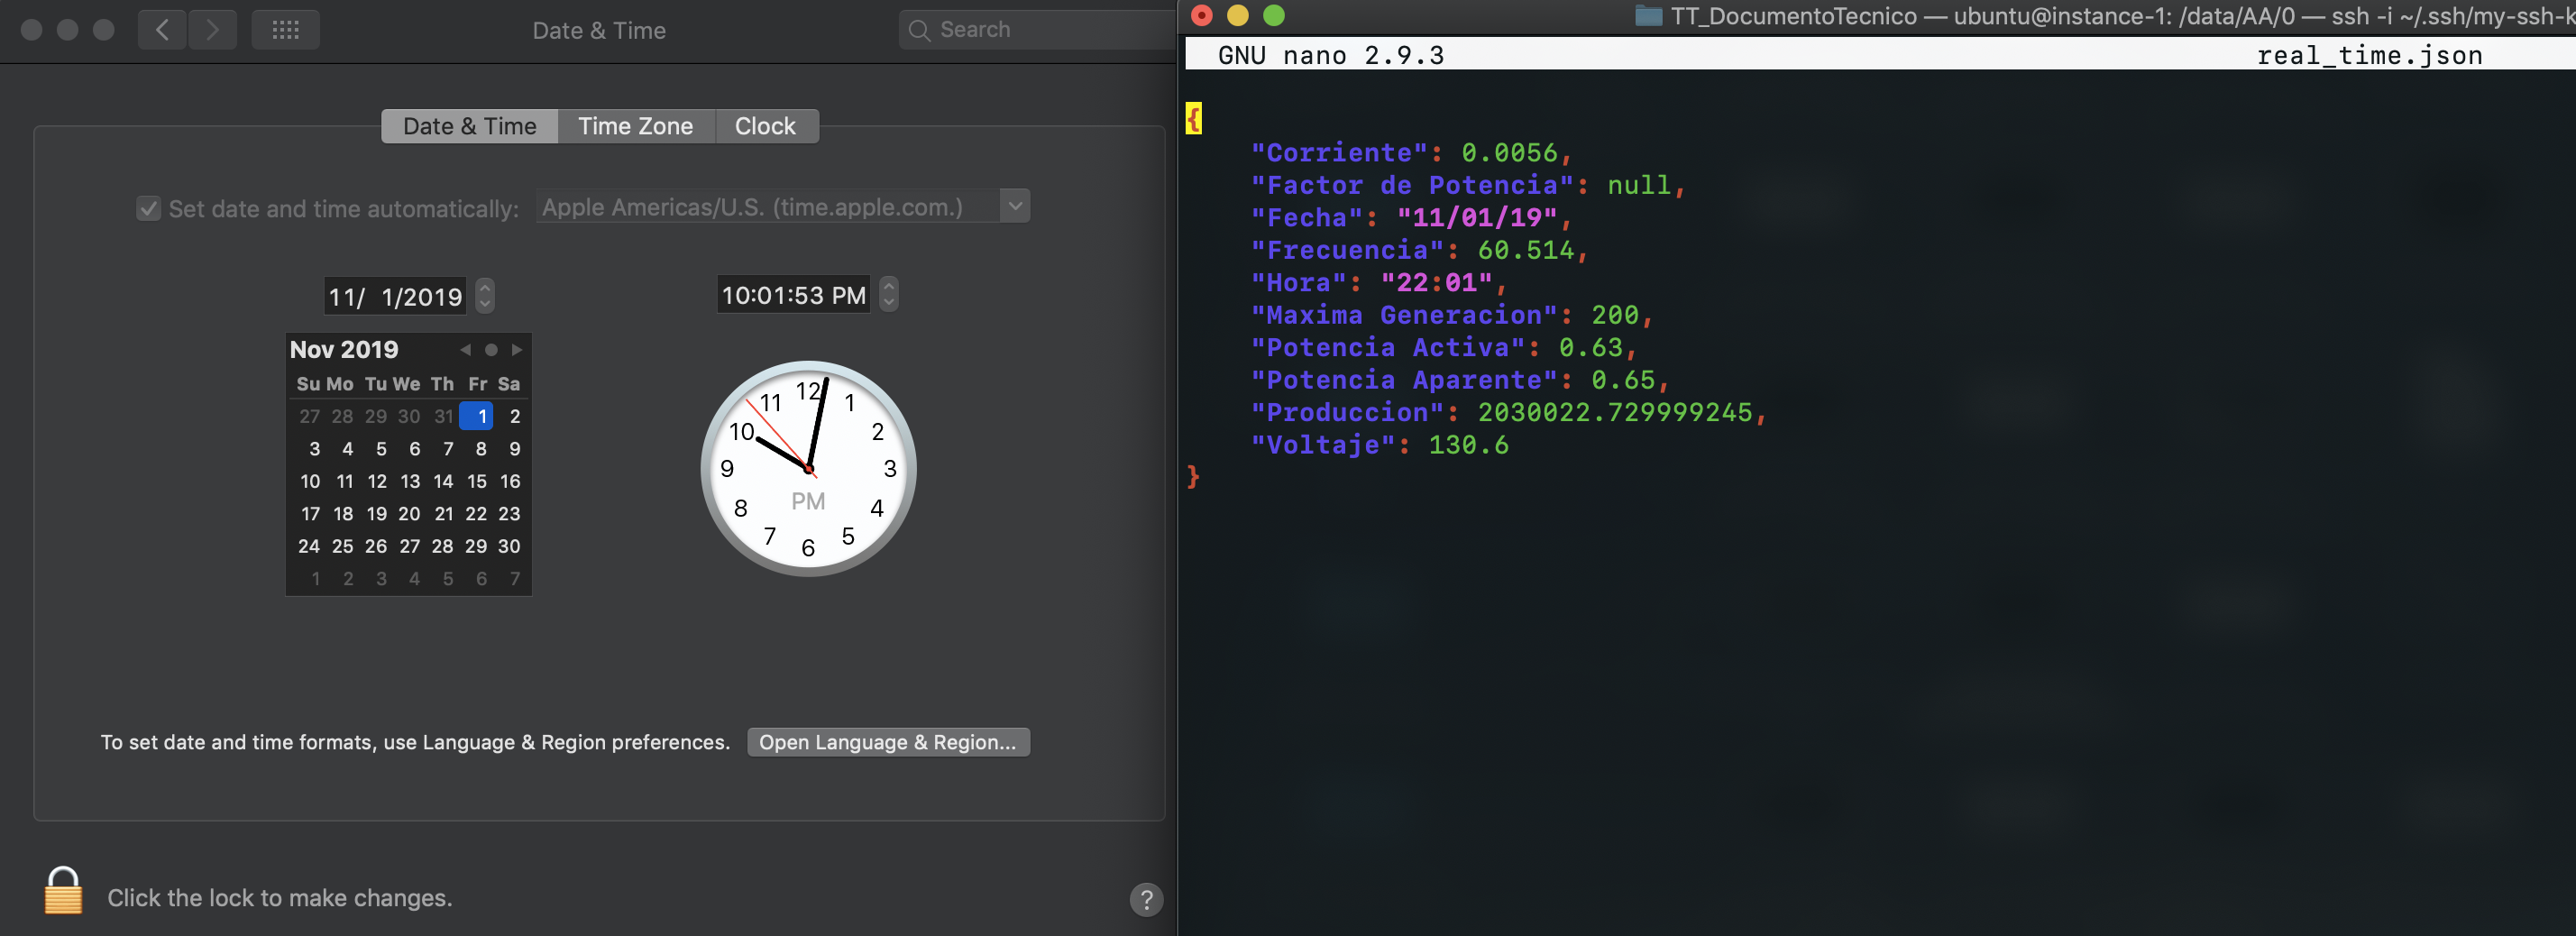
\includegraphics[scale=.3]{Capitulo5/images/real_time.png}
	\caption{Archivo con la muestra de tiempo real}
	\label{fig:}
\end{figure} 

\begin{figure}[H]
	\centering
	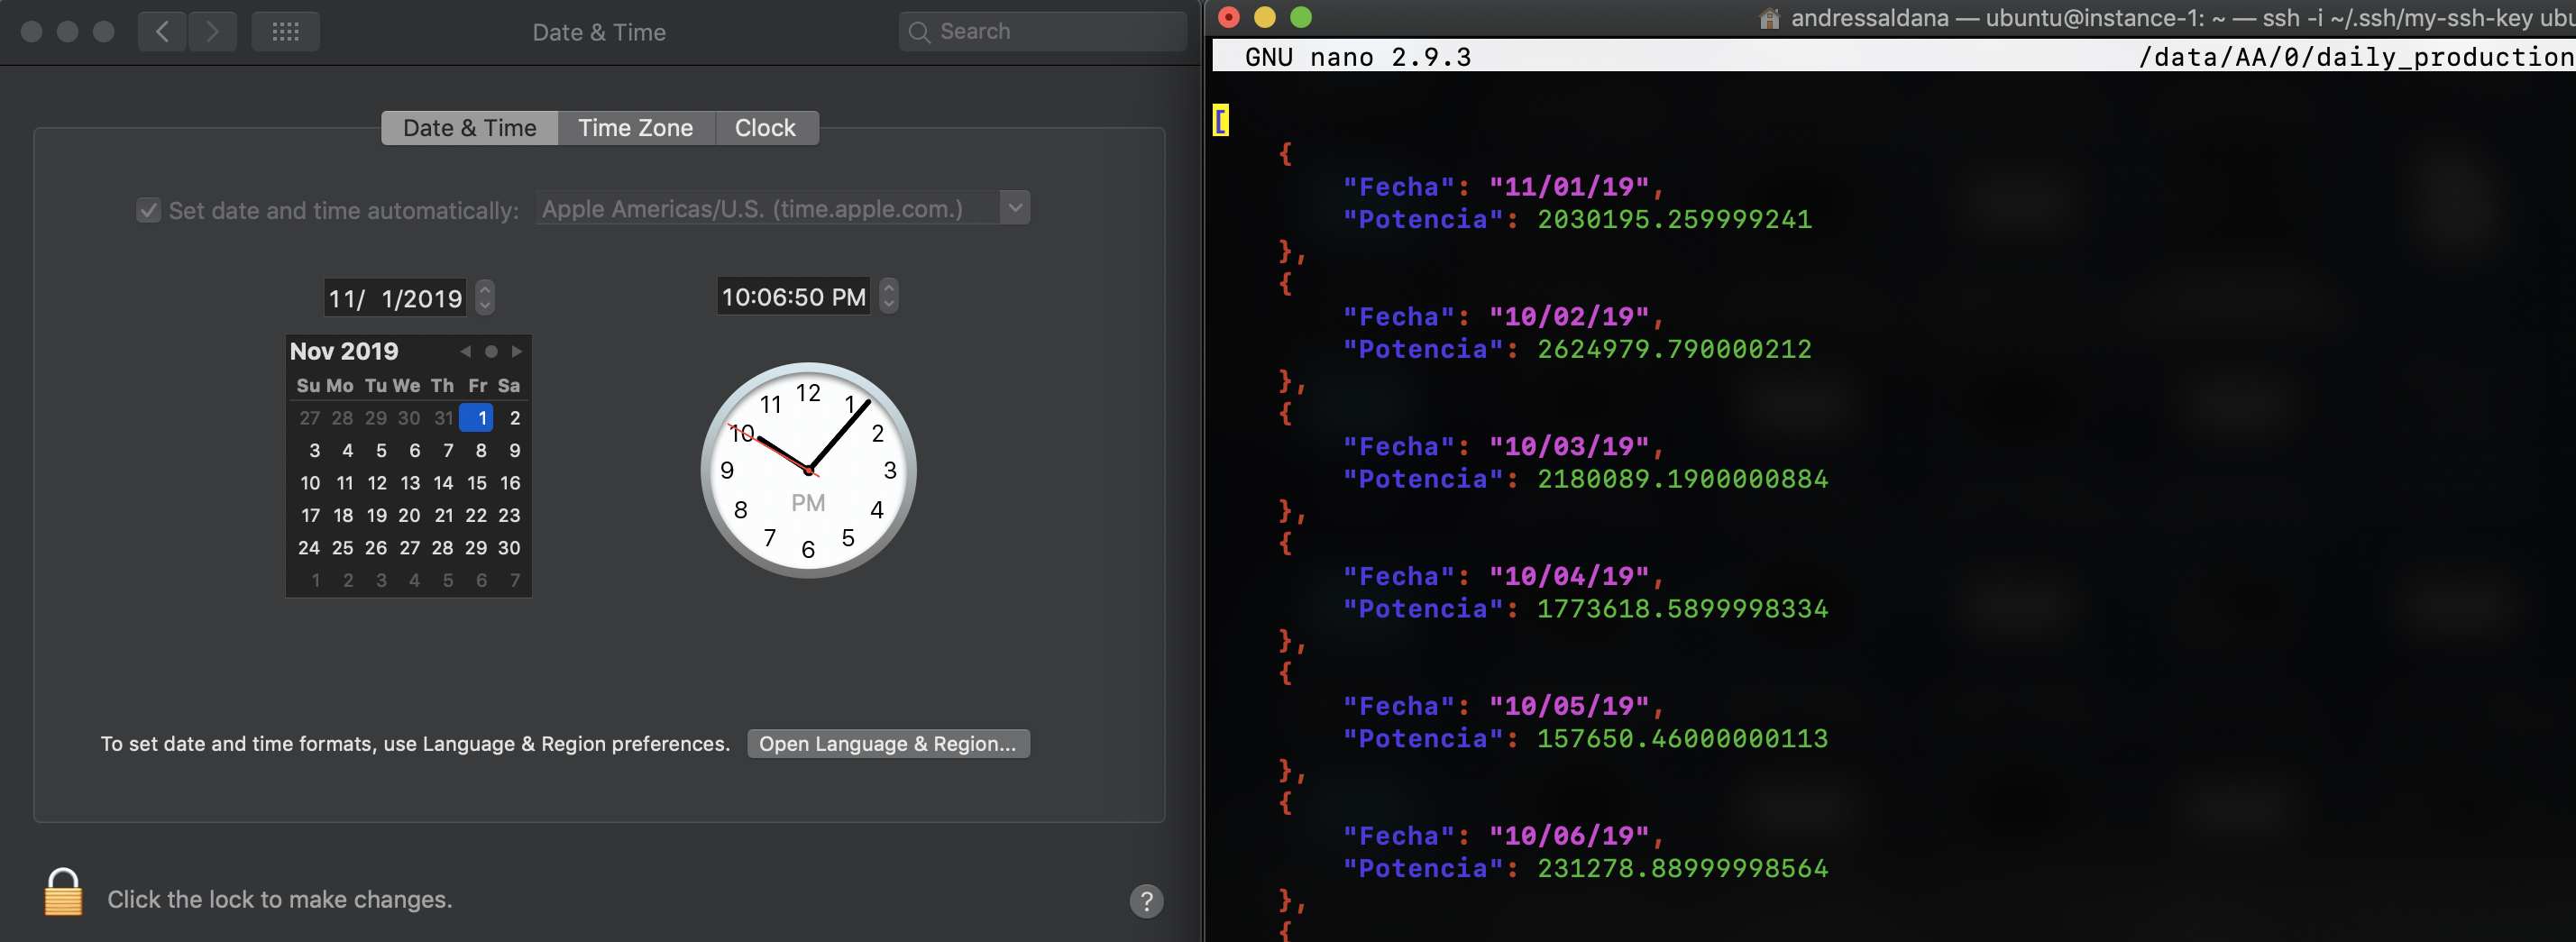
\includegraphics[scale=.3]{Capitulo5/images/daily.png}
	\caption{Extracto de las 31 muestras de producción de energía acumulada por cada día de un mes}
	\label{fig:}
\end{figure}

\begin{figure}[H]
	\centering
	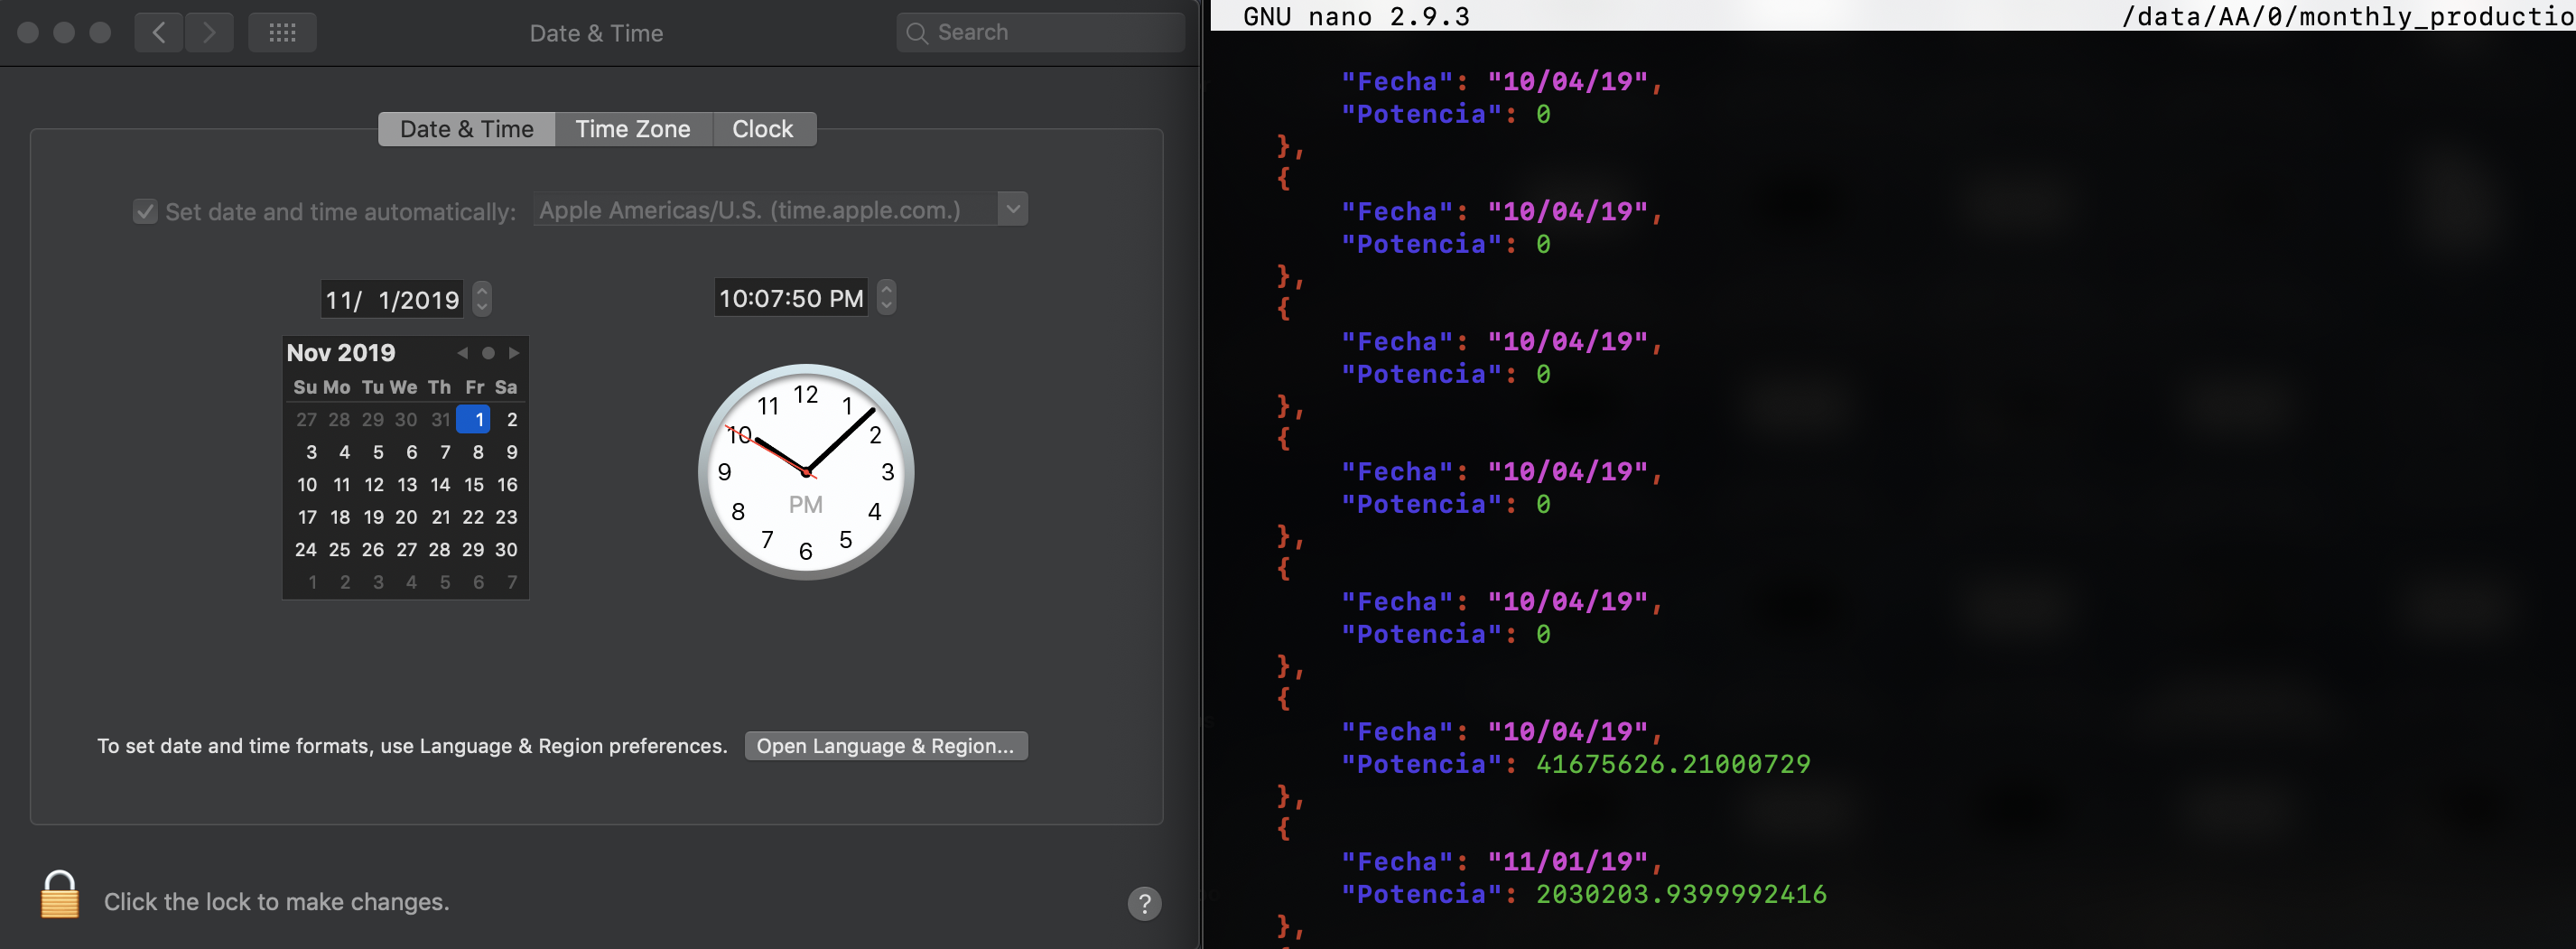
\includegraphics[scale=.3]{Capitulo5/images/monthly.png}
	\caption{Extracto de las 12 muestras de producción de energía acumulada por cada mes del año}
	\label{fig:}
\end{figure} 


\begin{figure}[H]
	\centering
	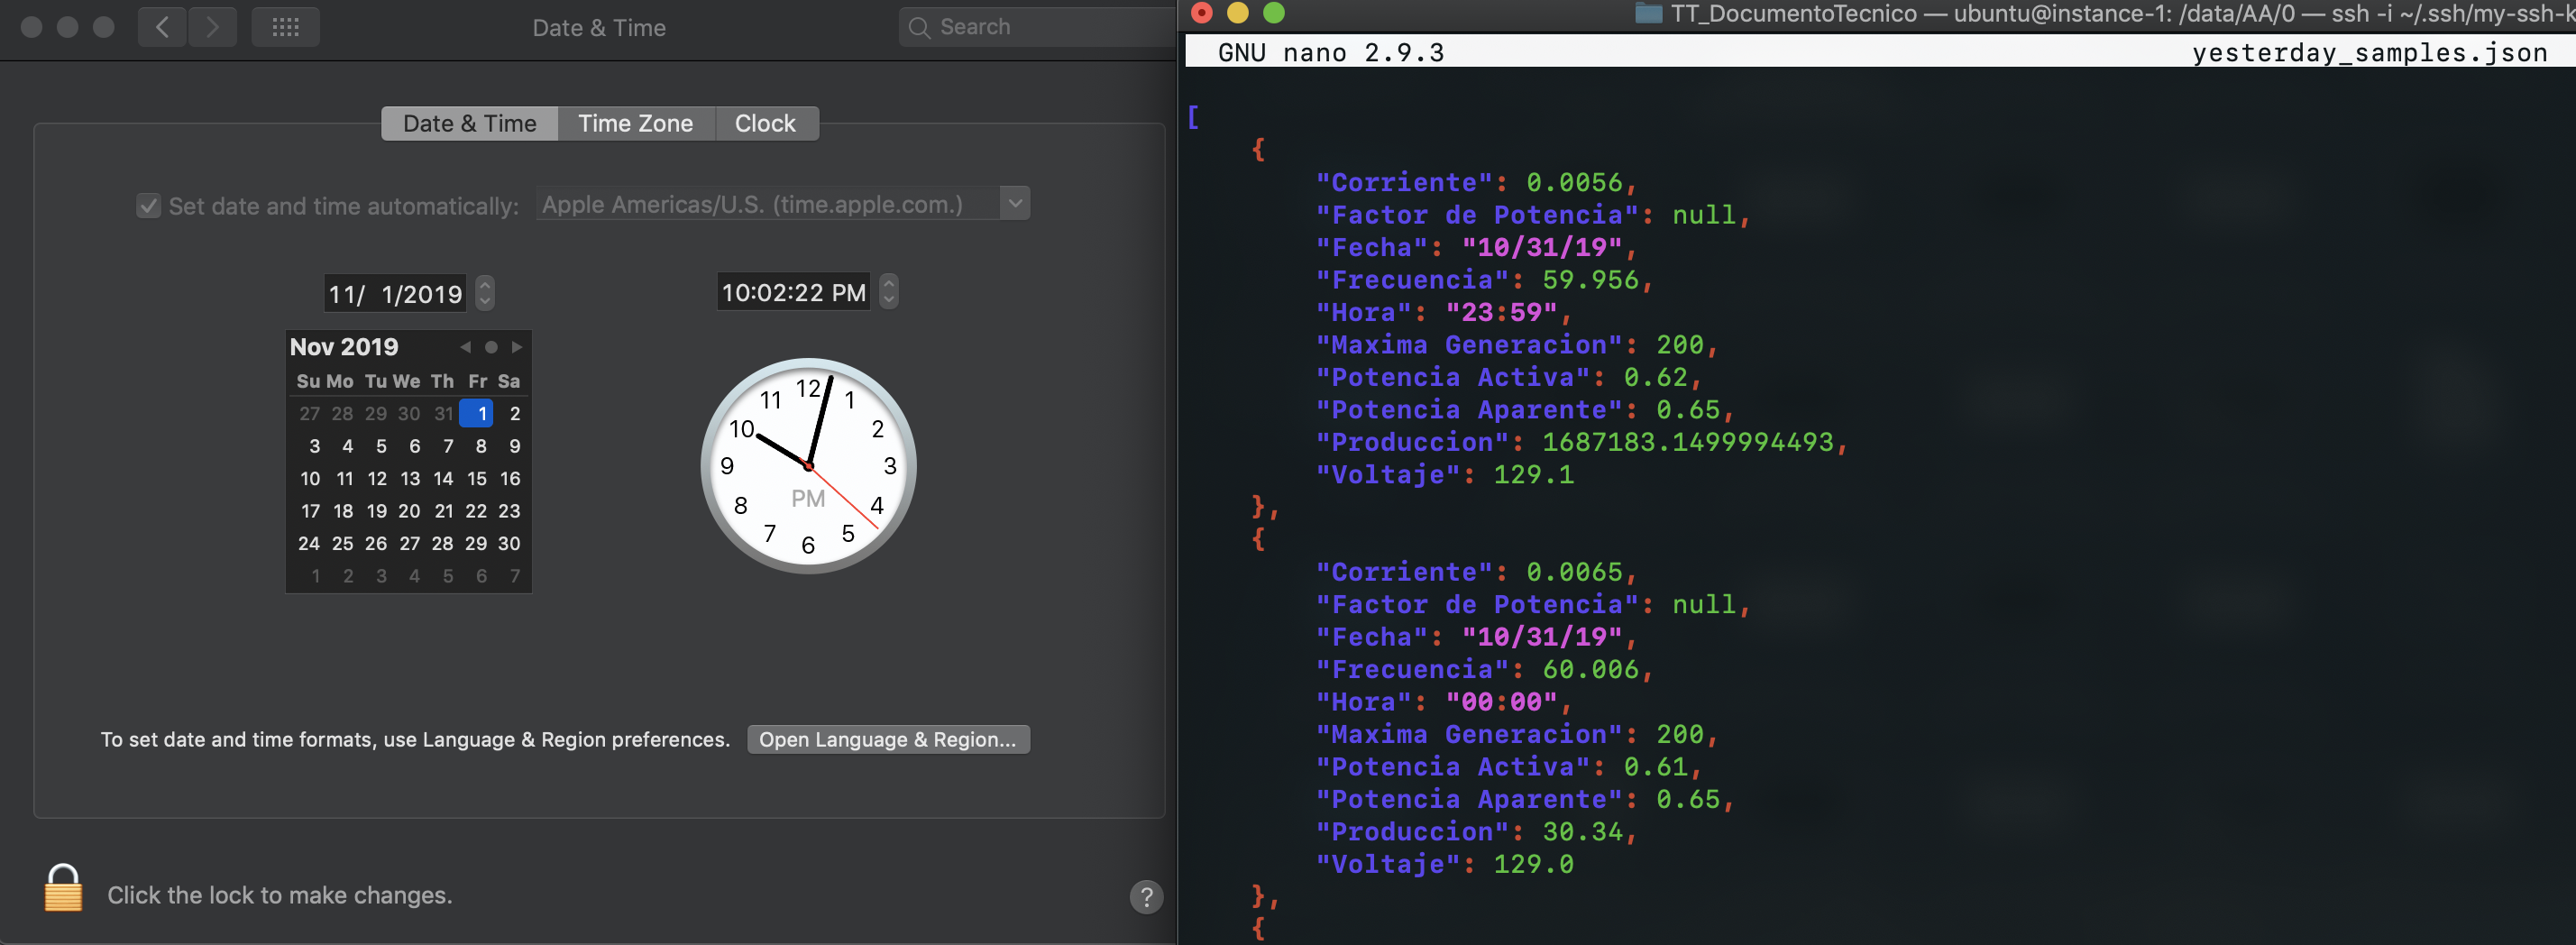
\includegraphics[scale=.3]{Capitulo5/images/yesterday.png}
	\caption{Extracto del archivo de 1440 con las muestras de producción de energía para la gráfica de cada minuto del día de ayer}
	\label{fig:}
\end{figure} 

\subsubsection{Pruebas}
\textbf{Tipo :} De Carga
\\ \newline

Una prueba primordial en este sistema que consta de una red de sensores, es conocer cuantos nodos sensores soporta el servidor embebido, por lo que utilizamos una herramienta de prueba de cargas hacia el servidor llamada JMeter \citep{JMeter}, a continuación se describe como se realizo esta prueba.

Indicar cuantas peticiones simultaneas se realizarán en un lapso de tiempo, en la figura \ref{fig:threadgroup} indicamos que se realizaran 1950 en 2 minutos y medio, es decir, 13 nodos enviando información cada segundo, elegimos que la prueba durara este tiempo porque el comportamiento se vuelve constante después de un minuto.

\begin{figure}[H]
	\centering
	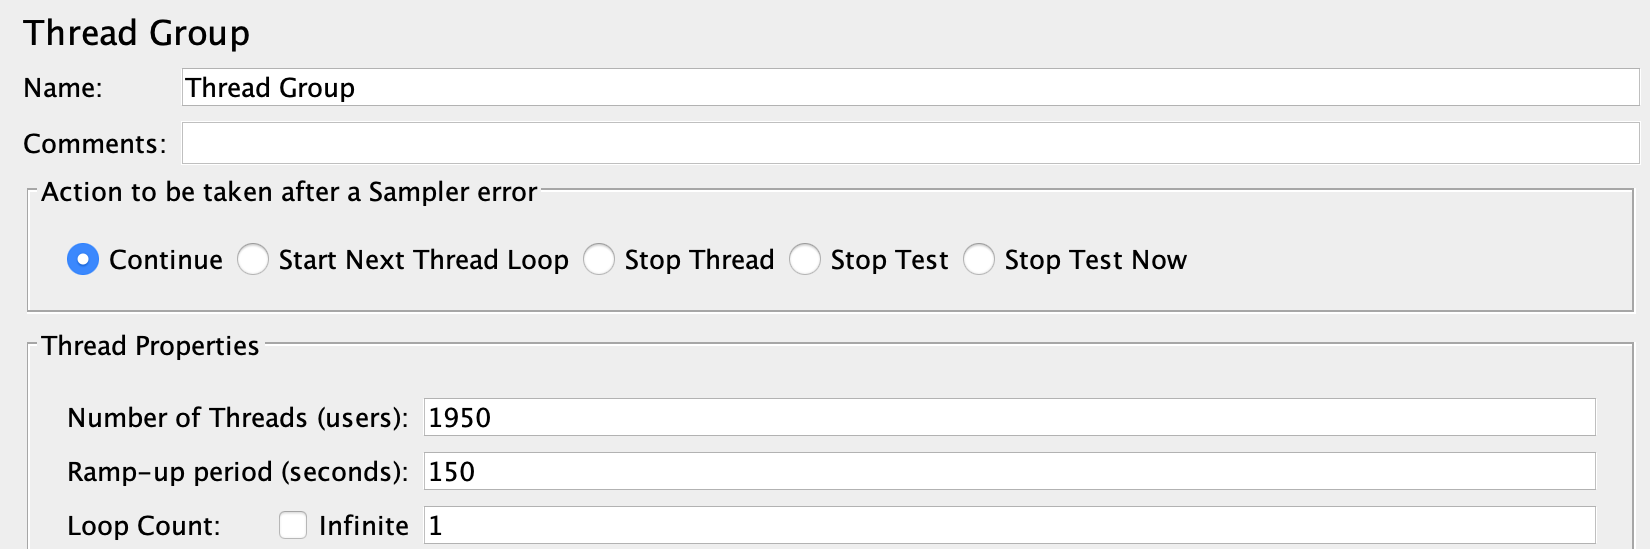
\includegraphics[scale=.3]{Capitulo5/images/tread_group.png}
	\caption{Configuración en JMeter de grupo de hilos}
	\label{fig:threadgroup}
\end{figure} 

Esta cifra se escogió porque realizando pruebas con distintas cargas, descubrimos que con esta frecuencia de actividad el sistema mantiene su rendimiento constante en el tiempo sin fallar \ref{fig:udpsummary}, al tratarse de comunicación UDP, no podemos contar con la respuesta de servidor, por lo que mandamos el valor de uno como valor de potencia activa, de manera que si mandamos un total de 1950 muestras, debe guardarse esa cantidad menos uno (porque el contador inicia en cero) en el servidor como la producción acumulada como se muestra en la figura \ref{fig:udptestjson} teniendo como tiempo de conexión promedio menor a los 3ms \ref{fig:udpconnect}.

\begin{figure}[H]
	\centering
	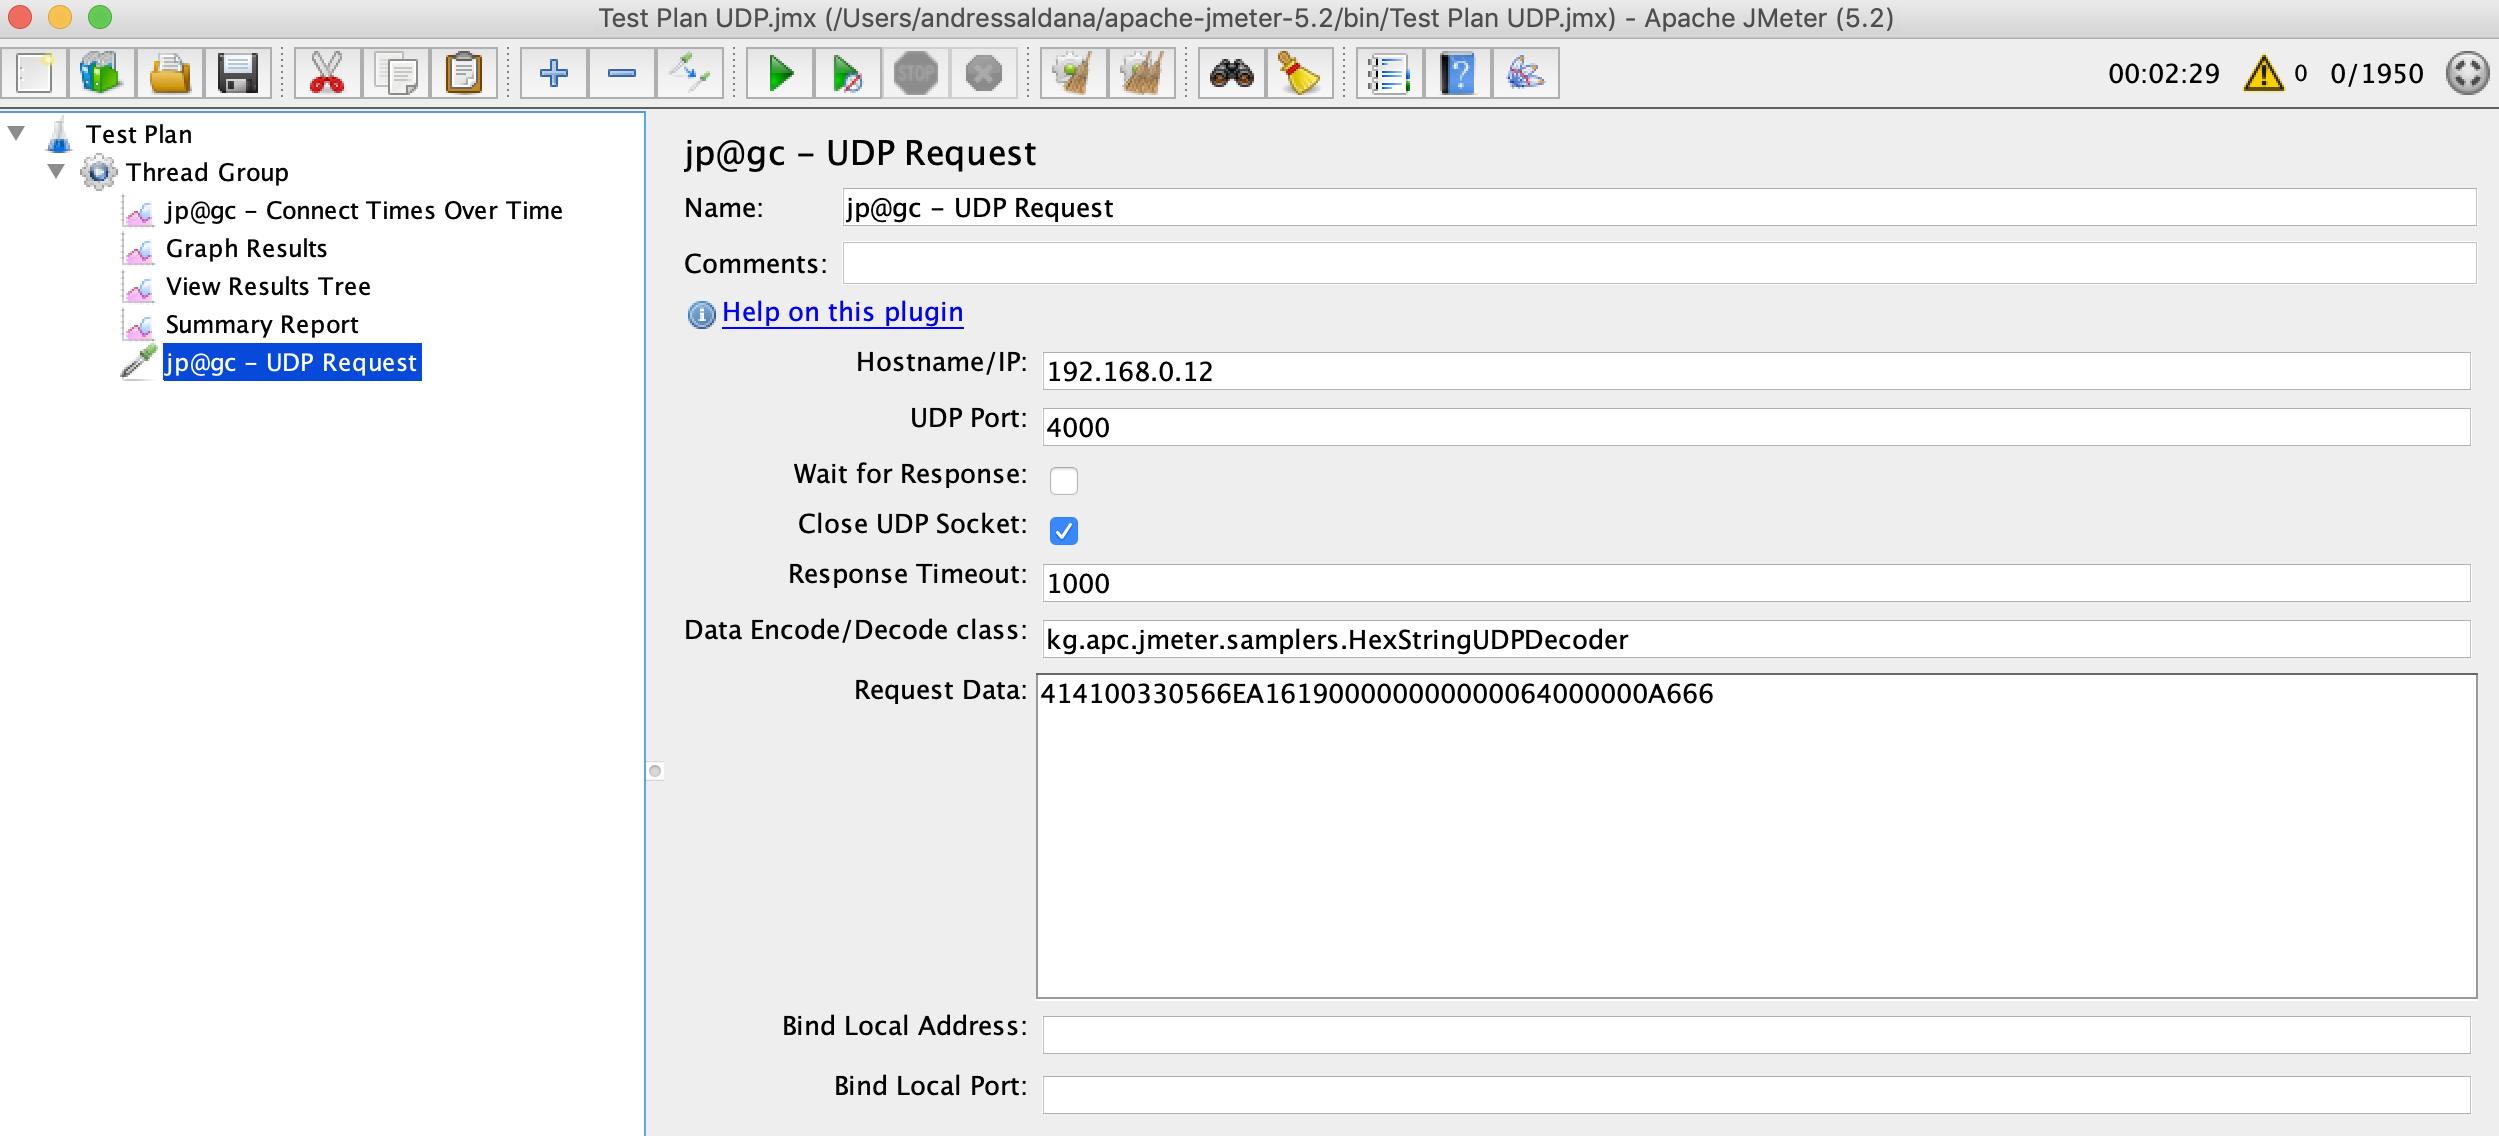
\includegraphics[scale=.3]{Capitulo5/images/udp_test_config.png}
	\caption{Configuración en JMeter de IP, puerto y mensaje a enviar en valor Hexadecimal}
	\label{fig:uddpconfig}
\end{figure} 

\begin{figure}[H]
	\centering
	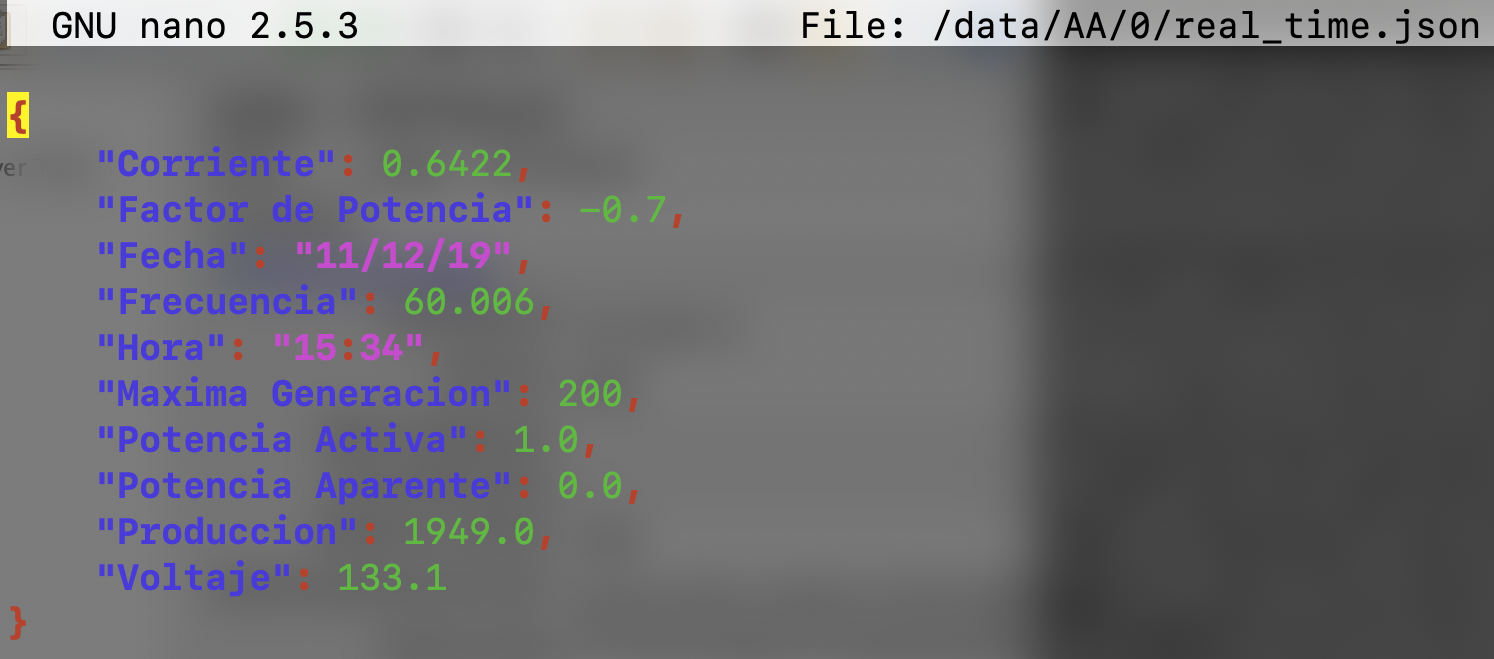
\includegraphics[scale=.5]{Capitulo5/images/udp_test_production.png}
	\caption{Producción acumulada durante la prueba en el servidor}
	\label{fig:udptestjson}
\end{figure} 

\begin{figure}[H]
	\centering
	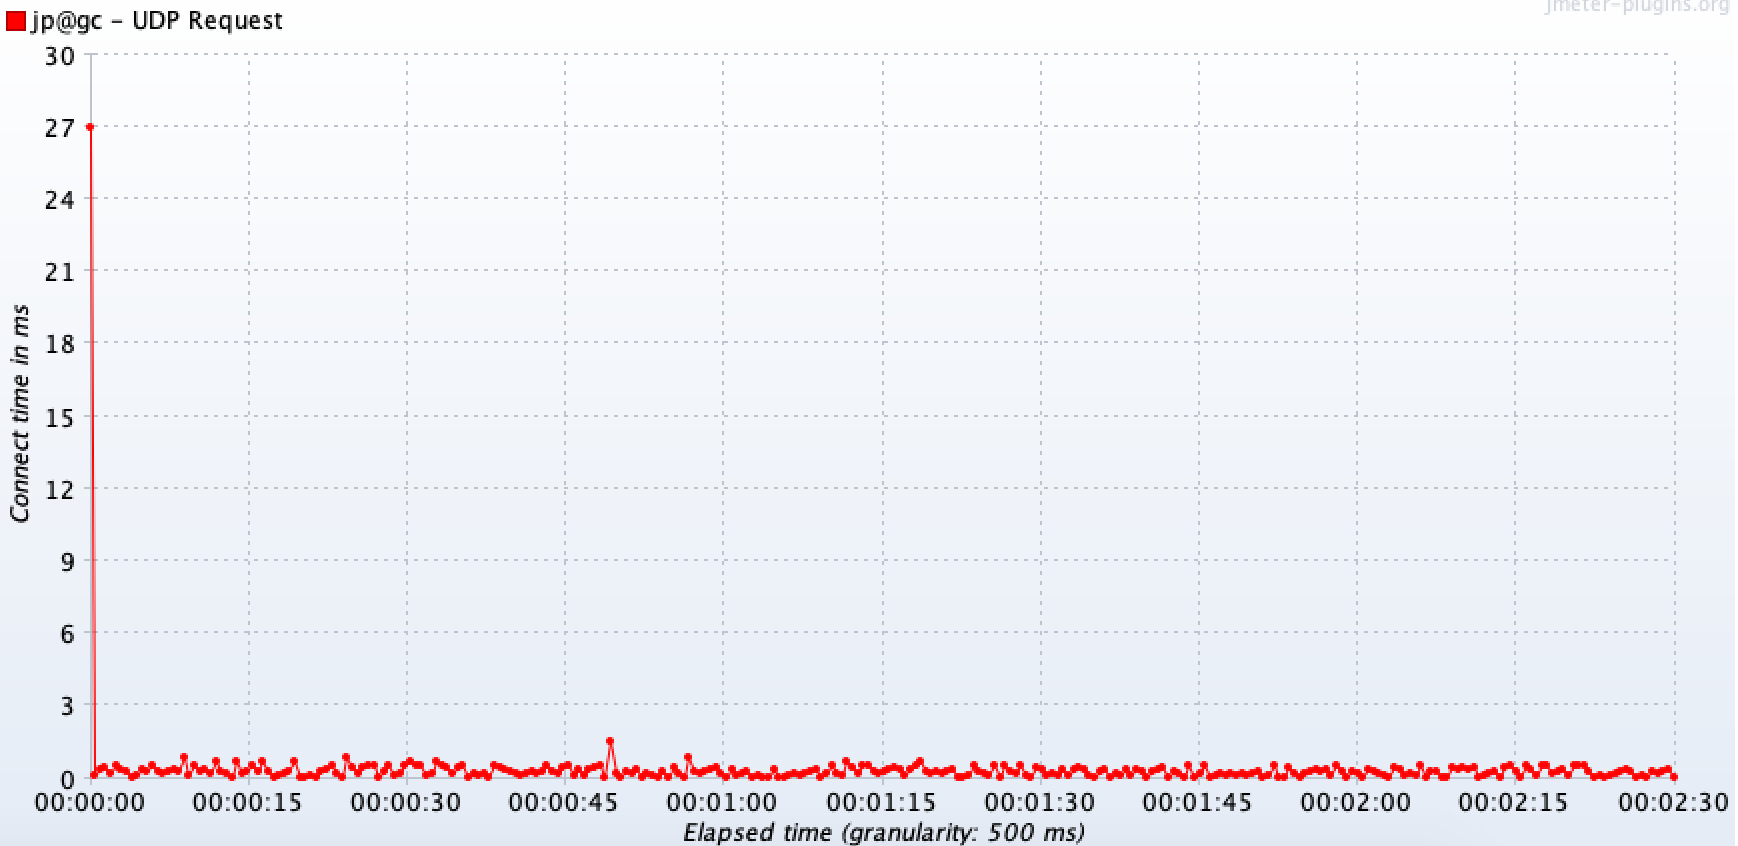
\includegraphics[scale=.3]{Capitulo5/images/udp_test_connect.png}
	\caption{Gráfica de tiempo de conexión en el tiempo de prueba}
	\label{fig:udpconnect}
\end{figure} 

\begin{figure}[H]
	\centering
	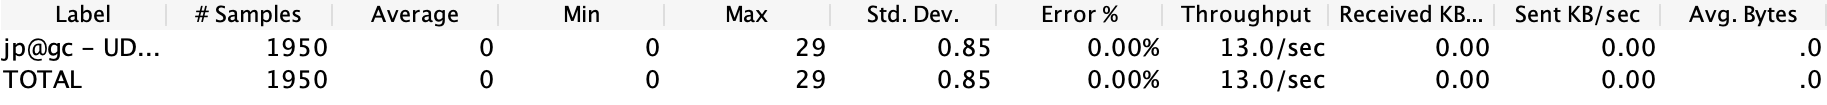
\includegraphics[scale=.5]{Capitulo5/images/udp_test_summary.png}
	\caption{Resumen de la prueba realizada}
	\label{fig:udpsummary}
\end{figure} 

\subsection{Implementando el servicio de creación de muestras para  gráficas del día actual}

\subsubsection{Desarrollo}

Identificamos que lo mas conveniente sería independizar este proceso de la captura de paquetes para con el propósito de modularizar el sistema y lograr un bajo acoplamiento, implementando la lógica como se muestra en la figura \ref{fig:programa graficador}, la información de gráficas también se guarda en formato JSON, que nos permite hacer mas sencillo la compatibilidad con distintos lenguajes.

\begin{figure}[H]
	\centering
	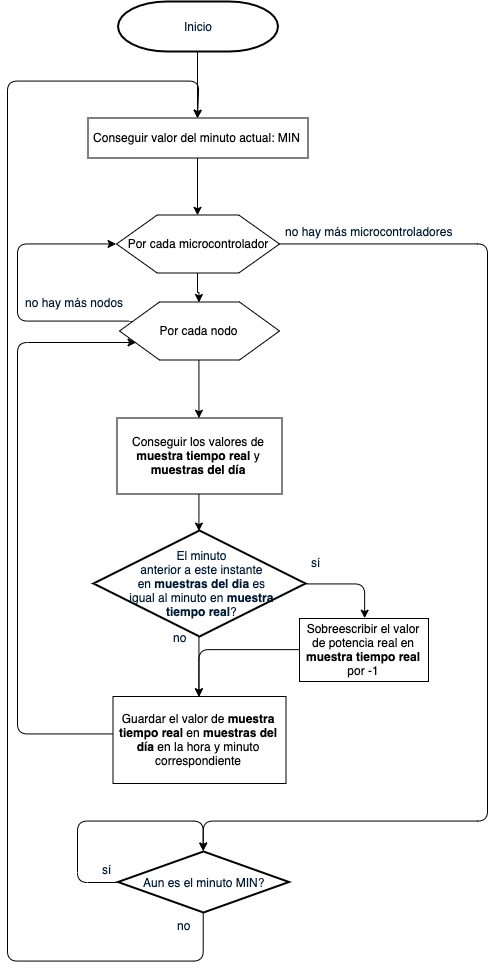
\includegraphics[scale=.5]{Capitulo5/images/logica_graficador.png}
	\caption{Lógica del programa graficador}
	\label{fig:programa graficador}
\end{figure} 

\subsubsection{Pruebas}
\textbf{Tipo :} Unitaria de Funcionalidad \\ \newline

El resultado de este programa se ve reflejado en los archivos de muestras diarias, como se muestra en la figura \ref{fig:muestras diarias}.

\begin{figure}[H]
	\centering
	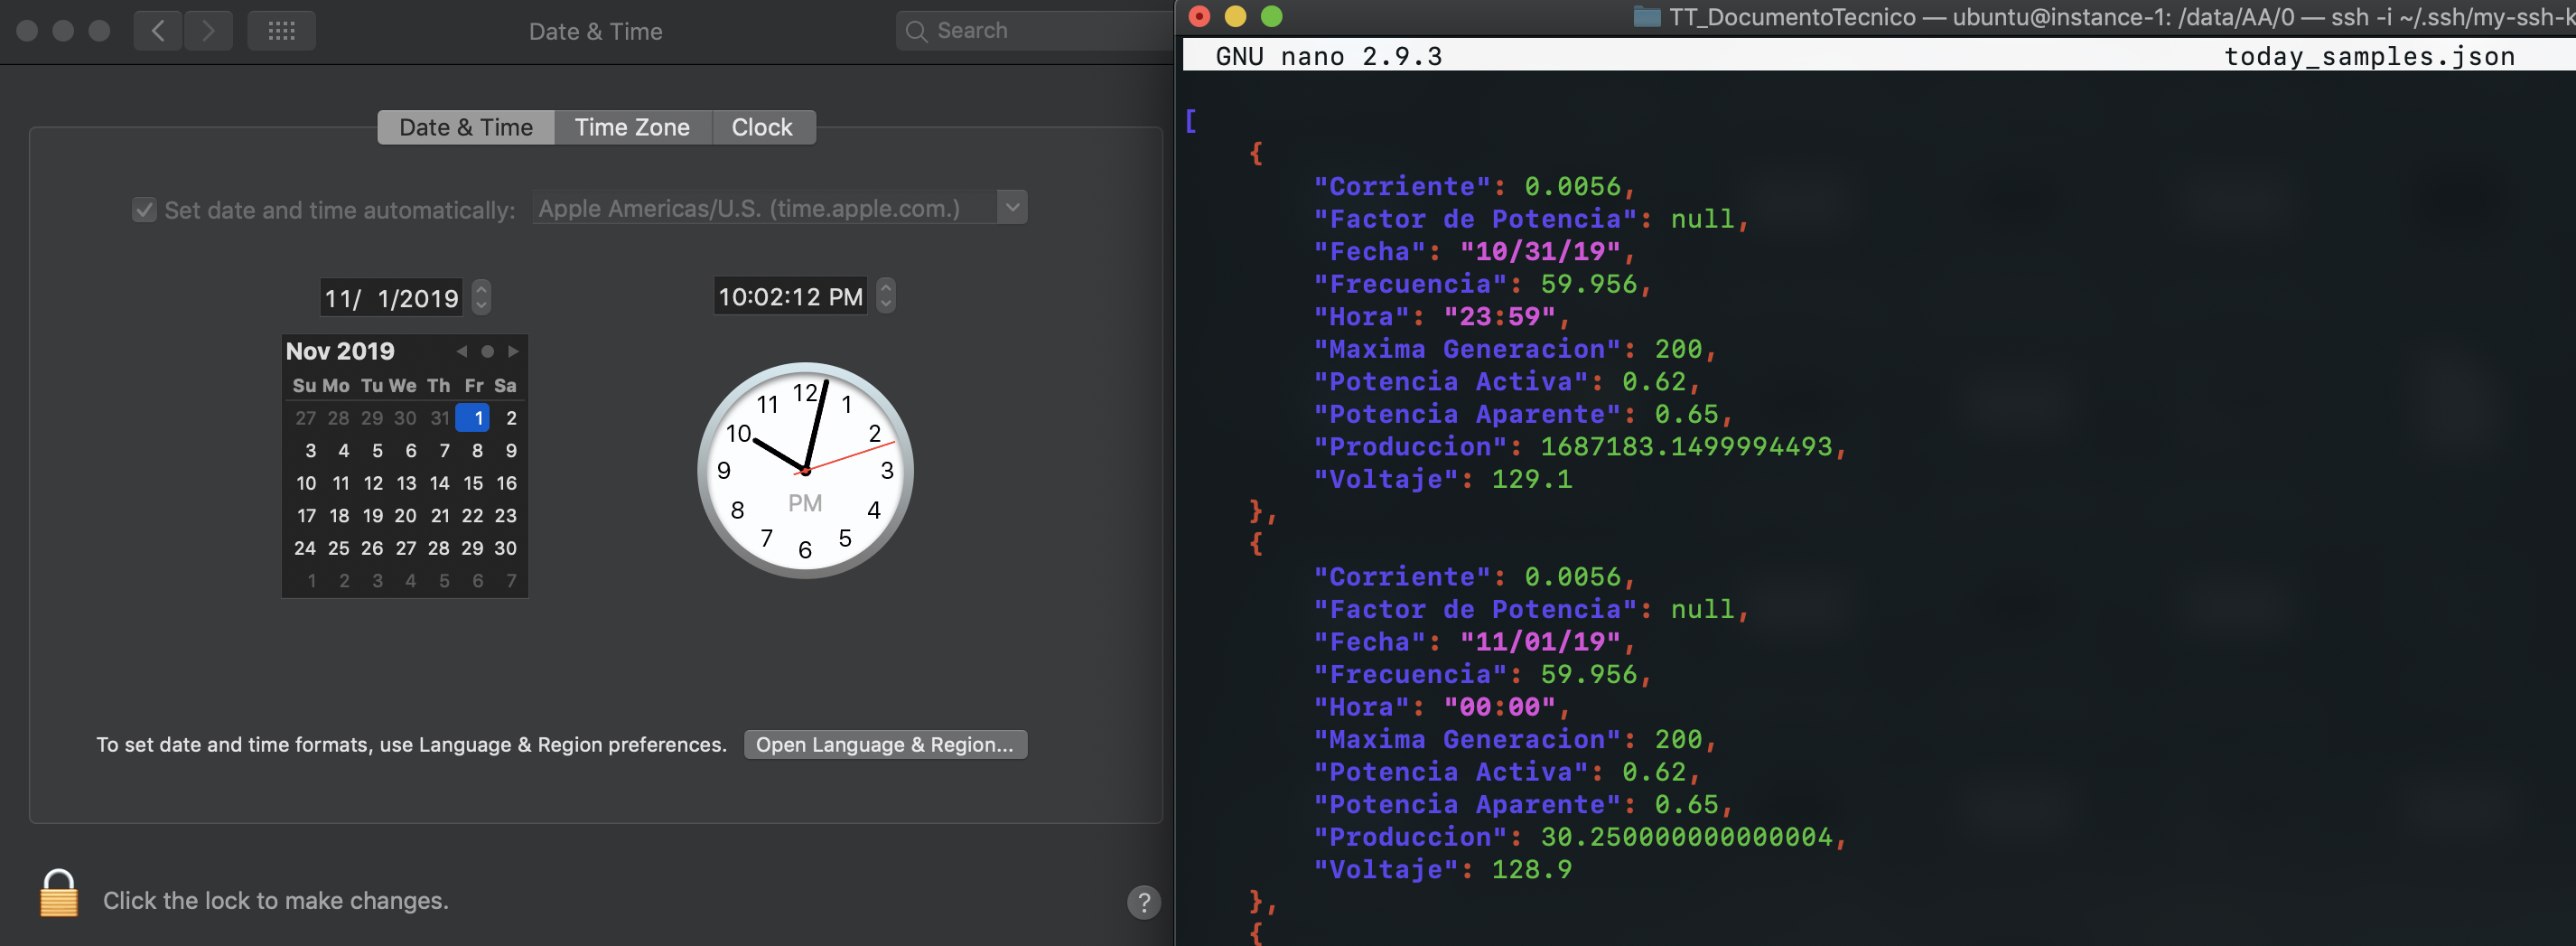
\includegraphics[scale=.3]{Capitulo5/images/today.png}
	\caption{Extracto del archivo de 1440 con las muestras de producción de energía para la gráfica de cada minuto del día de hoy}
	\label{fig:muestras diarias}
\end{figure} 

\subsection{Implementando el servicio de atención a clientes de aplicación móvil}

\subsubsection{Desarrollo}

Este servicio esta implementado en el lenguaje de programación Python en su versión 3.0, su propósito es atender las peticiones provenientes de la aplicación móvil como indica el caso de uso \ref{SUB-M-CU1.10}, elaboramos un diagrama de flujo para simplificar la explicación de la lógica del programa \ref{fig:programa del servidor aplicacion}, también hicimos uso de la duplicación de procesos para aumentar el rendimiento del programa, este programa corre como un servicio en nuestro servidor Linux.

\begin{figure}[H]
	\centering
	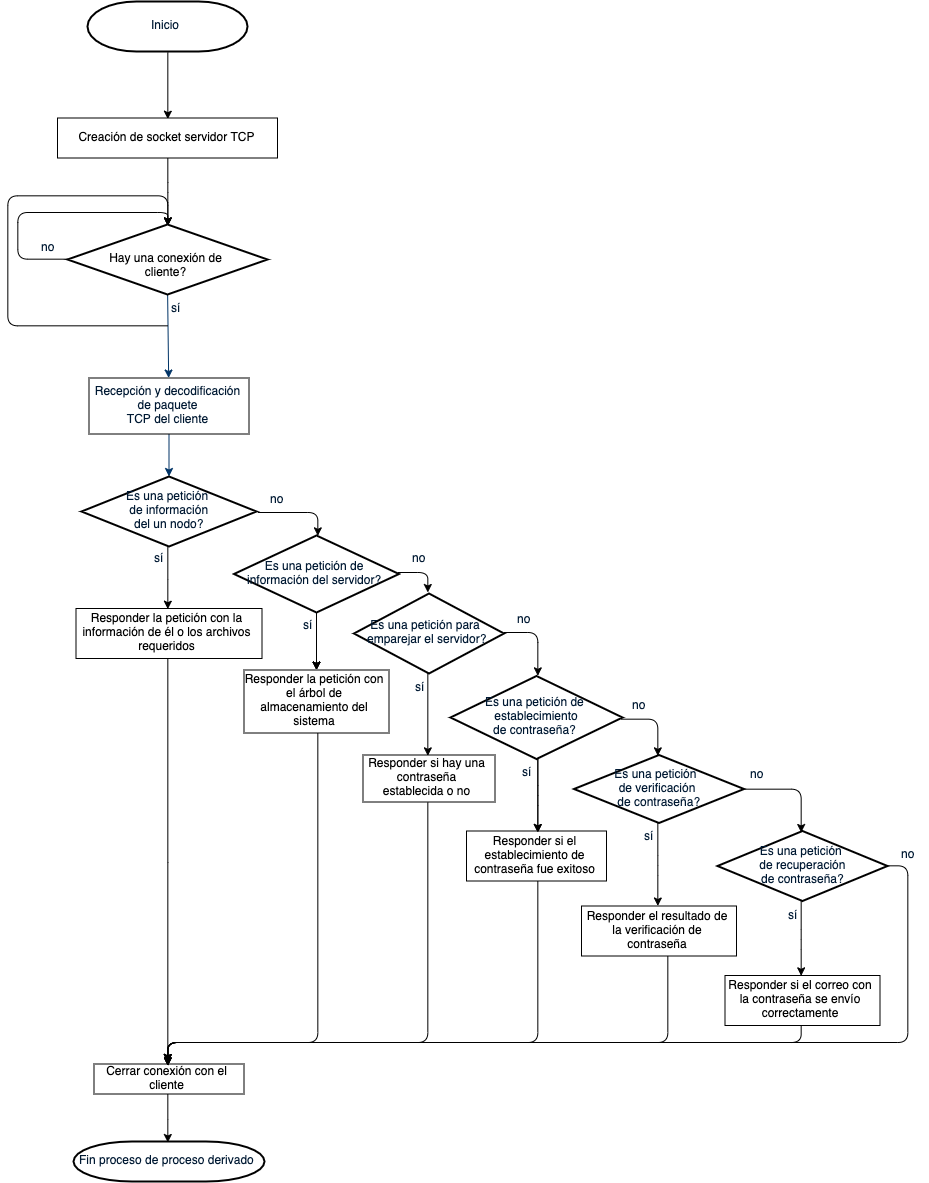
\includegraphics[scale=.4]{Capitulo5/images/logica_server_tcp.png}
	\caption{Lógica del programa del servidor de la aplicación}
	\label{fig:programa del servidor aplicacion}
\end{figure} 

\subsubsection{Pruebas}
\textbf{Tipo :} Unitaria de Funcionalidad \\ \newline

Para probar su funcionamiento, se realizaron las peticiones posibles hacia el servidor:

Comando: \hl{getdata AA 0 realtime}
\begin{figure}[H]
	\centering
	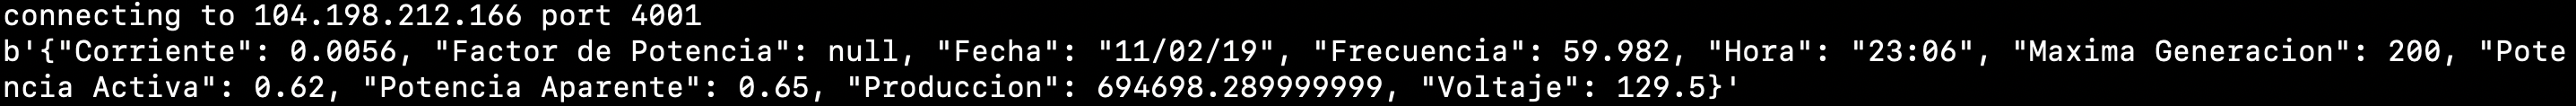
\includegraphics[scale=.3]{Capitulo5/images/get_data.png}
	\caption{Respuesta del comando para conseguir la información del el archivo de tiempo real}
	\label{fig:}
\end{figure} 

Comando: \hl{getinfo}
\begin{figure}[H]
	\centering
	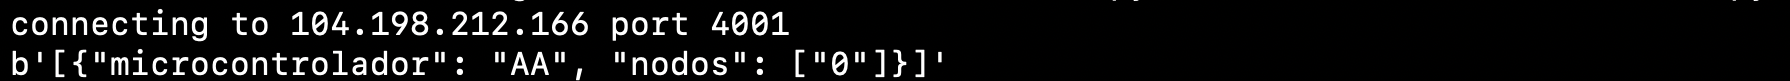
\includegraphics[scale=.5]{Capitulo5/images/get_info.png}
	\caption{Respuesta del comando que trae la información del árbol de información del servidor}
	\label{fig:}
\end{figure} 

Comando: \hl{connect}
\begin{figure}[H]
	\centering
	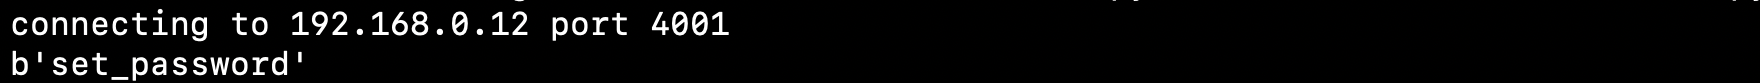
\includegraphics[scale=.5]{Capitulo5/images/connect.png}
	\caption{Respuesta a conocer si el servidor tiene ya una contraseña, nos indica que no hay contraseña}
	\label{fig:}
\end{figure} 

\begin{figure}[H]
	\centering
	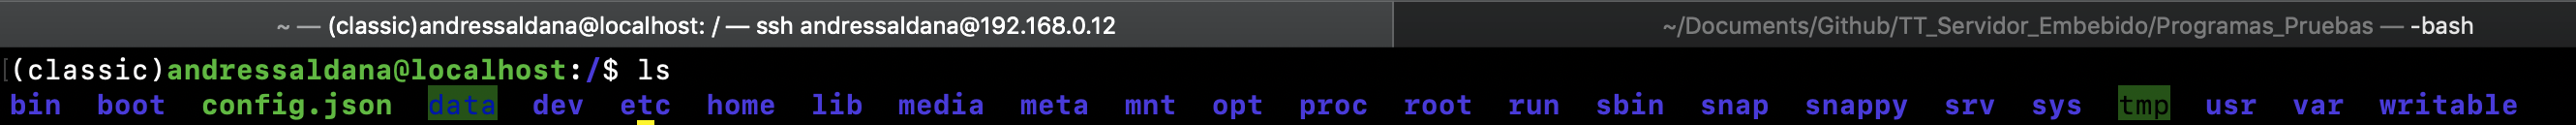
\includegraphics[scale=.35]{Capitulo5/images/listconfig.png}
	\caption{Ubicación del archivo de configuración, en el directorio raíz con el nombre de config.json}
	\label{fig:}
\end{figure} 

\begin{figure}[H]
	\centering
	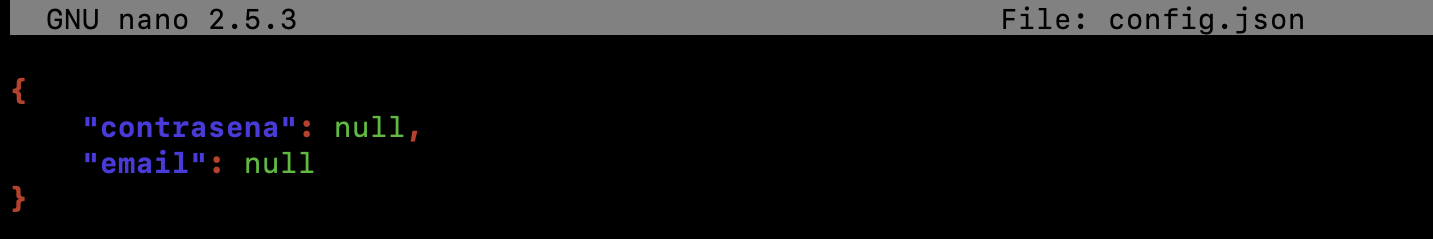
\includegraphics[scale=.5]{Capitulo5/images/nullconfig.png}
	\caption{Archivo de configuración con variables sin asignar}
	\label{fig:}
\end{figure} 

Comando: \hl{setpassword Secret1 smonitorp@gmail.com}
\begin{figure}[H]
	\centering
	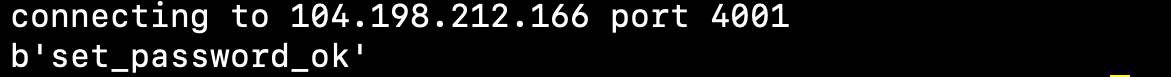
\includegraphics[scale=.5]{Capitulo5/images/set_password.png}
	\caption{Respuesta al comando que configura la contraseña}
	\label{fig:}
\end{figure} 

\begin{figure}[H]
	\centering
	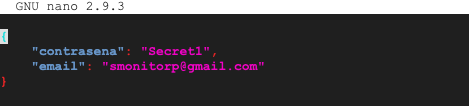
\includegraphics[scale=.6]{Capitulo5/images/setconfig.png}
	\caption{Archivo de configuración con variables asignadas después del setpassword}
	\label{fig:}
\end{figure} 

Comando: \hl{getpassword Secret1}
\begin{figure}[H]
	\centering
	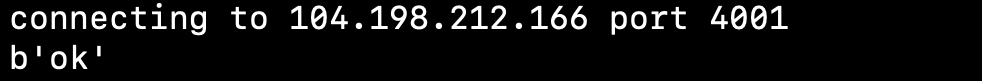
\includegraphics[scale=.5]{Capitulo5/images/forgot_pass.png}
	\caption{Respuesta a verificación de constraseña}
	\label{fig:}
\end{figure} 

Comando: \hl{forgotpassword}
\begin{figure}[H]
	\centering
	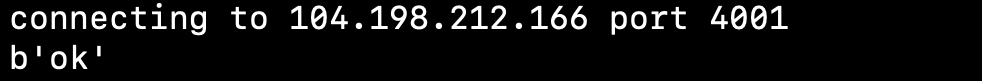
\includegraphics[scale=.5]{Capitulo5/images/forgot_pass.png}
	\caption{Respuesta del envió del correo, 'ok' si es exitoso, 'error' si el envió fue fallido}
	\label{fig:}
\end{figure} 

\begin{figure}[H]
	\centering
	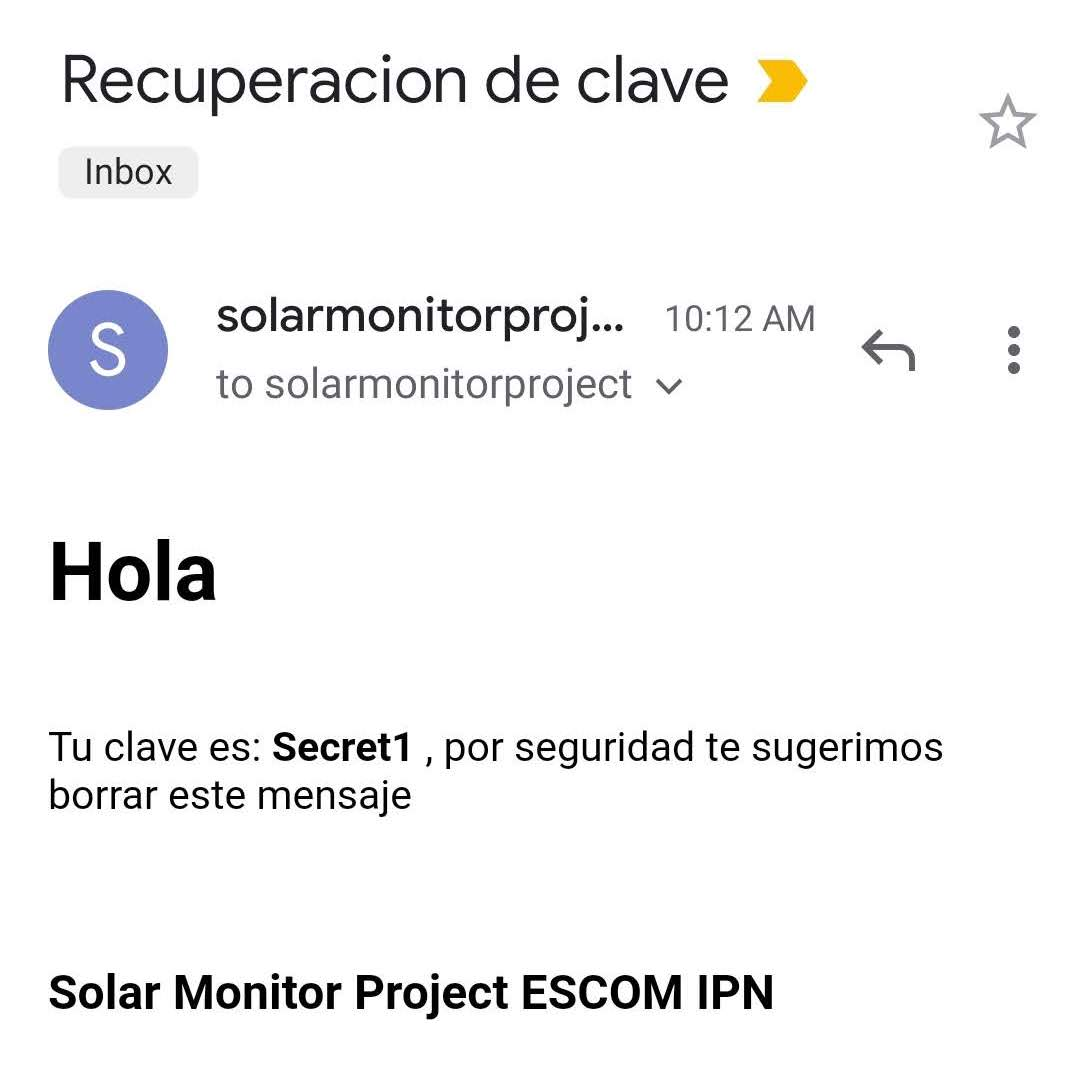
\includegraphics[scale=.2]{Capitulo5/images/correo.jpg}
	\caption{Correo resultado del comando forgotpassword}
	\label{fig:}
\end{figure}

\subsubsection{Pruebas}
\textbf{Tipo :} De carga \\ \newline

Una vez más, al tratarse de una red de sensores, probaremos cuantos usuarios podemos atender y cuantos nodos pueden tener en su aplicación, utilizaremos una vez más JMeter \citep{JMeter} para ello, a continuación se describe como se realizo esta prueba.

Indicar cuantas peticiones simultaneas se realizarán en un lapso de tiempo, en la figura \ref{fig:threadgroup} indicamos que se realizaran 1950 en 2 minutos y medio, es decir, 13 nodos enviando información cada segundo, elegimos que la prueba durara este tiempo porque el comportamiento se vuelve constante después de un minuto una vez más.

\begin{figure}[H]
	\centering
	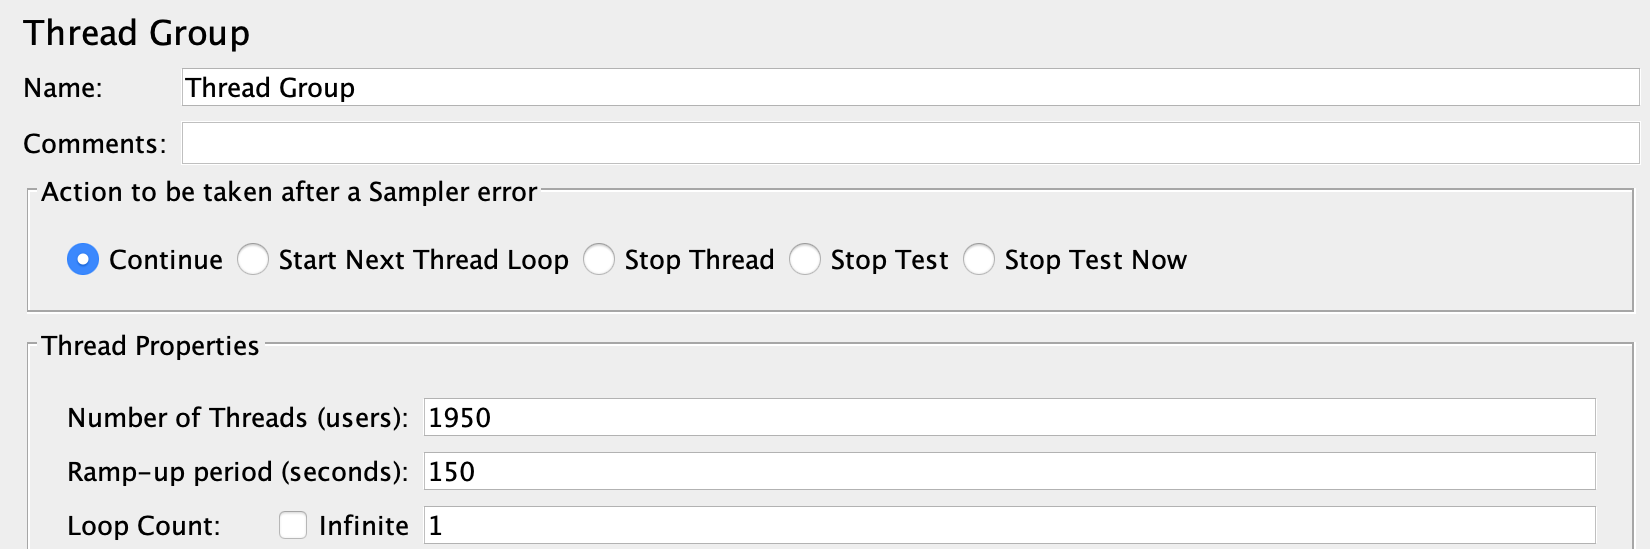
\includegraphics[scale=.3]{Capitulo5/images/tread_group.png}
	\caption{Configuración en JMeter de grupo de hilos}
	\label{fig:threadgroup}
\end{figure} 

Esta cifra se escogió porque realizando pruebas con distintas cargas, descubrimos que con esta frecuencia de actividad el sistema mantiene su rendimiento constante en el tiempo sin fallar \ref{fig:tcpsummary}, en este caso podemos conocer automáticamente si la petición fue exitosa y cuanto tardo gracias a que implementa el protocolo TCP, enviamos una petición para traer la información del archivo de tiempo real \ref{fig:tcpconfig}, que es el que se consulta para monitoreo cada 10 segundos esperando su respuesta en máximo 2.1 segundos como nos indica el requerimiento no funcional RNF1, teniendo como tiempo promedio de conexión menor a 10ms \ref{fig:tcpconnect} y concluyendo que, podemos atender hasta 130 nodos en total, (13 muestras por segundo = 130 cada 10 segundos), ejemplificando tener 13 nodos siendo consultados por 10 celulares. 

\begin{figure}[H]
	\centering
	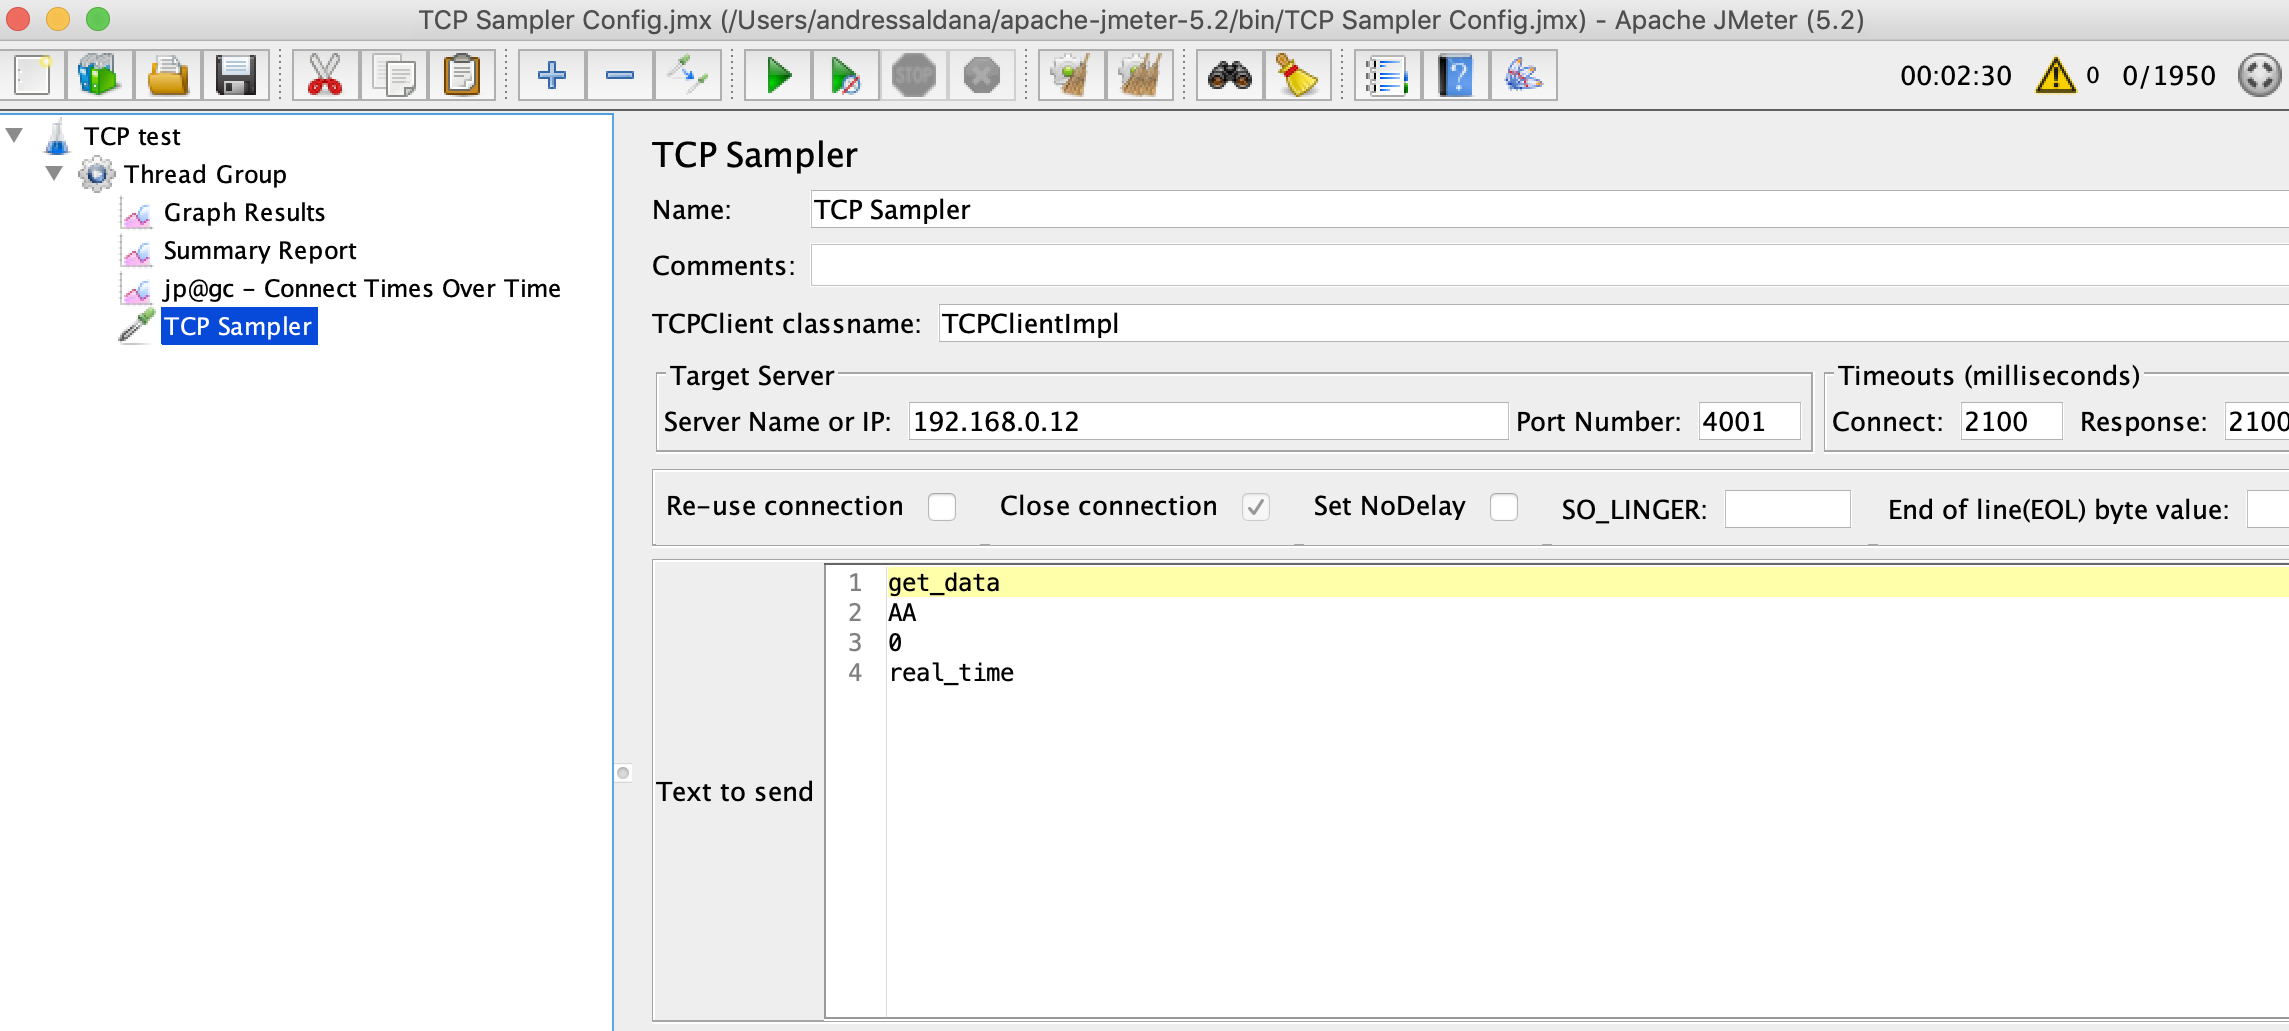
\includegraphics[scale=.3]{Capitulo5/images/real_time_test_config.png}
	\caption{Configuración en JMeter de IP, puerto y mensaje a enviar en texto plano}
	\label{fig:tcpconfig}
\end{figure} 

\begin{figure}[H]
	\centering
	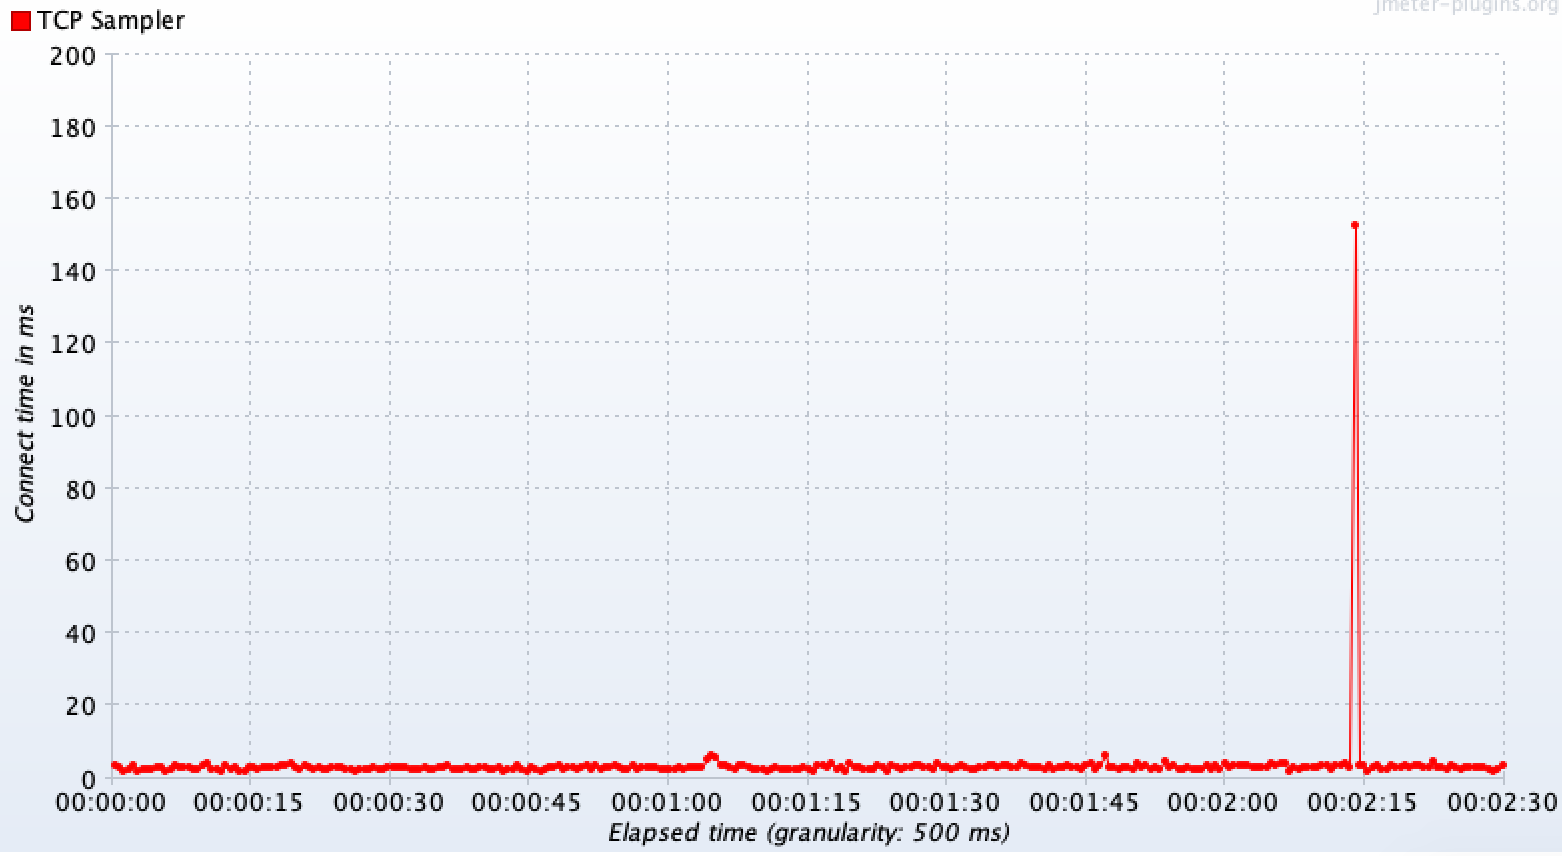
\includegraphics[scale=.3]{Capitulo5/images/real_time_test_connect.png}
	\caption{Gráfica de tiempo de conexión en el tiempo de prueba}
	\label{fig:tcpconnect}
\end{figure} 

\begin{figure}[H]
	\centering
	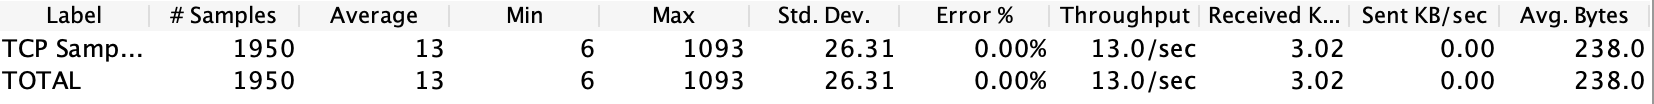
\includegraphics[scale=.5]{Capitulo5/images/real_time_test_summary.png}
	\caption{Resumen de la prueba realizada}
	\label{fig:tcpsummary}
\end{figure} 

\subsection{Integración del modulo del microcontrolador y módulo del servidor embebido}

\subsubsection{Pruebas}
\textbf{Tipo :} Integración \\ \newline

Esta prueba consiste en conocer cuantos nodos provenientes de microcontroladores podemos recibir información y cuántos nodos provenientes de la aplicación se pueden atender de manera simultanea, para ello, creamos una prueba con JMeter que realizara esta simulación en el caso más crítico, guardaremos y accederemos a la información de un mismo nodo \ref{fig:test_integracion}, descubrimos que el máximo de nodos que puede tener la red sin que esta falle \ref{fig:test_integracion_reporte} decrementa y se vuelve constante en 10 nodos y a 10 usuarios accediendo a ellos por segundo, la prueba consto de enviar 1000 a ambos servicios en 100 segundos \ref{fig:test_integracion_config}, sin perder la eficiencia de respuesta del servidor o información, recordando que en TCP JMeter si nos da la cifra real de cuantas peticiones fueron exitosas, pero teniendo que observar el acumulado de producción en el caso de UDP para conocer la tasa de éxito \ref{fig:test_integracion_udp}.

\begin{figure}[H]
	\centering
	\includegraphics[scale=.5]{Capitulo5/images/test_integracion.png}
	\caption{Árbol de la prueba de integración de pruebas unitarias}
	\label{fig:test_integracion}
\end{figure}

\begin{figure}[H]
	\centering
	\includegraphics[scale=.4]{Capitulo5/images/test_integracion_config.png}
	\caption{Configuración de la prueba}
	\label{fig:test_integracion_config}
\end{figure}

\begin{figure}[H]
	\centering
	\includegraphics[scale=.5]{Capitulo5/images/test_integracion_summary.png}
	\caption{Reporte de la prueba de integración}
	\label{fig:test_integracion_reporte}
\end{figure}

\begin{figure}[H]
	\centering
	\includegraphics[scale=.5]{Capitulo5/images/test_integracion_udp.png}
	\caption{Resultado de producción acumulada resultado de peticiones UDP}
	\label{fig:test_integracion_udp}
\end{figure}


%********************************************************%

\section{Módulo del la aplicación de usuario}
\subsection{Objetivo}
%Poner las referencias de los CU de app de usuario
Implementar la funcionalidad descrita en los casos de uso \ref{SUB-U-CU1.1}, \ref{SUB-U-CU1.2}, \ref{SUB-U-CU1.3}, \ref{SUB-U-CU1.4}, \ref{SUB-M-CU1.5}, \ref{SUB-U-CU1.6}, \ref{SUB-U-CU1.7}, \ref{SUB-U-CU1.8}, \ref{SUB-U-CU1.9} que se requieren para cumplir con el diseño realizado en la aplicación móvil. 

\subsection{Calculando periodos para los Históricos}
%Cálculo de periodos en Historical Fragments

\subsubsection{Desarrollo}
Estos procesos están implementados en el lenguaje de programación Java, muy conocido en el ambiente de programación Android, el propósito de este proceso es calcular los periodos de tiempo comprendidos en la pantalla de históricos, mencionados y especificados en la  \ref{RN4}, con esto se abarcan todos los posibles casos de consulta del usuario, es decir, no importa la fecha u hora en que se haga uso de la aplicación, siempre debe de existir una respuesta por parte de la aplicación móvil. \\ \newline
Para el caso del periodo ''Última semana'', se toma en consideración el día en curso y se hace un retroceso de 6 días, por lo que obtendremos como resultado un total de 7 días los cuales comprenderán la última semana, este proceso hace también distinción si se llegara a tratar del caso en el que la última semana comprendida se encuentra entre dos meses. Finalmente obtenemos como resultado las fechas con el formato especificado en la \ref{RN14}, para así poder identificar de todo el conjunto de muestras que se obtiene del archivo ''daily\_production.json'' cuáles son las que serán útiles para la graficación. \\ \newline
En cuanto al periodo ''Mes actual''  la lógica es similar, sin embargo en esta ocasión un proceso distinto hace el calculo del periodo, desde el primer día del mes hasta el día en curso, de igual forma se obtiene una un arreglo de objetos String con el formato especificado en la \ref{RN14}, esto ayuda a identificar las muestras que se desean del archivo ''daily\_production.json'' para su posterior graficación. \\ \newline
Por último, el periodo ''Anual'' requiere un cálculo para conocer los 9 años anteriores al año actual, por lo que de acuerdo a la fecha actual un proceso nuevo calcula los 9 años previos. \\ \newline
\textbf{Nota :} Tanto los periodos, ayer, mensual, bimestral y año, no requieren como tal un cálculo de periodo, sino un acomodo e interpretación de los datos, por lo cual no se listan anteriormente. 

\subsubsection{Pruebas}
\textbf{Tipo :} Integración \\ \newline
Para la realización de las pruebas se ocupó una herramienta llamada JUnit que ofrece Android, la cual está conformada por un conjunto de bibliotecas que permiten la comprobación del buen funcionamiento de una aplicación, se realizaron pruebas de unidad local, las cuales son pruebas que se ejecutan en una máquina virtual Java y con ayuda del método ''assertEquals'' se indicaron las salidas esperadas y la función con parámetros que tomaría el papel de las entradas; si las entradas arrojaban un valor idéntico al de las salidas, entonces se habrá comprobado el buen funcionamiento de las funciones.  \\ \newline

El código utilizado para la prueba del periodo de tiempo ''Última semana'' fue el siguiente:\\ \newline

%va el códgo de semana
\begin{lstlisting}[language= Java, frame=single]

package com.movil.android.solarmonitor;

import android.os.AsyncTask;
import android.util.Log;
import android.view.View;
import android.widget.AdapterView;
import android.widget.ArrayAdapter;

import com.fasterxml.jackson.core.type.TypeReference;
import com.fasterxml.jackson.databind.ObjectMapper;
import com.github.mikephil.charting.data.BarEntry;
import com.movil.android.connectivity.TCPClient;
import com.movil.android.pojos.Microcontroller;
import com.movil.android.pojos.Sample;

import org.junit.Test;
import org.junit.runner.JUnitCore;
import org.junit.runner.Result;
import org.junit.runner.notification.Failure;

import java.text.ParseException;
import java.text.SimpleDateFormat;
import java.util.ArrayList;
import java.util.Calendar;
import java.util.Collection;
import java.util.Date;
import java.util.GregorianCalendar;
import java.util.Iterator;
import java.util.List;
import java.util.TimeZone;

import static org.junit.Assert.*;

/**
* Example local unit test, which will
execute on the development machine (host).
*
* @see <a href="http://d.android.com/tools/testing">
Testing documentation</a>
*/
public class ExampleUnitTest {

   @Test
   public void entriesCorrect() throws ParseException{
       //numero esperado de entries null
       assertEquals("5/Nov/2019",
       ExampleUnitTest.IntervalosDeGeneracion(0));
       System.out.println
       ("Respuesta exitosa! se esperaba un 5/Nov/2019 y se recibió "+
       ExampleUnitTest.IntervalosDeGeneracion(0));
       //numero esperado de entries yesterdar
       assertEquals("6/Nov/2019", 
       ExampleUnitTest.IntervalosDeGeneracion(1));
       System.out.println
       ("Respuesta exitosa! se esperaba un 6/Nov/2019 y se recibió "+
       ExampleUnitTest.IntervalosDeGeneracion(1));
       //numero esperado de entries missing
       assertEquals("7/Nov/2019", 
       ExampleUnitTest.IntervalosDeGeneracion(2));
       System.out.println
       ("Respuesta exitosa! se esperaba un 7/Nov/2019 y se recibió "
       +ExampleUnitTest.IntervalosDeGeneracion(2));
       //numero esperado de entries best
       assertEquals("8/Nov/2019", 
       ExampleUnitTest.IntervalosDeGeneracion(3));
       System.out.println
       ("Respuesta exitosa! se esperaba un 8/Nov/2019 y se recibió "+
       ExampleUnitTest.IntervalosDeGeneracion(3));
       //numero esperado de entries high
       assertEquals("9/Nov/2019", 
       ExampleUnitTest.IntervalosDeGeneracion(4));
       System.out.println("Respuesta exitosa! 
       se esperaba un 9/Nov/2019 y se recibió 
       "+ExampleUnitTest.IntervalosDeGeneracion(4));
       //numero esperado de entries intermediate
       assertEquals("10/Nov/2019", 
       ExampleUnitTest.IntervalosDeGeneracion(5));
       System.out.
       println("Respuesta exitosa! se esperaba un 10/Nov/2019 y se 
       recibió "+ExampleUnitTest.IntervalosDeGeneracion(5));
       //numero esperado de entries low
       assertEquals("11/Nov/2019", 
       ExampleUnitTest.IntervalosDeGeneracion(6));
       System.out.
       println("Respuesta exitosa! Entries Low, 
       se esperaba un 11/Nov/2019 y se recibió 
       "+ExampleUnitTest.IntervalosDeGeneracion(6));
   }

   public static String IntervalosDeGeneracion(int selector){
       SimpleDateFormat sdf = new SimpleDateFormat("dd.MM.yyyy");
       String currentDateandTime = sdf.format(new Date());
       String[] weekdays = new String[7];
       int pos=0;
       //**************
       List<Date> dates = new ArrayList<Date>();
       Calendar calendar = new GregorianCalendar();
       long DAY_IN_MS = 1000 * 60 * 60 * 24;
       Date fin = new Date();//termina el dia de hoy
       Date inicio = new Date(fin.getTime() - (6 * DAY_IN_MS));
       calendar.setTime(inicio);
       while (calendar.getTime().before(new Date())){
           Date result = calendar.getTime();
           dates.add(result);
           calendar.add(Calendar.DATE, 1);
       }
       //**************
       dates.add(fin);
       for (int i = 6; i>-1;i--){

           String dias = currentDateandTime.substring(0,2);
           int dia = Integer.valueOf(dias)-1;
           dia-=i;
           //weekdays[pos]= dia+currentDateandTime.substring(2);
           Date fecha = dates.get(pos);
           String [] meses = {"Ene","Feb","Mar","Abr","May","Jun",
           "Jul","Ago","Sep","Oct","Nov","Dic"};
           //String [] meses = {"01","02","03","04","05","06",
           "07","08","09","10","11","12"};
           weekdays[pos]= fecha.getDate()+"/"+meses[fecha
           .getMonth()]+"/"+(1900+fecha.getYear());
           pos++;
       }


       if(selector==0){
           return weekdays[0];
       }else if(selector==1){
           return weekdays[1];
       }else if(selector==2){
           return weekdays[2];
       }else if(selector==3){
           return weekdays[3];
       }else if(selector==4){
           return weekdays[4];
       }else if(selector==5){
           return weekdays[5];
       }else{
           return weekdays[6];
       }


   }

}


\end{lstlisting}

En la salida podemos observar que los 7 días que se comprenden son los esperados, por lo que la prueba pudo culminar exitosamente y y las salidas coincidieron con lo arrojado por la función programada, cabe resaltar que la prueba se realizó el día 11 de noviembre del año en curso, por lo que los 7 días están comprendidos a partir del día 5 de noviembre hasta el día 11 de noviembre del 2019. \\ \newline

\begin{figure}[H]
	\centering
	\includegraphics[scale=.4]{Capitulo5/images/PruebasSemanalPeriodo.png}
	\caption{Pruebas de periodo semanal}
	\label{fig:Pruebas_de_periodo_semanal}
\end{figure}

\begin{figure}[H]
	\centering
	\includegraphics[scale=.4]{Capitulo5/images/PruebasSemanalPeriodo2.png}
	\caption{Pruebas de periodo semanal 2}
	\label{fig:Pruebas_de_periodo_semanal2}
\end{figure}

El código utilizado para la prueba del periodo de tiempo ''Mes actual'' fue el siguiente:\\ \newline

\begin{lstlisting}[language= Java, frame=single]
package com.movil.android.solarmonitor;

import android.os.AsyncTask;
import android.util.Log;
import android.view.View;
import android.widget.AdapterView;
import android.widget.ArrayAdapter;

import com.fasterxml.jackson.core.type.TypeReference;
import com.fasterxml.jackson.databind.ObjectMapper;
import com.github.mikephil.charting.data.BarEntry;
import com.movil.android.connectivity.TCPClient;
import com.movil.android.pojos.Microcontroller;
import com.movil.android.pojos.Sample;

import org.junit.Test;
import org.junit.runner.JUnitCore;
import org.junit.runner.Result;
import org.junit.runner.notification.Failure;

import java.text.ParseException;
import java.text.SimpleDateFormat;
import java.util.ArrayList;
import java.util.Calendar;
import java.util.Collection;
import java.util.Date;
import java.util.GregorianCalendar;
import java.util.Iterator;
import java.util.List;
import java.util.TimeZone;

import static org.junit.Assert.*;

public class ExampleUnitTest {

   @Test
   public void entriesCorrect() throws ParseException{
       for (int i = 0;i<11;i++){
           //numero esperado de entries null
           assertEquals((i+1)+"/Nov/2019", 
           ExampleUnitTest.IntervalosDeGeneracion(i));
           System.out.println("Respuesta exitosa! 
           Se esperaba un 1/Nov/2019 y se recibió "
           +ExampleUnitTest.IntervalosDeGeneracion(0));

       }
   }

   public static String IntervalosDeGeneracion(int selector){
       SimpleDateFormat formateador = 
       new SimpleDateFormat("MM/dd/yy");
       Date date = new Date();
       String fechaActual = formateador.format(date);
       int numeroMes = Integer.valueOf(fechaActual
       .substring(3,5));
       float a = 8.2f*(((float)numeroMes)/31f);
       int pos=0;
       //**************
       List<Date> dates = new ArrayList<Date>();
       Calendar calendar = new GregorianCalendar();
       long DAY_IN_MS = 1000 * 60 * 60 * 24;
       Date fin = new Date();//termina el dia de hoy
       Date inicio = new Date(fin.getTime() - 
       ((numeroMes-1) * DAY_IN_MS));
       calendar.setTime(inicio);
       while (calendar.getTime().before(new Date())){
           Date result = calendar.getTime();
           dates.add(result);
           calendar.add(Calendar.DATE, 1);
       }
       //**************
       SimpleDateFormat sdf = new SimpleDateFormat("dd.MM.yyyy");
       String currentDateandTime = sdf.format(new Date());
       String[] month = new String[numeroMes];
       String [] meses = {"Ene","Feb","Mar","Abr","May","Jun","Jul"
       ,"Ago","Sep","Oct","Nov","Dic"};
       //String [] meses = {"01","02","03","04","05","06","07","08"
       ,"09","10","11","12"};
       for (int i = numeroMes-2; i>-1;i--){
           String dias = currentDateandTime.substring(0,2);
               /*int dia = Integer.valueOf(dias)-1;
               dia-=i;
               //weekdays[pos]= dia+currentDateandTime.substring(2);*/
           Date fecha = dates.get(pos);
           month[pos]= fecha.getDate()+"/"+meses[fecha.getMonth()]
           +"/"+(1900+fecha.getYear());
           pos++;
       }
       month[numeroMes-1]= fin.getDate()+"/"+meses[fin.getMonth()]
       +"/"+(1900+fin.getYear());
        return month[selector];
   }

}

\end{lstlisting}


Para corroborar que la salida fue la esperada se puso a prueba la función de una manera similar a la del periodo de tiempo ''Última semana'', comparando las salidas con los Strings de fechas correspondientes que comprende el mes actual, al ser consecutivos se puede probar metiendo la función de prueba a un ciclo.

\begin{figure}[H]
	\centering
	\includegraphics[scale=.4]{Capitulo5/images/PruebasMensualPeriodo.png}
	\caption{Pruebas de periodo mensual}
	\label{fig:Pruebas_de_periodo_mensual}
\end{figure}

\begin{figure}[H]
	\centering
	\includegraphics[scale=.4]{Capitulo5/images/PruebasMensualPeriodo2.png}
	\caption{Pruebas de periodo mensual 2}
	\label{fig:Pruebas_de_periodo_mensual2}
\end{figure}

Por último, el código utilizado para la prueba del periodo de tiempo ''Anual'' fue el siguiente:\\ \newline

\begin{lstlisting}[language= Java, frame=single]
package com.movil.android.solarmonitor;

import android.os.AsyncTask;
import android.util.Log;
import android.view.View;
import android.widget.AdapterView;
import android.widget.ArrayAdapter;

import com.fasterxml.jackson.core.type.TypeReference;
import com.fasterxml.jackson.databind.ObjectMapper;
import com.github.mikephil.charting.data.BarEntry;
import com.movil.android.connectivity.TCPClient;
import com.movil.android.pojos.Microcontroller;
import com.movil.android.pojos.Sample;

import org.junit.Test;
import org.junit.runner.JUnitCore;
import org.junit.runner.Result;
import org.junit.runner.notification.Failure;

import java.text.ParseException;
import java.text.SimpleDateFormat;
import java.util.ArrayList;
import java.util.Calendar;
import java.util.Collection;
import java.util.Date;
import java.util.GregorianCalendar;
import java.util.Iterator;
import java.util.List;
import java.util.TimeZone;

import static org.junit.Assert.*;


public class ExampleUnitTest {

   @Test
   public void entriesCorrect() throws ParseException{
       for (int i=0;i<10;i++){
           //numero esperado de entries null
           assertEquals(String.valueOf(2010+i), 
           ExampleUnitTest.IntervalosDeGeneracion(i));
           System.out.println("Respuesta exitosa! se esperaba un "
           +String.valueOf(2010+i)+" y se recibió "+ExampleUnitTest
           .IntervalosDeGeneracion(i));
       }

   }

   public static String IntervalosDeGeneracion(int selector){
       SimpleDateFormat sdf = new SimpleDateFormat("dd.MM.yyyy");
       String currentDateandTime = sdf.format(new Date());
       String actual_Year = currentDateandTime.substring(6);
       String [] years = new String[10];
       for (int i = 9,x=0; i>=0;i--,x++){
           years[i] = String.valueOf(Integer.valueOf(actual_Year)-x);
       }
       return years[selector];
   }

}

\end{lstlisting}

La comprobación para saber si la función está realizando un correcto funcionamiento, es comparar la salida con los 9 años anteriores, ya que serán los valores que deba devolver la función, de ser así la función estaría otorgando salidas acertadas y se comprobará su buen funcionamiento. Al ser de igual forma fechas consecutivas, es posible probar la función dentro de un ciclo. 

\begin{figure}[H]
	\centering
	\includegraphics[scale=.4]{Capitulo5/images/PruebasAnualPeriodo.png}
	\caption{Pruebas de periodo anual}
	\label{fig:Pruebas_de_periodo_anual}
\end{figure}

\begin{figure}[H]
	\centering
	\includegraphics[scale=.4]{Capitulo5/images/PruebasAnualPeriodo2.png}
	\caption{Pruebas de periodo anual 2}
	\label{fig:Pruebas_de_periodo_anual2}
\end{figure}

\subsection{Creando notificaciones y sus distintos tipos}
%Que se cree el objeto Notification para los distintos tipos de notificaciones. LISTO
%Probar todos los tipos de notificaciones hechas al servidor.
%Máximo número de nodos creando hilos que es soportado (Checar si podemos probar creandolos también en la aplicación)%PENDIENTE

%Explicación
Una de las partes fundamentales propuestas en el desarrollo de la aplicación de usuario es la encargada de crear distintos tipos de notificaciones como se ha ido explicación en capítulos anteriores. \\ \newline
Para poder implementar esta funcionalidad en la aplicación, se desarrolló un servicio que estará corriendo en segundo plano para poder realizar una petición cada 10 segundos por cada nodo que existe en el servidor almacenado en el dispositivo móvil, siempre y cuando se cumpla con la regla de negocios \ref{RN18} 
\\ \newline
Si el usuario lo requiere, puede deshabilitar el servicio de monitoreo para notificaciones desactivando el switch de notificaciones en la ventana de 'Configuraciones' de la aplicación móvil.\\ \newline 

\begin{figure}[H]
	\centering
	\includegraphics[scale=.7]{Capitulo5/images/df_notificaciones.png}
	\caption{Diagrama de flujo del servicio de notificaciones}	\label{fig:Diagrama de flujo del servicio de notificaciones}
\end{figure} 

En la figura \ref{fig:Diagrama de flujo del servicio de notificaciones} se muestra un diagrama de flujo que representa la lógica implementada para el servicio de notificaciones que el usuario podrá realizar desde su dispositivo móvil.\\ \newline

\subsubsection{Desarrollo}
Como se puede ver en la figura \ref{fig:Diagrama de flujo del servicio de notificaciones}, se realiza un proceso para identificar sucesos que ameritan crear notificaciones, esto quiere decir, que cuando se crean peticiones al servidor para conocer el valor más actual de las muestras tomadas a los nodos, se interpretará el valor de dicha muestra que es devuelto por el servidor.
\\ \newline
El proceso consiste básicamente en que una vez que la aplicación lanza las peticiones correspondientes al servidor, se esperará una respuesta por parte de él para analizar la muestra y en caso de que no se establezca la conexión con el servidor se dará por hecho que existe una falla.

\subsubsection{Pruebas}
%Especificar tipo de prueba (unitaria, integración, etc.)
\textbf{Tipo :} Unitaria \\ \newline
En esta prueba se parte del hecho de que la aplicación ya lanzó con anterioridad una petición y se recibió una respuesta del servidor, ya sea devolviendo una muestra o que la conexión haya sido rechazada; teniendo esta información y el objeto ''TCPClient'' que se encarga de realizar la petición al servidor se puede identificar el tipo de notificación que se debe de crear.
Para ello los criterios que se toman en cuenta son: si se obtuvo o no respuesta del servidor (falla por conexión) y en caso de que si haya tenido respuesta se lee el valor de la potencia activa (potencia activa de 0 y de -1)
\\ \newline
Para probar que se generan los 3 tipos de notificaciones, se simulan 3 muestras donde cada una de ellas representa un ejemplo en el que se tendría que generar una notificación. Las pruebas invocan al método ''createNotification'' que devolverá un objeto ''Notification'' pasándole como argumento el objeto ''tcpClient'' utilizado para realizar la conexión con el servidor y el objeto ''sample'' que es la simulación de la muestra recibida o no recibida por el servidor, en ese caso será nula. Posteriormente se compara el motivo del objeto ''notification'' que ha sido creado con el que se espera de dicha muestra.  

\begin{lstlisting}[language= Java, frame=single]
package com.movil.android.solarmonitor;

import com.movil.android.connectivity.TCPClient;
import com.movil.android.pojos.Notification;
import com.movil.android.pojos.Sample;

import org.junit.Before;
import org.junit.Test;

import java.text.DateFormat;
import java.text.SimpleDateFormat;
import java.util.Date;

import static org.junit.Assert.assertEquals;

public class NotificationTypesTest {
   TCPClient tcpClientSuccess;// Application server up and running
   TCPClient tcpClientFail;// Application server down
   Sample sampleProduction0;//Sample which active production equals 0
   Sample sampleMissed;//Sample active production equals -1
   Sample sampleNull;//Any sample

   /*Creates a notification in the internal file*/
   public Notification
   createNotification(TCPClient tcpClient, Sample realTimeSample){
       String[] requestInfo = tcpClient.getRequest().split("\n");
       Notification notification = new Notification();
       if(tcpClient.getHasResponse()){
       //0 power production and -1 missing sample notifications
           notification.setActivePower(realTimeSample
           .getActivePower());
           notification.setApparentPower(realTimeSample
           .getApparentPower());
           notification.setCurrent(realTimeSample.getCurrent());
           notification.setDate(realTimeSample.getDate());
           notification.setFrequency(realTimeSample.getFrequency());
           notification.setHour(realTimeSample.getHour());
           notification.setMaxGeneration(realTimeSample
           .getMaxGeneration());
           notification.setMicrocontroller(requestInfo[1]);
           notification.setNode(requestInfo[2]);
           notification.setPowerFactor(realTimeSample
           .getPowerFactor());
           notification.setServer(tcpClient.getServerAddress());
           notification.setVoltage(realTimeSample.getVoltage());
       }
       else{//-2 server not responding notification
           DateFormat sdfDate = new SimpleDateFormat("MM/dd/yy");
           SimpleDateFormat sdfHour = new SimpleDateFormat("HH:mm");
           Date date = new Date();
           notification.setActivePower(-2);
           notification.setApparentPower(0);
           notification.setCurrent(0);
           notification.setDate(sdfDate.format(date));
           notification.setFrequency(0);
           notification.setHour(sdfHour.format(date));
           notification.setMaxGeneration(0);
           notification.setMicrocontroller(requestInfo[1]);
           notification.setNode(requestInfo[2]);
           notification.setPowerFactor(0);//Server error
           notification.setServer(tcpClient.getServerAddress());
           notification.setVoltage(0);
       }
       return notification;
   }

   @Before
   public void init(){
       tcpClientSuccess = new TCPClient(null);
       tcpClientSuccess.setRequest("get_data\nAA\n0\nreal_time");
       tcpClientSuccess.setHasResponse(true);
       tcpClientSuccess.setServerAddress("104.198.212.166");

       tcpClientFail = new TCPClient(null);
       tcpClientFail.setRequest("get_data\nAA\n0\nreal_time");
       tcpClientFail.setHasResponse(false);
       tcpClientFail.setServerAddress("104.198.212.166");

       sampleProduction0 = new Sample();
       sampleProduction0.setActivePower(0);//Criteria
       sampleProduction0.setApparentPower(0);
       sampleProduction0.setCurrent(0);
       sampleProduction0.setDate("11/11/19");
       sampleProduction0.setFrequency(0);
       sampleProduction0.setHour("09:00");
       sampleProduction0.setMaxGeneration(0);
       sampleProduction0.setVoltage(0);

       sampleMissed = new Sample();
       sampleMissed.setActivePower(-1);//Criteria
       sampleMissed.setApparentPower(0);
       sampleMissed.setCurrent(0);
       sampleMissed.setDate("11/11/19");
       sampleMissed.setFrequency(0);
       sampleMissed.setHour("09:00");
       sampleMissed.setMaxGeneration(0);
       sampleMissed.setVoltage(0);

       sampleNull = new Sample();

   }

   @Test
   public void SampleProduction0Test(){
       Notification notification =
       createNotification(tcpClientSuccess, sampleProduction0);
       assertEquals("La notificación fue creada correctamente",
       "Motivo: Potencia Activa= 0",
       notification.showReason());
       System.out.println("La notificación fue creada correctamente: "
       + notification.showReason());
   }

   @Test
   public void SampleMissedTest(){
       Notification notification =  
       createNotification(tcpClientSuccess, sampleMissed);
       assertEquals("La notificación fue creada correctamente",
       "Motivo: Muestra perdida",
       notification.showReason());
       System.out.println("La notificación fue creada correctamente: "
       + notification.showReason());
   }

   @Test
   public void ServerDownTest(){
       Notification notification =  
       createNotification(tcpClientFail, sampleNull);
       assertEquals("La notificación fue creada correctamente",
       "Motivo: Sin respuesta de servidor",
       notification.showReason());
       System.out.println("La notificación fue creada correctamente: "+
       notification.showReason());
   }
}
}
\end{lstlisting}

\begin{figure}[H]
	\centering
	\includegraphics[scale=.7]{Capitulo5/images/pruebaUnitariaNotificaciones.png}
	\caption{Prueba unitaria de creación de notificaciones}	\label{fig:prueba unitaria notificaciones}
\end{figure} 

El resultado de la prueba unitaria se puede observar en la figura \ref{fig:prueba unitaria notificaciones}, en donde indica que se crearon las notificaciones por las causas indicadas de manera exitosa.

\subsubsection{Desarrollo}
Como se menciona en la prueba unitaria anterior, se parte del hecho de que la petición ya fue realizada por la aplicación de usuario; en esta sección se abarcará desde que se crea la petición, se envía al servidor, se recibe la respuesta del servidor y se identifica el tipo de muestra para que posteriormente se pueda analizar si es necesario crear la notificación en la aplicación. 
\\ \newline
Con el objeto de evitarle al usuario recibir una gran cantidad de notificaciones por fallas que pueden persistir durante cierto tiempo, se definió que para las notificaciones por causa de potencia activa igual a 0 o bien de muestra de nodo perdida, se creará únicamente la notificación si se cumple que para ese nodo en particular se vuelva a presentar la falla al menos una hora después del último registro que se tiene almacenado; en el caso de la falla que ocurre por error de conexión con el servidor, se le volverá a hacer una notificación al usuario siempre y cuando se vuelva a presentar al menos 10 minutos después del último registro que se tiene almacenado.

\begin{figure}[H]
	\centering
	\includegraphics[scale=.45]{Capitulo5/images/df_notificacionServidor.png}
	\caption{Diagrama de flujo de peticiones a servidor para notificaciones}	
	\label{fig:Diagrama de flujo de peticiones a servidor para notificaciones}
\end{figure} 

En la figura \ref{fig:Diagrama de flujo de peticiones a servidor para notificaciones} se puede observar el criterio anteriormente explicado para la creación y el almacenamiento de nuevas notificaciones en el dispositivo móvil.

\subsubsection{Pruebas}
\textbf{Tipo :} Integración \\ \newline
Como pruebas de integración, es decir poner a prueba la aplicación móvil haciendo peticiones al servidor, decidimos demostrar como se tiene el servicio activo de notificaciones en el que se lanza peticiones a nuestro servidor y provocamos de lado del servidor que las muestras que se están almacenando sean motivo para que de lado de la aplicación móvil se genere una notificación.
\\ \newline
Teniendo el archivo que almacena las notificaciones vacío, las pruebas se describen a continuación.
\\ \newline
De lado del servidor se detuvo el servicio que se encarga de obtener las muestras del nodo sensor, por lo que al no obtener una lectura almacenará la muestra en el archivo con un valor de -1.

\begin{figure}[H]
	\centering
	\includegraphics[scale=.7]{Capitulo5/images/muestra1.png}
	\caption{Ejemplo de muestra -1 obtenida, se escribe en el archivo}	
	\label{fig:muestra 1}
\end{figure} 

\begin{figure}[H]
	\centering
	\includegraphics[scale=.7]{Capitulo5/images/muestra2.png}
	\caption{Ejemplo de muestra -1 obtenida, no  se escribe en el archivo}	
	\label{fig:muestra 2}
\end{figure} 

\begin{figure}[H]
	\centering
	\includegraphics[scale=.7]{Capitulo5/images/muestra3.png}
	\caption{Se crea la notificación de muestra -1 obtenida}	
	\label{fig:muestra 3}
\end{figure} 

\begin{figure}[H]
	\centering
	\includegraphics[scale=.7]{Capitulo5/images/muestra4.png}
	\caption{Notificación de muestra -1 almacenada}	
	\label{fig:muestra 4}
\end{figure} 

En la figura \ref{fig:muestra 1} se observa que se tiene una lectura de una muestra normal eso se identifica con el mensaje ''realTimeSample Ok'', sin embargo en ese momento detuvimos el servidor de microcontrolador por lo que en la siguiente respuesta de muestra obtuvimos el mensaje ''realTimeSample = -1'' y ''overwriteNotificationFile = true'' lo cual indica que se detectó una muestra perdida y que fue almacenada en el archivo de notificaciones así como se creó una notificación en el dispositivo móvil. 
\\ \newline
En la figura \ref{fig:muestra 2}, como el servicio sigue inactivo se vuelve a detectar una muestra perdida con el mensaje ''realTimeSample = -1'' pero a difierencia de la anterior se observa el mensaje ''overwriteNotificationFile = false'' esto indica que se detectó una muestra perdida pero que no se crea ni se almacena una notificación pues no se ha cumplido con la regla establecida de tiempo de que únicamente se volverá a notificar si la falla ocurré al menos una hora después.
\\ \newline
En la figura \ref{fig:muestra 3} se observa la notificación que fue creada en el dispositivo móvil por la muestra perdida.
\\ \newline
Si ingresamos a la aplicación y nos dirigimos a la lista de notificaciones se observa algo como la figura \ref{fig:muestra 4} que muestra la notificación almacenada. 
\\ \newline

La siguiente prueba que se realizó, se obtuvo deteniendo el servicio que atiende a las peticiones de usuario en el servidor. 

\begin{figure}[H]
	\centering
	\includegraphics[scale=.7]{Capitulo5/images/muestra5.png}
	\caption{Peticiones lanzadas al servidor sin respuesta}	
	\label{fig:muestra 5}
\end{figure} 

\begin{figure}[H]
	\centering
	\includegraphics[scale=.65]{Capitulo5/images/muestra6.png}
	\caption{El servicio está inactivo y se recibe la notificación en el dispositivo}	
	\label{fig:muestra 6}
\end{figure} 

\begin{figure}[H]
	\centering
	\includegraphics[scale=.7]{Capitulo5/images/muestra7.png}
	\caption{Notificación por no tener respuesta del servidor almacenada}	
	\label{fig:muestra 7}
\end{figure} 

\begin{figure}[H]
	\centering
	\includegraphics[scale=.7]{Capitulo5/images/muestra8.png}
	\caption{Notificación por no tener respuesta del servidor que no es almacenada}	
	\label{fig:muestra 8}
\end{figure} 

\begin{figure}[H]
	\centering
	\includegraphics[scale=.6]{Capitulo5/images/muestra9.png}
	\caption{Se crea una nueva notificación por que han pasado 10 minutos}	
	\label{fig:muestra 9}
\end{figure} 

\begin{figure}[H]
	\centering
	\includegraphics[scale=.7]{Capitulo5/images/muestra10.png}
	\caption{Notificaciones por no recibir respuesta del servidor almacenadas}	
	\label{fig:muestra 10}
\end{figure} 

En las figuras \ref{fig:muestra 5} y \ref{fig:muestra 6} se observa como al tener el servicio que atiene a las peticiones de la aplicación inactivo se detecta como una notificación por lo que se crea en el dispositivo y se almacena en el archivo de notificaciones. Esto se identifica por el mensaje ''Error creating socket'' y ''Connection refused''.
\\ \newline
En la figura \ref{fig:muestra 7} se observa la nueva notificación almacenada en el dispositivo.
\\ \newline
En la figura \ref{fig:muestra 8} se observa como aunque se sigan detectando peticiones rechazadas, no se crea ni se almacena una notificación ya que no se ha cumplido con la regla de que deben de pasar al menos 10 minutos para crear una nueva.
\\ \newline
En las figuras \ref{fig:muestra 9} y \ref{fig:muestra 10} se observa como pasados los 10 minutos y con el servicio del servidor que atiende las peticiones del servidor inactivo, se genera una nueva notificación y se almacena en la aplicación.
\\ \newline
%Poner las imagenes para comprobar cuando se detecta un 0
Para poder comprobar el correcto funcionamiento de las notificaciones por generación de energía 0 en un nodo, se procede a editar el archivo ''real\_time.json'', forzándolo a que en el campo de ''Potencia Activa'' el valor sea 0. De esta forma cada que se envíe una petición para conocer el valor de dicha muestra al servidor, se hará lectura de ese campo y se identificará que es candidato a crear una notificación.


\begin{figure}[H]
	\centering
	\includegraphics[scale=.4]{Capitulo4/software/submodulos/images/muestra00.jpg}
	\caption{Se detecta una muestra con producción de energía 0 y se almacena}	
	\label{fig:muestra 11}
\end{figure} 

\begin{figure}[H]
	\centering
	\includegraphics[scale=.4]{Capitulo4/software/submodulos/images/muestra01.jpg}
	\caption{Se detecta otra muestra con producción de energía 0 y no se almacena}	
	\label{fig:muestra 12}
\end{figure} 

\begin{figure}[H]
	\centering
	\includegraphics[scale=.4]{Capitulo4/software/submodulos/images/muestra02.jpg}
	\caption{Notificación creada en el dispositivo}	
	\label{fig:muestra 13}
\end{figure} 

\begin{figure}[H]
	\centering
	\includegraphics[scale=.4]{Capitulo4/software/submodulos/images/muestra03.jpg}
	\caption{Notificación almacenada en el dispositivo}	
	\label{fig:muestra 14}
\end{figure} 

De nuevo, en las figuras \ref{fig:muestra 11} y \ref{fig:muestra 12} se observa como se lanzan un par de peticiones para leer el valor de la muestra más actual del nodo, detecta que el valor de potencia activa es igual a 0 y hace la validación para saber si tiene que crear y almacenar la notificación o si no cumple con la regla establecida de tiempo para volver a crear una nueva notificación.
\\ \newline
En las figuras \ref{fig:muestra 13} y \ref{fig:muestra 14} se observa como se crea la notificación en el dispositivo y se almacena en el archivo de notificaciones.





\subsection{Clasificando muestras de acuerdo al código de colores establecido}
%Clasificación de muestras de acuerdo al código de colores

\subsubsection{Desarrollo}
La clasificación de colores, la cual se encuentra especificada en la \ref{RN12}, ayuda a una mejor visualización de la información de las muestras que se grafica, y gracias a esta clasificación es como el usuario se apoya para poder evaluar el funcionamiento de su sistema fotovoltaico, el correcto funcionamiento de esta función es primordial, ya que en primera instancia es la herramienta de la cual se apoya el usuario tanto para el monitoreo como para la consulta de generación de energía (tanto la generación actual como en los históricos). \\ \newline
La función hace una distinción y a la vez agrupa las muestras en pequeños conjuntos dependiendo sus características, es decir, las muestras que son nulas al conjunto de muestras nulas y así sucesivamente. Además de esto conserva la posición de muestra que es, para que cuando los conjuntos de datos sean mandados a la función que realiza la gráfica, esta pueda saber en qué orden están las muestras a pesar de estar en grupos de muestras diferentes, esto significa que la muestra uno puede encontrarse en un grupo distinto de la muestra dos, pero al momento de ser graficadas estas no pierdan el orden consecutivo.\\ \newline

\subsubsection{Pruebas}
\textbf{Tipo :} Integración \\ \newline
Las pruebas se realizaron proponiendo un arreglo de muestras con los campos de fecha, potencia activa y máxima generación, debido a que estos tres campos son necesarios. El primero de ellos se requiere para uno de los casos en el que la muestra tiene una fecha que no coincide con la del día de hoy, el segundo se requiere para los casos en el que se clasifique de acuerdo a sus porcentajes, a su valor 0 o a su valor de -1, y el tercero de ellos se requiere para poder saber si una muestra está por encima o debajo del 20\% o 50\% de la producción máxima del panel. \\ \newline
El arreglo de muestras es conocido, por lo que se sabe cuántas muestras habrá en cada uno de los conjuntos de muestras al final de ser clasificados, por lo que se hace uso una vez más del método ''assertEquals'' que nos ofrece la herramienta JUnit, y como salida esperada se tendrá el número de muestras que sabemos deberá tener cada conjunto, y como entrada tendrá la función de clasificación, indicado con un entero como parámetro el conjunto de muestras del cual se desea conocer el tamaño una vez terminado el proceso.  \\ \newline
El código que contiene tanto a la función que hace la prueba como a la función a probar es el siguiente: \\ \newline

%Código de clasificación de muestras de acuerdo al código de colores 
\begin{lstlisting}[language= Java, frame=single]
package com.movil.android.solarmonitor;

import android.os.AsyncTask;
import android.util.Log;
import android.view.View;
import android.widget.AdapterView;
import android.widget.ArrayAdapter;

import com.fasterxml.jackson.core.type.TypeReference;
import com.fasterxml.jackson.databind.ObjectMapper;
import com.github.mikephil.charting.data.BarEntry;
import com.movil.android.connectivity.TCPClient;
import com.movil.android.pojos.Microcontroller;
import com.movil.android.pojos.Sample;

import org.junit.Test;
import org.junit.runner.JUnitCore;
import org.junit.runner.Result;
import org.junit.runner.notification.Failure;

import java.text.ParseException;
import java.text.SimpleDateFormat;
import java.util.ArrayList;
import java.util.Calendar;
import java.util.Collection;
import java.util.Date;
import java.util.Iterator;
import java.util.TimeZone;

import static org.junit.Assert.*;

/**
* Example local unit test, which will execute on
the development machine (host).
*
* @see <a href="http://d.android.com/tools/testing">
Testing documentation</a>
*/
public class ExampleUnitTest {

   static ArrayList<BarEntry> entriesNull =
   new ArrayList<BarEntry>();
   static ArrayList<BarEntry> entriesYesterday = 
   new ArrayList<BarEntry>();
   static ArrayList<BarEntry> entriesMissing = 
   new ArrayList<BarEntry>();
   static ArrayList<BarEntry> entriesBest = 
   new ArrayList<BarEntry>();
   static ArrayList<BarEntry> entriesHigh = 
   new ArrayList<BarEntry>();
   static ArrayList<BarEntry> entriesIntermediate = 
   new ArrayList<BarEntry>();
   static ArrayList<BarEntry> entriesLow = 
   new ArrayList<BarEntry>();
   static double bestSample = 170;

   @Test
   public void entriesCorrect() throws ParseException{
       //numero esperado de entries null
       assertEquals(1, ExampleUnitTest.IntervalosDeGeneracion(0));
       System.out.println("Respuesta exitosa! Entries Null,
       se esperaba un 1 y se recibió "
       +ExampleUnitTest.IntervalosDeGeneracion(0));
       //numero esperado de entries yesterdar
       assertEquals(2, ExampleUnitTest.IntervalosDeGeneracion(1));
       System.out.println("Respuesta exitosa! Entries Yesterday,
       se esperaba un 2 y se recibió "
       +ExampleUnitTest.IntervalosDeGeneracion(1));
       //numero esperado de entries missing
       assertEquals(2, ExampleUnitTest.IntervalosDeGeneracion(2));
       System.out.println("Respuesta exitosa! Entries Missing,
       se esperaba un 2 y se recibió "
       +ExampleUnitTest.IntervalosDeGeneracion(2));
       //numero esperado de entries best
       assertEquals(1, ExampleUnitTest.IntervalosDeGeneracion(3));
       System.out.println("Respuesta exitosa! Entries Best,
       se esperaba un 1 y se recibió "
       +ExampleUnitTest.IntervalosDeGeneracion(3));
       //numero esperado de entries high
       assertEquals(3, ExampleUnitTest.IntervalosDeGeneracion(4));
       System.out.println("Respuesta exitosa! Entries High,
       se esperaba un 3 y se recibió "
       +ExampleUnitTest.IntervalosDeGeneracion(4));
       //numero esperado de entries intermediate
       assertEquals(5, ExampleUnitTest.IntervalosDeGeneracion(5));
       System.out.println("Respuesta exitosa! Entries Intermediate,
       se esperaba un 5 y se recibió "
       +ExampleUnitTest.IntervalosDeGeneracion(5));
       //numero esperado de entries low
       assertEquals(6, ExampleUnitTest.IntervalosDeGeneracion(6));
       System.out.println("Respuesta exitosa! Entries Low,
       se esperaba un 6 y se recibió "
       +ExampleUnitTest.IntervalosDeGeneracion(6));
   }

   public static int IntervalosDeGeneracion(int selector)
   throws ParseException {
       entriesNull = new ArrayList<BarEntry>();
       entriesYesterday = new ArrayList<BarEntry>();
       entriesMissing = new ArrayList<BarEntry>();
       entriesBest = new ArrayList<BarEntry>();
       entriesHigh = new ArrayList<BarEntry>();
       entriesIntermediate = new ArrayList<BarEntry>();
       entriesLow = new ArrayList<BarEntry>();

       Sample [] samples = {
               new Sample("11/11/19",15,200),
               new Sample("11/11/19",20,200),
               new Sample("11/11/19",30,200),
               new Sample("11/11/19",70,200),
               new Sample("11/11/19",-1,200),
               new Sample("11/11/19",0,200),
               new Sample("11/10/19",120,200),
               new Sample("11/11/19",150,200),
               new Sample("11/11/19",150,200),
               new Sample("11/11/19",170,200),
               new Sample("11/11/19",150,200),
               new Sample("11/11/19",80,200),
               new Sample("11/11/19",80,200),
               new Sample("11/11/19",10,200),
               new Sample("11/10/19",10,200),
               null,
               new Sample("11/11/19",-1,200),
               new Sample("11/11/19",0,200),
               new Sample("11/11/19",70,200),
               new Sample("11/11/19",70,200)


       };

       SimpleDateFormat sdfDate = new SimpleDateFormat("MM/dd/yy");
       Calendar calendar = Calendar.getInstance();
       TimeZone tz = TimeZone.getDefault();
       calendar.setTimeZone(tz);
       calendar.setTime(new Date());//actual hour and minute


       for(int i = 0; i < samples.length; i++){
           //setting circle colors
           if(samples[i] == null){//firs time 
           initializing, null objects
               entriesNull.add(new BarEntry(i, -1));
           }
           else if(calendar.get(Calendar.DAY_OF_MONTH) != 
           sdfDate.parse(samples[i].getDate()).getDate()){
           //if it is different day (i.e yesterday) 
           The service was turned off
               entriesYesterday.add(new BarEntry(i, -1));
           }
           else if((float)samples[i].getActivePower()
           < 0){//missing samples
               entriesMissing.add(new BarEntry(i, -1));
           }
           /*else if((float)samples[i].getActivePower()
           == 0){//0's samples
               entriesZero.add(new BarEntry(i, 0));
           }*/
           else if((double)samples[i].getActivePower()
           == bestSample){//best samples
               entriesBest.add(new BarEntry(i,
               (float)samples[i].getActivePower()));
           }
           else{//regular samples
               double percentage = 
               (samples[i].getActivePower()*100)/
               samples[i].getMaxGeneration();
               if( percentage >=50 ){
                   entriesHigh.add(new BarEntry(i,
                   (float)samples[i].getActivePower()));
               }
               else if( percentage >= 20 ){
                   entriesIntermediate.add(new BarEntry(i, 
                   (float)samples[i].getActivePower()));
               }
               else{
                   entriesLow.add(new BarEntry(i, 
                   (float)samples[i].getActivePower()));
               }
           }
       }


       if(selector==0){
           return Integer.valueOf(entriesNull.size());
       }else if(selector==1){
           return Integer.valueOf(entriesYesterday.size());
       }else if(selector==2){
           return Integer.valueOf(entriesMissing.size());
       }else if(selector==3){
           return Integer.valueOf(entriesBest.size());
       }else if(selector==4){
           return Integer.valueOf(entriesHigh.size());
       }else if(selector==5){
           return Integer.valueOf(entriesIntermediate.size());
       }else{
           return Integer.valueOf(entriesLow.size());
       }
   }

}

\end{lstlisting}

La salida obtenida nos indica que no hubo ningún inconveniente y que todos los datos esperados coinciden con los obtenidos por la función que se probó, por lo que queda demostrado el correcto funcionamiento a la hora de clasificar las muestras. 

%Capturas de pantalla de salida en consola 
\begin{figure}[H]
	\centering
	\includegraphics[scale=.4]{Capitulo5/images/PruebaCodigoDeColores.png}
	\caption{Respuesta a la prueba de la función de clasificación de código de colores}	
	\label{fig:Codigo_de_colores}
\end{figure} 

\begin{figure}[H]
	\centering
	\includegraphics[scale=.4]{Capitulo5/images/PruebaCodigoDeColores2.png}
	\caption{Respuesta a la prueba de la función de clasificación de código de colores 2}	
	\label{fig:Codigo_de_colores2}
\end{figure} 

\subsection{Clasificando muestras de acuerdo al valor de máxima generación del panel}

\subsubsection{Desarrollo}
Al ser una de las funciones más utilizadas, a pesar de estar considerada en la clasificación anterior, el porcentaje mayor de las muestras recae en esta función, y requieren ser clasificadas dependiendo de si son menor al 20\% de la producción máxima del panel, si se encuentran en el rango entre el 20\% y el 50\%, o si están por encima del 50\% de la producción máxima del panel. \\ \newline

\subsubsection{Pruebas}
\textbf{Tipo :} Integración \\ \newline
Una vez más partiendo de un arreglo conocido de muestras con los parámetros de fecha, potencia activa y máxima generación del panel, se calculan los porcentajes de acuerdo al último parámetro mencionado y se clasifican dentro de 3 conjuntos de muestras, dependiendo de el rango en el que se encuentren. Cae mencionar que para poder ser clasificadas las muestras de esta manera, tienen antes que haber sido evaluadas y descartar que sean muestras antiguas con generación 0, con generación -1 o ser una muestra nula. \\ \newline

El código utilizado para generar las pruebas de dicha función es el siguiente, utilizando el método ''assertEquals'' de la herramienta JUnit:\\ \newline
%Código de Clasificación de muestras por intervalo de max generación
\begin{lstlisting}[language= Java, frame=single]
package com.movil.android.solarmonitor;

import android.os.AsyncTask;
import android.util.Log;
import android.view.View;
import android.widget.AdapterView;
import android.widget.ArrayAdapter;

import com.fasterxml.jackson.core.type.TypeReference;
import com.fasterxml.jackson.databind.ObjectMapper;
import com.github.mikephil.charting.data.BarEntry;
import com.movil.android.connectivity.TCPClient;
import com.movil.android.pojos.Microcontroller;
import com.movil.android.pojos.Sample;

import org.junit.Test;
import org.junit.runner.JUnitCore;
import org.junit.runner.Result;
import org.junit.runner.notification.Failure;

import java.text.ParseException;
import java.text.SimpleDateFormat;
import java.util.ArrayList;
import java.util.Calendar;
import java.util.Collection;
import java.util.Date;
import java.util.Iterator;
import java.util.TimeZone;

import static org.junit.Assert.*;

/**
* Example local unit test, which will execute on
the development machine (host).
*
* @see <a href="http://d.android.com/tools/testing">
Testing documentation</a>
*/
public class ExampleUnitTest {

   static ArrayList<BarEntry> entriesNull = new ArrayList<BarEntry>();
   static ArrayList<BarEntry> entriesYesterday = 
   new ArrayList<BarEntry>();
   static ArrayList<BarEntry> entriesMissing = 
   new ArrayList<BarEntry>();
   static ArrayList<BarEntry> entriesBest = 
   new ArrayList<BarEntry>();
   static ArrayList<BarEntry> entriesHigh = 
   new ArrayList<BarEntry>();
   static ArrayList<BarEntry> entriesIntermediate =
   new ArrayList<BarEntry>();
   static ArrayList<BarEntry> entriesLow = 
   new ArrayList<BarEntry>();
   static double bestSample = 170;

   @Test
   public void entriesCorrect() throws ParseException{
       //numero esperado de entries high
       assertEquals(5, ExampleUnitTest.IntervalosDeGeneracion(0));
       System.out.println("Respuesta exitosa! Entries High,
       se esperaba un 5 y se recibió
       "+ExampleUnitTest.IntervalosDeGeneracion(0));
       //numero esperado de entries intermediate
       assertEquals(5, ExampleUnitTest.IntervalosDeGeneracion(1));
       System.out.println("Respuesta exitosa! Entries Intermediate,
       se esperaba un 5 y se recibió 
       "+ExampleUnitTest.IntervalosDeGeneracion(1));
       //numero esperado de entries low
       assertEquals(10, ExampleUnitTest.IntervalosDeGeneracion(2));
       System.out.println("Respuesta exitosa! Entries Low,
       se esperaba un 10 y se recibió 
       "+ExampleUnitTest.IntervalosDeGeneracion(2));
   }

   public static int IntervalosDeGeneracion(int selector)
   throws ParseException {
       entriesNull = new ArrayList<BarEntry>();
       entriesYesterday = new ArrayList<BarEntry>();
       entriesMissing = new ArrayList<BarEntry>();
       entriesBest = new ArrayList<BarEntry>();
       entriesHigh = new ArrayList<BarEntry>();
       entriesIntermediate = new ArrayList<BarEntry>();
       entriesLow = new ArrayList<BarEntry>();

       Sample [] samples = {
               new Sample("11/11/19",15,200),
               new Sample("11/11/19",20,200),
               new Sample("11/11/19",30,200),
               new Sample("11/11/19",70,200),
               new Sample("11/11/19",25,200),
               new Sample("11/11/19",15,200),
               new Sample("11/11/19",120,200),
               new Sample("11/11/19",150,200),
               new Sample("11/11/19",150,200),
               new Sample("11/11/19",170,200),
               new Sample("11/11/19",150,200),
               new Sample("11/11/19",80,200),
               new Sample("11/11/19",80,200),
               new Sample("11/11/19",10,200),
               new Sample("11/11/19",10,200),
               new Sample("11/11/19",20,200),
               new Sample("11/11/19",11,200),
               new Sample("11/11/19",70,200),
               new Sample("11/11/19",14,200),
               new Sample("11/11/19",70,200)


       };

       SimpleDateFormat sdfDate = new SimpleDateFormat("MM/dd/yy");
       Calendar calendar = Calendar.getInstance();
       TimeZone tz = TimeZone.getDefault();
       calendar.setTimeZone(tz);
       calendar.setTime(new Date());//actual hour and minute


       for(int i = 0; i < samples.length; i++){
           //regular samples
           double percentage = (samples[i].getActivePower()*100)
           /samples[i].getMaxGeneration();
           if( percentage >=50 ){
               entriesHigh.add(new BarEntry(i, 
               (float)samples[i].getActivePower()));
           }
           else if( percentage >= 20 ){
               entriesIntermediate.add(new BarEntry(i,
               (float)samples[i].getActivePower()));
           }
           else{
               entriesLow.add(new BarEntry(i, 
               (float)samples[i].getActivePower()));
           }

       }

       System.out.println(entriesHigh.size()+" 
       "+entriesIntermediate.size()+" "+entriesLow.size());

       if(selector==0){
           return Integer.valueOf(entriesHigh.size());
       }else if(selector==1){
           return Integer.valueOf(entriesIntermediate.size());
       }else{
           return Integer.valueOf(entriesLow.size());
       }
   }

}

\end{lstlisting}

Al ser un arreglo de muestras conocido, se comparan las salidas esperadas con las salidas de la función, así comprobando el contenido de cada uno de los conjuntos en los que fueron clasificadas las muestras y verificando que las salidas sean acertadas. 

\begin{figure}[H]
	\centering
	\includegraphics[scale=.4]{Capitulo5/images/PruebaMaxGeneracion.png}
	\caption{Respuesta a la prueba de la función de clasificación por máxima generación}	
	\label{fig:Codigo_de_colores}
\end{figure} 

\begin{figure}[H]
	\centering
	\includegraphics[scale=.4]{Capitulo5/images/PruebaMaxGeneracion2.png}
	\caption{Respuesta a la prueba de la función de clasificación por máxima generación 2}	
	\label{fig:Codigo_de_colores}
\end{figure} 



\subsection{Graficando  muestras (Generación Actual e Históricos)}
\subsubsection{Desarrollo}
La graficación es la esencia de la aplicación de usuario, puesto que en ella se basa y fundamenta todo lo que el sistema tiene para mostrar al usuario, sin embargo resulta una tarea que es complementada por muchos procesos que hacen posible que las gráficas aparezcan en la pantalla del dispositivo móvil. \\ \newline
Existen diferentes tipos de peticiones, así como casos en los cuales se usarán, sin embargo para los casos específicos de graficación, la petición siempre deberá de ser declarada de la siguiente forma: \\ \newline
\newline
\textbf{get\_data} \newline
\textbf{microcontrolador\_seleccionado} \newline
\textbf{nodo\_seleccionado} \newline
\textbf{archivo\_seleccionado} \newline
\newline
\textbf{Ejemplo:} \newline
\newline
\textbf{get\_data} \newline
\textbf{AA} \newline
\textbf{0} \newline
\textbf{yesterday\_samples} \newline
\newline
Los valores deberán estar separados por saltos de línea, esto para que el servidor pueda descomponer la petición e identificar los elementos que están inmersos en ella. Las únicas dos secciones que pueden y deben hacer uso de esta petición, son la sección de producción actual y la de históricos dentro de la aplicación. El diagrama de flujo que explica el proceso de obtención de muestras se especifica en la figura \ref{fig:Diagrama de flujo para graficar} \\ \newline

\begin{figure}[H]
	\centering
	\includegraphics[scale=.6]{Capitulo5/images/DiagramaDeFlujoGraficar.JPG}
	\caption{Diagrama de flujo para graficar}	\label{fig:Diagrama de flujo para graficar}
\end{figure} 

La clase principal y la que se encarga de la comunicación con el servidor, es la clase ConnectTask, la cual se especifica a detalle en la siguiente sección ''Obteniendo muestras provenientes del servidor dada una petición''. \\ \newline

Una vez recibidas las muestras se procede a clasificarlas para así poder graficarlas con un formato de colores que permita la fácil identificación y entendimiento de los datos, esta clasificación está especificada en la \ref{RN12} y es un proceso por el cual se debe pasar obligatoriamente antes de poder graficar las muestras. \\ \newline
Finalmente las muestras son graficadas, en el caso de la producción actual el gráfico no es necesario que modifique sus características o parámetros, puesto que lo único que se actualiza son las muestras, sin embargo, en el caso de los históricos, tanto el numero de muestras como los mismos datos y archivos que se consultan, varían dependiendo del periodo de tiempo que se seleccione, quedando clasificados de la siguiente manera el archivo que es consultado y los periodos que lo consultan: \\ \newline
\newline
\textbf{Archivo yesterday\_samples.json: }periodo Ayer \newline
\textbf{Archivo daily\_production.json: }periodos Última semana y Mes actual \newline
\textbf{Archivo monthly\_production.json: }periodos Mensual y Bimestral \newline
\textbf{Archivo yearly\_production.json: }periodos Última década y Año \newline
\newline
El periodo de Ayer es el único que va a hacer uso del código de colores puesto que al ser muestras y no acumulados de muestras, pueden evaluarse, sin embargo las demás gráficas al ser un acumulado de muestras durante el periodo que indique su archivo (daily\_production, monthly\_production o) se graficarán todas de un color uniforme, exceptuando la muestra mayor, la cual seguirá destacando con un color distinto. \\ \newline
Otra modificación que sufren las gráficas de históricos, son tanto la posibilidad de hacer un acercamiento a las barras de la gráfica (zoom), como los valores que toma el eje X, ya que se trata de periodos de tiempo distintos, por ello se hace un cálculo de periodo de históricos el cuál se especificó previamente.

\subsubsection{Pruebas}
\textbf{Tipo: }Unitaria \newline
Las pruebas de este módulo están enfocadas al tiempo de respuesta y esta primera prueba específicamente al tiempo de graficación, es decir, partiendo desde el punto en que el servidor ha dado respuesta a la petición de la aplicación de usuario con el archivo que contiene las muestras correspondientes, hasta el instante en que es capaz la aplicación de usuario de hacer el renderizado de la gráfica y logra mostrar las muestras clasificadas, en orden y en los tiempos que se establecieron en los requerimientos no funcionales. \\ \newline
Se agregaron las siguientes lineas de código en la clase encargada de la graficación de generación actual para tener un control del inicio y el fin del proceso, la figura \ref{fig:Tiempo_Graficacion} toma la muestra de tiempo del sistema en el instante en que se comienza la graficación, mientras que la \ref{fig:Tiempo_Graficacion2} toma de igual forma la muestra de tiempo del sistema, pero en el momento en que termina la graficación, entonces resta el tiempo final menos el inicial y obtiene el tiempo total de graficación. \\ \newline

%tiempo de graficacion imagenes CODIGO
\begin{figure}[H]
	\centering
	\includegraphics[scale=.6]{Capitulo5/images/TiempoGraficacionCodigo.png}
	\caption{Fragmento de código que inicia el conteo del tiempo en la grafica de generación actual.}	\label{fig:Tiempo_Graficacion}
\end{figure} 

\begin{figure}[H]
	\centering
	\includegraphics[scale=.6]{Capitulo5/images/TiempoGraficacionCodigo2.png}
	\caption{Fragmento de código que termina el conteo y obtiene el tiempo total en la grafica de generación actual.}	\label{fig:Tiempo_Graficacion2}
\end{figure} 

Los resultados se ven reflejados en las salidas a consola de la aplicación, en donde podemos observar que los tiempos son adecuados a los estándares establecidos en los requerimientos no funcionales y quedando un buen tiempo de holgura.  \\ \newline

\begin{figure}[H]
	\centering
	\includegraphics[scale=.6]{Capitulo5/images/TiempoGraficacionGAResultado.png}
	\caption{Resultado que muestra tanto la marca de tiempo de inicio como el tiempo que tardó en mostrar la grafica de Generacion Actual}	\label{fig:Tiempo_GraficacionGAR}
\end{figure} 

En cuanto a la clase encargada de la graficación de históricos, se siguió un proceso similar, en donde en la figura \ref{fig:Tiempo_GraficacionH} se colocó el código que da inicio al contador y en los fragmentos que correspondían a cada uno de los periodos de tiempo se colocó el código que daría tiempo a ese contador, como se especifica en la figura \ref{fig:Tiempo_GraficacionH2}. \\ \newline

\begin{figure}[H]
	\centering
	\includegraphics[scale=.6]{Capitulo5/images/TiempoGraficacionHistCodigo.png}
	\caption{Fragmento de código que inicia el conteo del tiempo en la grafica de históricos.}	\label{fig:Tiempo_GraficacionH}
\end{figure} 

\begin{figure}[H]
	\centering
	\includegraphics[scale=.5]{Capitulo5/images/TiempoGraficacionHistCodigo2.png}
	\caption{Fragmentos de código que terminan el conteo y obtienen el tiempo total en la grafica de históricos.}	\label{fig:Tiempo_GraficacionH2}
\end{figure} 

Los resultados son distintos para cada uno de los periodos que abarca la aplicación, dichos resultados siguen cumpliendo con lo establecido en los requerimientos no funcionales.\\ \newline

\begin{figure}[H]
	\centering
	\includegraphics[scale=.6]{Capitulo5/images/TiempoGraficacionAyer.png}
	\caption{Resultados de tiempo de la graficación del periodo histórico ''Ayer''}	\label{fig:Tiempo_GraficacionHAyer}
\end{figure} 
\begin{figure}[H]
	\centering
	\includegraphics[scale=.6]{Capitulo5/images/TiempoGraficacionUltimaSemana.png}
	\caption{Resultados de tiempo de la graficación del periodo histórico ''Última Semana''}	\label{fig:Tiempo_GraficacionHUltimaSemana}
\end{figure} 
\begin{figure}[H]
	\centering
	\includegraphics[scale=.6]{Capitulo5/images/TiempoGraficacionMesActual.png}
	\caption{Resultados de tiempo de la graficación del periodo histórico ''Mes Actual''}	\label{fig:Tiempo_GraficacionHMesActual}
\end{figure} 
\begin{figure}[H]
	\centering
	\includegraphics[scale=.6]{Capitulo5/images/TiempoGraficacionMensual.png}
	\caption{Resultados de tiempo de la graficación del periodo histórico ''Mensual''}	\label{fig:Tiempo_GraficacionHMensual}
\end{figure} 
\begin{figure}[H]
	\centering
	\includegraphics[scale=.6]{Capitulo5/images/TiempoGraficacionBimestral.png}
	\caption{Resultados de tiempo de la graficación del periodo histórico ''Bimestral''}	\label{fig:Tiempo_GraficacionHBimestral}
\end{figure} 
\begin{figure}[H]
	\centering
	\includegraphics[scale=.6]{Capitulo5/images/TiempoGraficacionUltimaDecada.png}
	\caption{Resultados de tiempo de la graficación del periodo histórico ''Última Decada''}	\label{fig:Tiempo_GraficacionHUltimaDecada}
\end{figure} 
\begin{figure}[H]
	\centering
	\includegraphics[scale=.6]{Capitulo5/images/TiempoGraficacionAno.png}
	\caption{Resultados de tiempo de la graficación del periodo histórico ''Año''}	\label{fig:Tiempo_GraficacionHAno}
\end{figure} 


\textbf{Tipo: }De sistema \newline
El segundo tipo de prueba es el de el tiempo de respuesta, pero ahora incluyendo también el proceso mediante el cual se realiza la petición al servidor y el servidor responde con las muestras solicitadas, es decir, el proceso completo desde que el usuario desea conocer ya sea la producción actual o de algún histórico, hasta el momento en que es mostrada la gráfica en la pantalla del dispositivo del usuario. \\ \newline
Para el caso de la clase encargada de mostrar la grafica de generación actual, se adjuntó como se muestra en la figura \ref{fig:TiempoCompletoGAInicio} la linea de código que inicia el conteo y como se muestra en la figura \ref{fig:TiempoCompletoGAFin}, se adjuntó la linea de código que detiene el conteo y arroja el resultado en milisegundos.\\ \newline

\begin{figure}[H]
	\centering
	\includegraphics[scale=.6]{Capitulo5/images/TiempoCompletoCodigoInicio.png}
	\caption{Código que da inicio al conteo de tiempo en la clase que se encarga de mostrar la gráfica de generación actual.}	\label{fig:TiempoCompletoGAInicio}
\end{figure} 

\begin{figure}[H]
	\centering
	\includegraphics[scale=.5]{Capitulo5/images/TiempoCompletoCodigoFin.png}
	\caption{Código que da fin al conteo de tiempo en la clase que se encarga de mostrar la gráfica de generación actual.}	\label{fig:TiempoCompletoGAFin}
\end{figure} 

Como puede verse en la figura \ref{fig:TiempoCompletoGAResultado}, el tiempo medido es mostrado en consola y se observa que el tiempo es adecuado, coinciden con lo especificado en los requerimientos no funcionales y quedando un tiempo de holgura.\\ \newline

\begin{figure}[H]
	\centering
	\includegraphics[scale=.6]{Capitulo5/images/TiempoCompletoPruebasGA.png}
	\caption{Resultado de la medición de tiempo de la gráfica encargada de mostrar la generación actual.}	\label{fig:TiempoCompletoGAResultado}
\end{figure} 

Siguiendo la misma estructura de mostrar el código de inicio y de fin, a continuación veremos en las figuras \ref{fig:TiempoCompletoHInicio}, \ref{fig:TiempoCompletoHInicio2} y \ref{fig:TiempoCompletoHFin} los dos códigos que pueden dar inicio y fin al conteo de tiempo respectivamente. Existe la posibilidad de tener dos códigos de inicio ya que la petición puede lanzarse al elegir un nuevo nodo o un nuevo periodo de tiempo. \\ \newline

\begin{figure}[H]
	\centering
	\includegraphics[scale=.6]{Capitulo5/images/TiempoCompletoCodigoInicioH.png}
	\caption{Código que da inicio al conteo de tiempo en la clase que se encarga de mostrar las gráficas de históricos en el selector de periodo de tiempo.}	\label{fig:TiempoCompletoHInicio}
\end{figure} 

\begin{figure}[H]
	\centering
	\includegraphics[scale=.6]{Capitulo5/images/TiempoCompletoCodigoInicioH2.png}
	\caption{Código que da inicio al conteo de tiempo en la clase que se encarga de mostrar las gráficas de históricos en el selector de periodo de tiempo.}	\label{fig:TiempoCompletoHInicio2}
\end{figure} 

\begin{figure}[H]
	\centering
	\includegraphics[scale=.5]{Capitulo5/images/TiempoCompletoCodigoFinH.png}
	\caption{Código que da fin al conteo de tiempo en la clase que se encarga de mostrar la gráfica de históricos.}	\label{fig:TiempoCompletoHFin}
\end{figure} 

Los resultados de tiempo obtenidos son mostrados en consola como los anteriores y se puede ver que el tiempo es adecuado, coinciden con lo especificado en los requerimientos no funcionales y quedando un tiempo de holgura de igual forma.\\ \newline

\begin{figure}[H]
	\centering
	\includegraphics[scale=.6]{Capitulo5/images/TiempoCompletoAyer.png}
	\caption{Resultados (tiempo de inicio) de tiempo del proceso completo de graficación y petición del periodo histórico ''Ayer''}	\label{fig:TiempoCompletoHAyer}
\end{figure} 
\begin{figure}[H]
	\centering
	\includegraphics[scale=.6]{Capitulo5/images/TiempoCompletoAyer2.png}
	\caption{Resultados (tiempo total) de tiempo del proceso completo de graficación y petición del periodo histórico ''Ayer''}	\label{fig:TiempoCompletoHAyer2}
\end{figure} 
\begin{figure}[H]
	\centering
	\includegraphics[scale=.6]{Capitulo5/images/TiempoCompletoUltimaSemana.png}
	\caption{Resultados (tiempo de inicio) de tiempo del proceso completo de graficación y petición del periodo histórico ''Ultima Semana''}	\label{fig:TiempoCompletoHUltimaSemana}
\end{figure} 
\begin{figure}[H]
	\centering
	\includegraphics[scale=.6]{Capitulo5/images/TiempoCompletoUltimaSemana2.png}
	\caption{Resultados (tiempo total) de tiempo del proceso completo de graficación y petición del periodo histórico ''Ultima Semana''}	\label{fig:TiempoCompletoHUltimaSemana2}
\end{figure} 
\begin{figure}[H]
	\centering
	\includegraphics[scale=.6]{Capitulo5/images/TiempoCompletoMesActual.png}
	\caption{Resultados (tiempo de inicio) de tiempo del proceso completo de graficación y petición del periodo histórico ''Mes Actual''}	\label{fig:TiempoCompletoHMesActual}
\end{figure} 
\begin{figure}[H]
	\centering
	\includegraphics[scale=.6]{Capitulo5/images/TiempoCompletoMesActual2.png}
	\caption{Resultados (tiempo total) de tiempo del proceso completo de graficación y petición del periodo histórico ''Mes Actual''}	\label{fig:TiempoCompletoHMesActual2}
\end{figure} 
\begin{figure}[H]
	\centering
	\includegraphics[scale=.6]{Capitulo5/images/TiempoCompletoMensual.png}
	\caption{Resultados (tiempo de inicio) de tiempo del proceso completo de graficación y petición del periodo histórico ''Mensual''}	\label{fig:TiempoCompletoHMensual}
\end{figure} 
\begin{figure}[H]
	\centering
	\includegraphics[scale=.6]{Capitulo5/images/TiempoCompletoMensual2.png}
	\caption{Resultados (tiempo total) de tiempo del proceso completo de graficación y petición del periodo histórico ''Mensual''}	\label{fig:TiempoCompletoHMensual2}
\end{figure} 
\begin{figure}[H]
	\centering
	\includegraphics[scale=.6]{Capitulo5/images/TiempoCompletoBimestral.png}
	\caption{Resultados (tiempo de inicio) de tiempo del proceso completo de graficación y petición del periodo histórico ''Bimestral''}	\label{fig:TiempoCompletoHBimestral}
\end{figure} 
\begin{figure}[H]
	\centering
	\includegraphics[scale=.6]{Capitulo5/images/TiempoCompletoBimestral2.png}
	\caption{Resultados (tiempo total) de tiempo del proceso completo de graficación y petición del periodo histórico ''Bimestral''}	\label{fig:TiempoCompletoHBimestral2}
\end{figure} 
\begin{figure}[H]
	\centering
	\includegraphics[scale=.6]{Capitulo5/images/TiempoCompletoUltimaDecada.png}
	\caption{Resultados (tiempo de inicio) de tiempo del proceso completo de graficación y petición del periodo histórico ''Última Decada''}	\label{fig:TiempoCompletoHUltimaDecada}
\end{figure} 
\begin{figure}[H]
	\centering
	\includegraphics[scale=.6]{Capitulo5/images/TiempoCompletoUltimaDecada2.png}
	\caption{Resultados (tiempo total) de tiempo del proceso completo de graficación y petición del periodo histórico ''Última Decada''}	\label{fig:TiempoCompletoHUltimaDecada}
\end{figure} 
\begin{figure}[H]
	\centering
	\includegraphics[scale=.6]{Capitulo5/images/TiempoCompletoAno.png}
	\caption{Resultados (tiempo de inicio) de tiempo del proceso completo de graficación y petición del periodo histórico ''Año''}	\label{fig:TiempoCompletoHAno}
\end{figure} 
\begin{figure}[H]
	\centering
	\includegraphics[scale=.6]{Capitulo5/images/TiempoCompletoAno2.png}
	\caption{Resultados (tiempo total) de tiempo del proceso completo de graficación y petición del periodo histórico ''Año''}	\label{fig:TiempoCompletoHAno}
\end{figure} 




\subsection{Obteniendo muestras provenientes del servidor dada una petición}
%De TCPClient checar que dado un request específico se obtenga el response del servidor
\subsubsection{Desarrollo}
%Explicación
Dentro de las clases desarrolladas en Java para el proyecto de la aplicación en Android más importantes se encuentran ''ConnectTask'' y ''TCPClient''; su importancia radica en que serán utilizadas como base para poder realizar todas las peticiones que el usuario puede hacer mediante la aplicación móvil.
\\ \newline
A grandes rasgos ''TCPClient'' sirve para configurar la dirección IP a la que se enviará la petición, el puerto que el servidor tiene abierto para recibir las peticiones, la petición creada por el cliente (tipo String), y el almacenamiento de la respuesta del servidor en un String o en un archivo temporal dependiendo el tipo de petición. Además en esta clase se define el método ''run()'' el cual se encarga de crear el socket para hacer la conexión con el servidor y se mantiene en un ciclo durante el periodo de escucha de respuesta del servidor, dependiendo del tipo de petición se define si la respuesta se va almacenando en un archcivo temporal o bien en un String, esto se definió debido a que para propósito de hacer la parte de configuración del servidor para almacenarlo en la aplicación móvil basta con recibir la respuesta en un String, mientras que para las peticiones realizadas para la creación de gráficas, al contener mayor información que será analizada posteriormente se almacena en un archivo temporal.
\\ \newline
%Poner referencia de la documentaciòn de Android
La clase de ''ConnectTask'' es realmente una clase interna que ocupa cada uno de los fragments (pantallas) de la aplicación móvil. Esta clase extiende de AsyncTask, la cual es una clase que pertenece a Android y facilita el uso del hilo principal que pertenece a la interfaz de usuario, de tal forma que se pueden realizar operaciones en un hilo secundario y reflejar los resultados en pantalla sin generar conflictos sobre el hilo principal.
\\ \newline
El proceso que se tiene para todas las peticiones que crea la aplicación hacia el servidor, se tiene que crear una instancia de la clase ''ConnectTask'' e invocar al método ''execute()'', el cual recibe como parámetro un arreglo de Strings; este arreglo tiene 2 Strings, el primer valor indica la IP del servidor al cual se le hará la petición y el segundo valor contiene el String formado para cada caso particular de la petición que está por realizarse. Por ejemplo: Si se quiere hacer una petición al servidor con IP 104.198.212.166 para obtener la información del archivo real\_time.json del nodo 0 que pertenece al microcontrolador AA, se crea la siguiente cadena: ''get\_data\\nAA\\n0\\nreal\_time'', primero se especifica el tipo de petición, microcontrolador, nodo y nombre del archivo a consultar, todos separados por un salto de línea representado por ''\\n''.
\\ \newline
Cuando se invoca al método ''execute()'' internamente se le pasa como parámetro a un método que se sobreescribe en el AsyncTask llamado ''doInBackground()'', este método recibe el arreglo de Strings que especificamos en el método ''execute()'' y se realiza la lógica que queremos hacer en el hilo secundario, en nuestro caso implementamos el código que se encarga de hacer la configuración en el objeto de ''TCPClient'' y se invoca al método ''run()'' mencionado anteriormente, es decir, ocupamos el AsyncTask para realizar la conexión con el servidor por medio de un socket TCP en un hilo secundario y una vez que se concluye con este método, se invoca al método ''onPostExecute()'', este método igualmente pertenece al AsyncTask y es invocado una vez que se finaliza la ejecucción definida en ''doInBackground()'', en nuestro caso, se invoca una vez que se ha finalizado la conexión con el servidor. En ''onPostExecute()'' se realizan diferentes tipos de acciones para cada una de las peticiones definidas en la aplicación. Por ejemplo si la petición se realizó para generar la gráfica de hoy, se lee el archivo que contiene la información recibida del servidor, se clasifica para generar el gráfico con su respectivo código de colores y finalmente se muestra la gráfica en pantalla.

\begin{figure}[H]
	\centering
	\includegraphics[scale=.6]{Capitulo5/images/df_connecttask.png}
	\caption{Diagrama de flujo de ConnectTask}
	\label{fig:Diagrama de flujo de ConnectTask}
\end{figure} 

En la figura \ref{fig:Diagrama de flujo de ConnectTask} se muestra un diagrama de flujo que resume la explicación anterior. Como se menciona al inicio, dependiendo de la petición que realiza el usuario es el uso que se le dará a la información recibida del servidor, ya sea leyendo un archivo temporal o un String.

\subsubsection{Pruebas}
\textbf{Tipo: }Integración \newline
Para probar el funcionamiento de ConnectTask, se mostrarán algunas capturas de pantalla que muestran diferentes casos en los que el usuario realiza una acción en la aplicación móvil que detona una petición.  
\\ \newline
La parte importante que se debe detectar de cada una de las imágenes que se están por mostrar es ver el flujo que consiste en lanzar la aplicación con los valores configurados para una acción en particular, desde definir la IP del servidor al que se enviará la petición, el tipo de petición que se realizará, definir el microcontrolador y el nodo del que se quiere obtener información y el archivo que se desea consultar. Después se debe de observar que la respuesta del servidor se obtuvo de manera exitosa y finalmente se muestra el contenido de la respuesta que se recibe del servidor.
\\ \newline
Obtener muestras guardadas de hoy.
\begin{figure}[H]
	\centering
	\includegraphics[scale=.4]{Capitulo5/images/connect1.png}
	\caption{Ejemplo 1 de petición-respuesta}	\label{fig:connect1}
\end{figure} 

\begin{figure}[H]
	\centering
	\includegraphics[scale=.4]{Capitulo5/images/connect2.png}
	\caption{Ejemplo 1 de petición-respuesta}	\label{fig:connect2}
\end{figure} 

Obtener muestra actual de un nodo.
\begin{figure}[H]
	\centering
	\includegraphics[scale=.4]{Capitulo5/images/connect3.png}
	\caption{Ejemplo 2 de petición-respuesta}	\label{fig:connect3}
\end{figure} 

\begin{figure}[H]
	\centering
	\includegraphics[scale=.4]{Capitulo5/images/connect4.png}
	\caption{Ejemplo 2 de petición\-respuesta}	\label{fig:connect4}
\end{figure} 

Obtener muestras guardadas de ayer.
\begin{figure}[H]
	\centering
	\includegraphics[scale=.4]{Capitulo5/images/connect5.png}
	\caption{Ejemplo 3 de petición-respuesta}	\label{fig:connect5}
\end{figure} 

\begin{figure}[H]
	\centering
	\includegraphics[scale=.4]{Capitulo5/images/connect6.png}
	\caption{Ejemplo 3 de petición-respuesta}	\label{fig:connect6}
\end{figure} 

Obtener muestras por día del mes
\begin{figure}[H]
	\centering
	\includegraphics[scale=.4]{Capitulo5/images/connect8.png}
	\caption{Ejemplo 4 de petición\-respuesta}	\label{fig:connect8}
\end{figure} 

\begin{figure}[H]
	\centering
	\includegraphics[scale=.4]{Capitulo5/images/connect9.png}
	\caption{Ejemplo 4 de petición-respuesta}	\label{fig:connect9}
\end{figure} 


Obtener muestras por meses del año
\begin{figure}[H]
	\centering
	\includegraphics[scale=.4]{Capitulo5/images/connect12.png}
	\caption{Ejemplo 5 de petición-respuesta}	\label{fig:connect12}
\end{figure} 

\begin{figure}[H]
	\centering
	\includegraphics[scale=.4]{Capitulo5/images/connect13.png}
	\caption{Ejemplo 5 de petición-respuesta}	\label{fig:connect13}
\end{figure} 

Obtener muestras por bimestre
\begin{figure}[H]
	\centering
	\includegraphics[scale=.4]{Capitulo5/images/connect14.png}
	\caption{Ejemplo 6 de petición-respuesta}	\label{fig:connect14}
\end{figure} 

\begin{figure}[H]
	\centering
	\includegraphics[scale=.4]{Capitulo5/images/connect15.png}
	\caption{Ejemplo 6 de petición-respuesta}	\label{fig:connect15}
\end{figure} 

Obtener muestras por año
\begin{figure}[H]
	\centering
	\includegraphics[scale=.4]{Capitulo5/images/connect16.png}
	\caption{Ejemplo 7 de petición-respuesta}	\label{fig:connect16}
\end{figure} 






